% !TeX encoding = UTF-8
% !TeX program = xelatex
% !TeX spellcheck = en_US

\documentclass[degree=master]{thuthesis}
  % 学位 degree:
  %   doctor | master | bachelor | postdoc
  % 学位类型 degree-type:
  %   academic(默认)| professional
  % 语言 language
  %   chinese(默认)| english
  % 字体库 fontset
  %   windows | mac | fandol | ubuntu
  % 建议终版使用 Windows 平台的字体编译


% 论文基本配置,加载宏包等全局配置
% !TeX root = ./thuthesis-example.tex

% 论文基本信息配置

\thusetup{
  %******************************
  % 注意:
  %   1. 配置里面不要出现空行
  %   2. 不需要的配置信息可以删除
  %   3. 建议先阅读文档中所有关于选项的说明
  %******************************
  %
  % 输出格式
  %   选择打印版(print)或用于提交的电子版(electronic),前者会插入空白页以便直接双面打印
  %
  output = print,
  %
  % 标题
  %   可使用“\\”命令手动控制换行
  %
  title  = {强化学习算法的样本利用效率\\及安全性研究},
  title* = {Sample Efficiency and Safety Study of Reinforcement Learning},
  %
  % 学位
  %   1. 学术型
  %      - 中文
  %        需注明所属的学科门类,例如:
  %        哲学、经济学、法学、教育学、文学、历史学、理学、工学、农学、医学、
  %        军事学、管理学、艺术学
  %      - 英文
  %        博士:Doctor of Philosophy
  %        硕士:
  %          哲学、文学、历史学、法学、教育学、艺术学门类,公共管理学科
  %          填写“Master of Arts“,其它填写“Master of Science”
  %   2. 专业型
  %      直接填写专业学位的名称,例如:
  %      教育博士、工程硕士等
  %      Doctor of Education, Master of Engineering
  %   3. 本科生不需要填写
  %
  degree-name  = {工程硕士},
  degree-name* = {Master of Engineering},
  %
  % 培养单位
  %   填写所属院系的全名
  %
  department = {计算机科学与技术系},
  %
  % 学科
  %   1. 学术型学位
  %      获得一级学科授权的学科填写一级学科名称,其他填写二级学科名称
  %   2. 工程硕士
  %      工程领域名称
  %   3. 其他专业型学位
  %      不填写此项
  %   4. 本科生填写专业名称,第二学位论文需标注“(第二学位)”
  %
  discipline  = {计算机技术},
  discipline* = {Computer Technology},
  %
  % 姓名
  %
  author  = {张万鹏},
  author* = {Zhang Wanpeng},
  %
  % 指导教师
  %   中文姓名和职称之间以英文逗号“,”分开,下同
  %
  supervisor  = {肖喜, 副教授},
  supervisor* = {Associate Professor Xiao Xi},
  %
  % 副指导教师
  %
%   associate-supervisor  = {XX, 教授},
%   associate-supervisor* = {Professor XX},
  %
  % 联合指导教师
  %
  % co-supervisor  = {某某某, 教授},
  % co-supervisor* = {Professor Mou Moumou},
  %
  % 日期
  %   使用 ISO 格式;默认为当前时间
  %
  % date = {2019-07-07},
  %
  % 是否在中文封面后的空白页生成书脊(默认 false)
  %
  include-spine = true,
  %
  % 密级和年限
  %   秘密, 机密, 绝密
  %
  % secret-level = {秘密},
  % secret-year  = {10},
  %
  % 博士后专有部分
  %
  % clc                = {分类号},
  % udc                = {UDC},
  % id                 = {编号},
  % discipline-level-1 = {计算机科学与技术},  % 流动站(一级学科)名称
  % discipline-level-2 = {系统结构},          % 专业(二级学科)名称
  % start-date         = {2011-07-01},        % 研究工作起始时间
}

% 载入所需的宏包

% 定理类环境宏包
\usepackage{amsthm}
% 也可以使用 ntheorem
% \usepackage[amsmath,thmmarks,hyperref]{ntheorem}

\thusetup{
  %
  % 数学字体
  % math-style = GB,  % GB | ISO | TeX
  math-font  = xits,  % sitx | xits | libertinus
}

% 可以使用 nomencl 生成符号和缩略语说明
% \usepackage{nomencl}
% \makenomenclature

% 表格加脚注
\usepackage{threeparttable}

% 表格中支持跨行
\usepackage{multirow}

% 固定宽度的表格。
% \usepackage{tabularx}

% 跨页表格
\usepackage{longtable}

% 算法
\usepackage{algorithm}
\usepackage{algorithmic}

% 量和单位
\usepackage{siunitx}

% 参考文献使用 BibTeX + natbib 宏包
% 顺序编码制
\usepackage[sort]{natbib}
\bibliographystyle{thuthesis-numeric}

% 著者-出版年制
% \usepackage{natbib}
% \bibliographystyle{thuthesis-author-year}

% 本科生参考文献的著录格式
% \usepackage[sort]{natbib}
% \bibliographystyle{thuthesis-bachelor}

% 参考文献使用 BibLaTeX 宏包
% \usepackage[backend=biber,style=thuthesis-numeric]{biblatex}
% \usepackage[backend=biber,style=thuthesis-author-year]{biblatex}
% \usepackage[backend=biber,style=apa]{biblatex}
% \usepackage[backend=biber,style=mla-new]{biblatex}
% 声明 BibLaTeX 的数据库
% \addbibresource{ref/refs.bib}

% 定义所有的图片文件在 figures 子目录下
\graphicspath{{figures/}}

% 数学命令
\makeatletter
\newcommand\dif{%  % 微分符号
  \mathop{}\!%
  \ifthu@math@style@TeX
    d%
  \else
    \mathrm{d}%
  \fi
}
\makeatother

% hyperref 宏包在最后调用
\usepackage{hyperref}



%%%%%%%%%% My Settings %%%%%%%%%%
\newcommand{\RolloutDropout}{模拟数据筛选模块}
\newcommand{\ModelDropout}{集成模型筛选模块}
%%%%%%%%%% My Settings %%%%%%%%%%

\begin{document}

% 封面
\maketitle

% 学位论文指导小组、公开评阅人和答辩委员会名单
% !TeX root = ../main.tex

\begin{committee}[name={学位论文指导小组、公开评阅人和答辩委员会名单}]

\vspace{1cm}

  \newcolumntype{C}[1]{@{}>{\centering\arraybackslash}p{#1}}

%   \section*{指导小组名单}

%   \begin{center}
%     \begin{tabular}{C{3cm}C{3cm}C{9cm}@{}}
%       李XX & 教授     & 清华大学 \\
%       王XX & 副教授   & 清华大学 \\
%       张XX & 助理教授 & 清华大学 \\
%     \end{tabular}
%   \end{center}


  \section*{公开评阅人名单}

  \begin{center}
    \begin{tabular}{C{3cm}C{3cm}C{9cm}@{}}
      刘XX & 教授   & 清华大学                    \\
      陈XX & 副教授 & XXXX大学                    \\
      杨XX & 研究员 & 中国XXXX科学院XXXXXXX研究所 \\
    \end{tabular}
  \end{center}


  \section*{答辩委员会名单}

  \begin{center}
    \begin{tabular}{C{2.75cm}C{2.98cm}C{4.63cm}C{4.63cm}@{}}
      主席 & 赵XX                  & 教授                    & 清华大学       \\
      委员 & 刘XX                  & 教授                    & 清华大学       \\
          & \multirow{2}{*}{杨XX} & \multirow{2}{*}{研究员} & 中国XXXX科学院 \\
          &                       &                         & XXXXXXX研究所  \\
          & 黄XX                  & 教授                    & XXXX大学       \\
          & 周XX                  & 副教授                  & XXXX大学       \\
      秘书 & 吴XX                  & 助理研究员              & 清华大学       \\
    \end{tabular}
  \end{center}

\end{committee}



% 也可以导入 Word 版转的 PDF 文件
% \begin{committee}[file=figures/committee.pdf]
% \end{committee}


% 使用授权的说明
\copyrightpage
% 将签字扫描后授权文件 scan-copyright.pdf 替换原始页面
% \copyrightpage[file=scan-copyright.pdf]

\frontmatter
% !TeX root = ../main.tex

% 中英文摘要和关键字

\begin{abstract}

近年来,随着人工智能的不断发展,深度强化学习在各种自动化决策控制任务中取得了令人瞩目的成果。强化学习算法无需人工辅助,即可在与环境交互和反馈的过程中通过自我探索和学习,得到高效的智能决策策略。尽管强化学习算法能够以简单的通用模式学习决策策略,但在真实场景中,由于需要大量与环境和设备进行数据交互,样本成本高昂,导致强化学习算法的样本利用效率成为其应用于真实场景的关键瓶颈之一。此外,由于强化学习算法往往以平均收益为优化目标,尽管能在期望意义下取得整体的最大收益,但是在个别极端情况下可能产生较大损失,这也是强化学习算法学习策略产生不稳定性和不安全性的主要原因。安全性的缺乏导致强化学习算法也不被自动驾驶等一些高安全性要求的应用领域接受。

现有的强化学习算法已经开始尝试解决样本利用效率和安全性这两大关键瓶颈,优先经验回放算法通过改变回放样本分布,优先学习部分样本的做法提升了样本利用效率。基于模型的强化学习算法通过对环境建模产生模拟数据辅助学习,也能加快学习速度。但这些现有方法在提升样本利用效率的同时,会进一步恶化策略的稳定性问题,导致难以取舍。针对这些问题,本文开展了强化学习算法的样本利用效率和安全性研究,主要包括以下方面的创新点和贡献点:

\begin{enumerate}
    \item 提出了基于双层缓存的优先经验回放算法(Double-layer Prioritized Experience Replay,DPER),通过通过双层经验回放池的设计,以不同速率进行优先级经验回放,在同等的样本消耗量下,实现了对样本空间更大的经验回放覆盖率,有效提升了强化学习算法的样本利用效率;
    \item 提出了基于模型集成的筛选规划算法(Model-Based Dropout Planning,MBDP),通过将集成模型筛选模块和模拟数据筛选模块相整合,以对抗的学习方式,设计了一个可以动态取舍样本利用效率和策略鲁棒性的算法框架,最终实现了在保证样本利用效率的前提下对所学决策策略安全性进行有效的提升;
    \item 在真实温室环境中,根据提出的算法设计了自动化控制策略学习框架,在严苛的条件下对提出的算法进行了全面充分的验证,对于强化学习算法在真实复杂场景中的可应用性有重要意义。
\end{enumerate}


% 本章主要介绍了强化学习的基本概念,从基本的Markov性质及Markov决策过程出发,介绍了以Bellman方程为核心的动态规划求解方法,以及以梯度下降为核心的策略梯度优化方法等预备知识。并根据强化学习中样本效率问题及策略安全性问题的研究现状,介绍了经验样本回放方法,基于模型的强化学习和基于条件风险价值的筛选方法。

% 本章主要介绍了针对强化学习的样本利用效率问题所提出了基于双层缓存的优先经验回放算法(Double-layer Prioritized Experience Replay,DPER)。DPER算法通过双层经验回放池的设计,在添加的第二层经验回放池中以更慢的速率全局空间的经验样本进行回放缓存,提高了经验回放样本在整体样本空间中的有效覆盖率,加速了策略学习速度,最终实现了算法样本利用效率的提升。在CliffWalking和Mujoco中的Hopper、Walker2d、HalfCheetah、Ant仿真环境下均验证了DPER算法在样本利用效率的提升效果。

% 本章主要介绍了针对强化学习的策略安全性问题提出的基于模型集成的筛选规划算法(Model-Based Dropout Planning,MBDP)。本工作提出了集成模型筛选模块和模拟数据筛选模块,它们共同组合构成了MBDP算法。其中集成模型筛选模块在模型集成方法的基础上,通过计算集成模型中单个模型的预测精确度,对所有模型进行排序,然后按精确度从大到小进行优先级筛选,以少量鲁棒性下降的代价换取模型集成整体精确性的提升,从而实现对算法整体起到样本利用效率的提升;而模拟数据模块则是在基于模型的强化学习方法的基础框架下,对状态转移模型所生成的模拟样本计算收益反馈值,然后排序并按收益值从小到大进行优先级筛选,以少量样本效率下降的代价换取对风险状态的关注程度,提升了策略的稳定性,从而对算法整体起到鲁棒性的提升。集成模型筛选模块和模拟数据筛选模块在对抗的作用下起到了兼顾样本效率提升和鲁棒性提升的平衡效果,其所学习得到的决策策略在保障样本效率的前提下,通过更优秀的鲁棒性来实现决策策略安全性的提升。在本章中,还通过详细的理论分析过程论证了集成模型筛选模块在样本利用效率上的提升效果和模拟数据筛选模块在鲁棒性上的提升效果。并进一步通过模拟仿真实验验证了上述结论。

% 本章主要介绍了将所提出的基于模型集成的筛选规划算法应用于真实温室自动化决策控制任务中,进一步验证所提出的算法在苛刻的真实应用场景中的安全性提升效果。本工作具体设计了温室自动化控制策略学习算法,并在仿真模拟器及真实环境中进行了验证实验,样本利用效率和抗环境干扰能力均得以验证,更加充分地证明了所设计的基于模型集成的筛选规划算法能够有效提升强化学习算法的样本利用效率和安全性。

  % 关键词用“英文逗号”分隔,输出时会自动处理为正确的分隔符
  \thusetup{
    keywords = {强化学习, 样本利用效率, 策略安全性, 经验回放, 模型集成},
  }
\end{abstract}

\begin{abstract*}
In recent years, with the continuous development of artificial intelligence, deep reinforcement learning has achieved impressive results in various automated decision control tasks. Reinforcement learning algorithms can obtain efficient and intelligent policies by self-exploration and learning during interaction with the environment without human assistance. Although reinforcement learning algorithms can learn policies in simple generic patterns, the high cost of samples in real scenarios, which require a lot of data interactions with the environment and devices, leads to the sample efficiency of reinforcement learning algorithms as one of the key bottlenecks for their application in real scenarios. In addition, since reinforcement learning algorithms tend to optimize with the average gain as the goal, although they can achieve the overall maximum return in the expectation sense, they may generate large losses in individual extreme cases, which is the main reason for the instability and unsafety arising from the learned policies. The lack of safety has led to the fact that reinforcement learning algorithms are also not accepted in some high-safety demanding applications such as autonomous driving.

Existing works have started to try to solve the two key bottlenecks of sample efficiency and safety. The priority experience replay (PER) algorithm improves the sample utilization efficiency by changing the replay distribution and prioritizing the samples. Model-based reinforcement learning algorithms can also speed up learning by modeling the environment to generate simulated data. However, these methods can further worsen the stability problem of the policy while improving the sample efficiency, leading to difficult trade-offs. To address these problems, this paper conducts a study on the sample efficiency and safety of reinforcement learning algorithms, which mainly includes the following innovative and contributing points.

\begin{enumerate}
    \item The Double-layer Prioritized Experience Replay (DPER) algorithm is proposed, which achieves a larger experience replay distribution coverage of the sample space with the same sample consumption by designing a double-layer experience replay buffer with different rates of prioritized experience replay.

    \item The Model-Based Dropout Planning (MBDP) algorithm is proposed, which is designed as a framework that can dynamically trade-off sample efficiency and robustness. By integrating the model-dropout module and the rollout-dropout module in an adversarial manner, we can achieve effective enhancement of safety while ensuring sample efficiency.

    \item In a real greenhouse environment, an automated control policy learning framework is designed based on the proposed MBDP algorithm. Under severe conditions, we fully validated the sample efficiency and safety of the proposed framework, which is important for strengthening the applicability of the reinforcement learning algorithm in real scenarios.
\end{enumerate}


  % Use comma as separator when inputting
  \thusetup{
    keywords* = {Reinforcement Learning, Sample Efficiency, Policy Safety, Experience Replay, Model Ensemble},
  }
\end{abstract*}


% 目录
\tableofcontents

% 插图和附表清单
% 本科生的插图索引和表格索引需要移至正文之后、参考文献前
\listoffiguresandtables  % 插图和附表清单
% \listoffigures           % 插图清单
% \listoftables            % 附表清单

% 符号对照表
% !TeX root = ../main.tex

\begin{denotation}[3cm]
  \item[$\pi$] 决策策略
\end{denotation}



% 也可以使用 nomencl 宏包,需要在导言区
% \usepackage{nomencl}
% \makenomenclature

% 在这里输出符号说明
% \printnomenclature[3cm]

% 在正文中的任意为都可以标题
% \nomenclature{PI}{聚酰亚胺}
% \nomenclature{MPI}{聚酰亚胺模型化合物,N-苯基邻苯酰亚胺}
% \nomenclature{PBI}{聚苯并咪唑}
% \nomenclature{MPBI}{聚苯并咪唑模型化合物,N-苯基苯并咪唑}
% \nomenclature{PY}{聚吡咙}
% \nomenclature{PMDA-BDA}{均苯四酸二酐与联苯四胺合成的聚吡咙薄膜}
% \nomenclature{MPY}{聚吡咙模型化合物}
% \nomenclature{As-PPT}{聚苯基不对称三嗪}
% \nomenclature{MAsPPT}{聚苯基不对称三嗪单模型化合物,3,5,6-三苯基-1,2,4-三嗪}
% \nomenclature{DMAsPPT}{聚苯基不对称三嗪双模型化合物(水解实验模型化合物)}
% \nomenclature{S-PPT}{聚苯基对称三嗪}
% \nomenclature{MSPPT}{聚苯基对称三嗪模型化合物,2,4,6-三苯基-1,3,5-三嗪}
% \nomenclature{PPQ}{聚苯基喹噁啉}
% \nomenclature{MPPQ}{聚苯基喹噁啉模型化合物,3,4-二苯基苯并二嗪}
% \nomenclature{HMPI}{聚酰亚胺模型化合物的质子化产物}
% \nomenclature{HMPY}{聚吡咙模型化合物的质子化产物}
% \nomenclature{HMPBI}{聚苯并咪唑模型化合物的质子化产物}
% \nomenclature{HMAsPPT}{聚苯基不对称三嗪模型化合物的质子化产物}
% \nomenclature{HMSPPT}{聚苯基对称三嗪模型化合物的质子化产物}
% \nomenclature{HMPPQ}{聚苯基喹噁啉模型化合物的质子化产物}
% \nomenclature{PDT}{热分解温度}
% \nomenclature{HPLC}{高效液相色谱(High Performance Liquid Chromatography)}
% \nomenclature{HPCE}{高效毛细管电泳色谱(High Performance Capillary lectrophoresis)}
% \nomenclature{LC-MS}{液相色谱-质谱联用(Liquid chromatography-Mass Spectrum)}
% \nomenclature{TIC}{总离子浓度(Total Ion Content)}
% \nomenclature{\textit{ab initio}}{基于第一原理的量子化学计算方法,常称从头算法}
% \nomenclature{DFT}{密度泛函理论(Density Functional Theory)}
% \nomenclature{$E_a$}{化学反应的活化能(Activation Energy)}
% \nomenclature{ZPE}{零点振动能(Zero Vibration Energy)}
% \nomenclature{PES}{势能面(Potential Energy Surface)}
% \nomenclature{TS}{过渡态(Transition State)}
% \nomenclature{TST}{过渡态理论(Transition State Theory)}
% \nomenclature{$\increment G^\neq$}{活化自由能(Activation Free Energy)}
% \nomenclature{$\kappa$}{传输系数(Transmission Coefficient)}
% \nomenclature{IRC}{内禀反应坐标(Intrinsic Reaction Coordinates)}
% \nomenclature{$\nu_i$}{虚频(Imaginary Frequency)}
% \nomenclature{ONIOM}{分层算法(Our own N-layered Integrated molecular Orbital and molecular Mechanics)}
% \nomenclature{SCF}{自洽场(Self-Consistent Field)}
% \nomenclature{SCRF}{自洽反应场(Self-Consistent Reaction Field)}



% 正文部分
\mainmatter
% !TeX root = ../main.tex

\chapter{绪论}\label{chap:intro}

本章主要介绍本课题的研究背景与意义、研究现状以及本文的主要研究内容,最后将对本文的组织结构进行阐述。

\section{研究背景与意义}

\subsection{人工智能}

人工智能是指通过电子信息技术呈现出人类智能的技术,作为一门新兴前沿学科,它的发展正在深深 地影响着社会的进步和人类的发展。目前世界各国都在大力发展人工智能技术,众多科研人员投身于最前沿的技术研究中。尽管我国也正在为建设世界一流的人工智能强国而努力,但不可否认的是在软件硬件等多个层面上均和国际领先国家存在一定差距。为了弥补这一差距,我们必须抓住21世纪新的机遇,顺应时代的发展,在科技进步的浪潮之中争当中流砥柱。

人工智能领域内,最为核心的理论支撑便是机器学习理论,作为人工智能的一个分支学科,机器学习理论目前是解决人工智能领域内诸多问题的核心工具。在机器学习理论中,常将众多方法区分为监督学习和无监督学习\cite{goodfellow2016deep},其中,监督学习是指给定输入及输出训练数据集,通过学习输入训练集数据 中存在的关联关系的算法;与之相对应的,无监督学习是基于无标签训练数据集来推断数据间隐藏结构的算法\cite{goodfellow2016deep}\cite{bishop2006pattern}\cite{2012statsmethods}。除了监督学习和无监督学习,还存在一类弱监督算法,强化学习则是这类弱监督算法的一个重要代表。

\subsection{强化学习}

强化学习是机器学习中的一个领域,基于环境状态学习如何决策才能使得收益最大化。学习者不会被告知应该采取什么动作,而是必须通过尝试去发现哪些动作会产生高价值的收益 \cite{sutton2018reinforcement}。强化学习与机器学习领域中的监督学习和无监督学习不同,监督学习是从外部监督者提供的带标注训练集中进行学习(任务驱动型),无监督学习是一个典型的寻找未标注数据中隐含结构的过程(数据驱动型)。作为与两者并列的第三种机器学习范式,强化学习主要通过“探索”与“利用”之间的折中权衡来不断学习,智能体必须利用已有的经验来获取收益,同时也要进行探索,从错误中学习,获得更好的决策策略 \cite{kaelbling1996reinforcement}。

在强化学习中,主要通过智能体和环境这两个对象进行交互 \cite{tan1993multi}。智能体可以感知环境的状态,并根据反馈的奖励学习选择一个合适的动作,来最大化长期总收益。而环境会接收智能体执行的一系列动作,对这一系列动作进行评价并转换为一种可量化的信号反馈给智能体。智能体通过强化学习,可以知道自己在何种状态下,应该采取何种对应动作使得自身获得最大奖励。由于智能体与环境的交互方式与人类与环境的交互方式类似,可以认为强化学习是一套通用的学习框架,可用来解决通用人工智能的问题。因此强化学习也被称为通用人工智能的机器学习方法\cite{shoham2003multi}。 

除了智能体和环境之外,强化学习系统还有四个核心要素:策略、奖励函数、价值函数和环境模型 \cite{szepesvari2010algorithms}。

\begin{itemize}
    \item 策略定义了智能体在特定时间的行为方式,是环境状态到动作的映射。
    
    \item 奖励函数定义了强化学习问题中的目标,在每一步中,环境向智能体发送一个称为收益的标量数值。

    \item 价值函数表示了从长远的角度估计状态的好坏程度,一个状态的价值是一个智能体从这个状态开始,对将来累积的总收益的期望。

    \item 环境模型是一种对环境的反应模式的模拟,它允许对外部环境的行为进行推断,环境模型是可选的,根据环境模型的存在与否,主要可以将强化学习算法分为无模型强化学习和基于模型的强化学习这两大类别,相比传统的无模型强化学习,基于模型的强化学习有着收敛速度快,学习效率高等等诸多优点 \cite{polydoros2017survey}。
\end{itemize}

可以看出,强化学习就是不断地根据环境的反馈信息进行试错学习,进而调整优化自身的状态信息,其目的是为了找到最优策略、或者找到最大奖励的过程。

强化学习是一种对目标导向的学习与决策问题进行理解和自动化处理的计算方法。它强调智能体通过与环境的直接互动来学习,而不需要可效仿的监督信号或对周围环境的完全建模,因而与其他的计算方法相比具有不同的范式。目前,强化学习在包括游戏,广告,推荐,对话系统,机器人等多个领域均展开了广泛的应用。但由于强化学习的样本效率瓶颈和安全性问题,在实际应用场景下仍然面临着重重困难 \cite{kober2013reinforcement}。本论文旨在解决强化学习中的样本效率瓶颈和安全性问题,对模型学习和模型规划两个主要层面进行深入剖析,尝试提出环境模型的集成与筛选、环境模型的数据生成与筛选,用于改进基于模型的强化学习算法,既能有效发挥环境模型对样本利用效率的提升,也能通过所设计的筛选机制增强强化学习策略的鲁棒性和抗干扰能力,从而实现策略收益性能和安全性的平衡。

\subsection{强化学习的样本利用效率}

近年来强化学习技术被广泛应用于智能决策策略的训练,在虚拟场景获得了巨大进展,例如DeepMind公司开发的AlphaGo围棋AI \cite{chen2016evolution}。而在真实场景下,由于强化学习算法需要实时采集环境数据、发送策略指令,大量与传感器、控制器等硬件设备进行数据交互传输,而这些硬件设备在各种工作场景中效率低下,远不如计算机处理器芯片的高效性能,导致强化学习算法会受限于这些硬件设备的工作效率。此外,由于所学的决策策略需要大量操控硬件设备,对其损耗较大,导致实际部署的成本高昂。这些因素成为制约强化学习算法应用于真实场景的瓶颈 \cite{arulkumaran2017deep},也是为什么近些年强化学习在仿真环境中取得了令人瞩目的成就,但却没能在现实问题取得大的突破。

传统的无模型强化学习在训练阶段往往需要和任务环境进行上千万次的交互和数据采样才能收敛学习出决策策略 \cite{degris2012model},这样的样本数量级在虚拟环境下是完全可行的,而在现实问题中,收集上千万条交互数据的成本是难以想象的,因此传统的无模型强化学习算法极难应用在现实任务场景中。

在众多尝试解决强化学习中的数据依赖的研究方法中,基于模型的强化学习是最有希望的方向之一 \cite{moerland2020model}。相对于无模型强化学习,其最主要区别是引入了对环境的建模,即通过监督训练来得到一个环境模型,其数据是算法和环境的实际交互数据$(s_t,a_t,r_t,s_{t+1},a_{t+1},r_{t+1},\ldots)$。通过训练得到的环境模型$\mathcal{M}$,本课题可以在给定$(s_t,a_t)$的情况下预测下一个状态$s_{t+1}=\mathcal{M}(s_t,a_t)$ 。基于模型的强化学习主要可以根据如何使用所学的环境模型而分为3个类别:

\begin{enumerate}
    \item 作为新的数据源:通过与环境模型交互产生数据,作为额外的训练数据源来补充算法的训练。
    \item 增加决策的上下文信息:在进行状态价值的估计时,通过与环境模型进行交互,交互过程中的上下文信息提供给算法来帮助其决策。
    \item 增加状态价值估计的准确性:在进行状态价值估计时候,基于环境模型来展开一定步数,然后辅助无模型强化学习算法,给出一个更准确的状态价值估计,加速算法收敛。
\end{enumerate}

\subsection{强化学习的安全性}

在强化学习任务中,算法的主要目标是使长期收益最大化,虽然能使收益的期望值最大化,但期望的最大值并不意味着整体意义上的稳定性,即使个别情况较小的低收益,也对整体的期望影响不大,因此在最大化期望收益时,这些偶尔发生的低收益状态会被忽视掉,往往容易导致策略过于追求收益,却忽视整体上的安全性和稳定性 \cite{garcia2015comprehensive}。尽管在普通的任务或者仿真环境中,一些偶尔发生的决策失误并不会带来太大的损失,使得算法常常忽视这些场景,但若要部署到真实环境中,例如在昂贵的机器人平台,一些不稳定的策略容易使机器人受损 \cite{kormushev2010robot};在农业自动化任务中,一般的强化学习算法策略常常导致农作物突发坏死 \cite{bu2019smart};而在自动驾驶任务中,未经安全性优化的策略有可能导致危险的事故 \cite{sallab2017deep}。

作为一种缺乏可解释性的决策算法,强化学习训练得到的“黑箱”策略很难再加入人类的先验知识作为指导。由于其不可靠性,强化学习一直不被认可用于真实环境的应用中。但最近一些研究强化学习的安全性的工作为这一难题提供了突破口,主要可以分为3个类别 \cite{munos2016safe}:

\begin{enumerate}
    \item 降低训练方差:过高的方差往往意味着策略的不稳定性,导致在决策使做出一些意料之外的危险动作。在一些工作中,通过将收益方差作为风险指标进行优化,从而提升策略的安全性;
    \item 关注最坏情况:与上面类似地,通过增加对最坏情况的关注度,着重训练这样的高风险状态,使得策略能够合理地处理这些极端情况;
    \item 主动惩罚错误:通过将错误状态出现的次数或概率作为惩罚项进行训练,最终所得策略能够一定程度上规避这些高风险状态,同样提升了安全性。
\end{enumerate}

\section{国内外研究现状}

\subsection{经验回放}

在Q-Learning、SARSA等传统的强化学习算法中,环境交互样本往往只被使用一次后便被立即放弃,不再重复使用。由于其中的一些样本含有较高的学习价值,训练一次后即被丢弃的做法非常不利于强化学习算法的样本效率,基于这一考虑,Lin等人率先提出了经验回放的方法,将重要的经验存储在样本池中加以多次重复利用,使得智能体能够学习过去的经验。不过经验回放也存在一些局限性,如果智能体所处环境随时间会发生变化,过去的经验将完全无助于实时的策略学习。Google公司DeepMind团队巧妙地将经验回放机制与强化学习算法相结合,提出的DQN算法将经验回放的样本进行了随机化处理,保证了样本的独立同分布特性,从而解决了经验回放的局限性,在保证算法稳定性的同时做到了样本效率的提升。

\subsection{优先经验回放}

尽管DQN算法中所使用的经验回放机制借由随机性改进做到了算法样本效率的优化,但是仍然较为局限。DeepMind团队在后续的工作中提出,在样本池中按优先级进行经验回放的做法将会更加有效,这样的算法称为优先经验回放算法(Prioritized Experience Replay, PER)。PER算法能够给更重要的样本赋予更高的优先级,确保更有价值的经验得到更多的回放,从而起到了提升样本效率的效果。在PER算法中,最为理想的方法是计算智能体在样本池中的样本上学习的次数,被学习次数越少的样本,越应该被优先提供给智能体进行学习,然而学习次数这个指标实际上不容易取得。更可行的方案是使用时序差分误差来辅助计算样本池中的采样优先级,时序差分误差大的样本,意味着策略在该样本所处状态上的决策效果存在较大改进空间,同样可以被认为是更有高学习价值的经验样本,因此需要为其分配更高的优先级进行学习。

实验可以证明,PER算法在诸多测试环境下均取得了大幅的优化改进。不过PER算法的一个缺点是因为修改了样本池中的经验分布,基于强化学习的理论分析可知,经验分布的变动将会导致智能体学习有偏差的策略,因此,PER算法还需要重要性采样(Importance Sampling)和分布修正估计(Distribution Correction Estimation)等技术加以辅助,用以修正其带来的经验分布偏差。然而对于这一问题,现有的方法仍然有种种不足之处,例如重要性采样方法实际中难以准确计算分布偏差,而分布修正估计方法依赖大量的计算资源,代价高昂。

% 后来,人们提出了很多优先经验重放的改进方法。如 Zhang 等人提出的组 合经验重放(CER)的概念。CER 可以看作是 PER 的特殊情况,它每次对经验进 行采样时将最新的经验添加到采样结果中,以此来弥补大记忆库带来的负面影响。

% 柯丰恺等人通过改进 PER 来优化深度确定性策略梯度(DDPG)算法,在设置 经验重放抽样优先级时增加了 TD 误差的变化(TD dif)和使用迹(UT)这两个 指标来防止记忆库中相似的经验被学习的次数过多。2018 年,DeepMind 又提出了 分布式优先经验重放,在 PER 的基础上将行为与学习分离,通过共享经验重放 记忆中累计产生的经验,并使用优先经验重放来更新神经网络。新的结构在 Arcade 学习环境中表现出了更好的效果。

% 优先经验重放提出后被应用在各种强化学习算法中以提高学习效率。2017 年, DeepMind 提出了一种带有经验重放的 Actor-Critic 强化学习算法(ACER),并 提出了具有偏差校正的截断重要性采样来防止重要性权重爆炸,它在 57 个离散控 制的 Atari 以及一些连续控制问题中表现非常出色。Center 等人将 PER 应用在了 DDPG 算法中并在 OpenAI 提供的 Gym 环境中进行了倒立摆的任务测试,实验表 明具有优先经验重放的 DDPG 算法可以缩短训练时间,提高训练过程的稳定性, 且对重放记忆库的大小、抽样数和目标网络更新率等一些超参数的变化不敏感。 Malla 等人还提出了一种能够适用于无模型自适应动态规划(ADP)的历史经验 重放设计。

\subsection{经验回放样本池}

经验回放的样本选取过程是众多研究工作所关注的一大重点,但与此同时,经验回放样本池的设计也是影响经验回放方法效果的一个重要因素。相关工作已经证明,经验回放样本池的容量会对经验回放算法的效果产生显著影响,过大或过小的的样本池均可导致算法的效率大幅下降。导致这一现象的原因主要是当经验回放样本池填充满后需要丢弃一部分历史经验,传统的做法是直接按存储时间来依次丢弃,一些工作提出,不同的丢弃方式也将影响经验回放算法的效率。

经验回放样本池的另一大研究重点是其中的样本分布。考虑到强化学习对探索和利用机制的需求,如果样本池中的样本分布仅能覆盖实际样本分布中的一小部分,则很可能导致初期训练过拟合、策略脱离实际分布、灾难性遗忘等诸多问题。为了解决上述提到的问题,相关工作提出,更高频地使用最新样本即时覆盖旧样本,可以更有效地帮助智能体学习探索经验。此外,还可以根据样本的时序差分误差、状态空间占比、奖励反馈等多个指标进行优先级覆盖,从而得以从不同角度解决经验回放方法的缺点。

% 针对不同类型的问题,研究者们也将记忆库按照需求进行了分区,如 Yin 等 人针对多任务策略网络中每个任务的状态、参数空间巨大导致计算量大的问题, 提出的分层优先经验重放将记忆库分成几个分区,每个分区存储来自状态分布的 某个部分的经验,从每个分区中选择性选择经验(每个分区有优先级队列)。该 方法有助于使采样经验保留每个任务域的全局状态访问分布,在加快多任务策略 网络学习的同时保证良好的性能。Zuo 等人 为了结合人类示范进行强化学习将 集成记忆库分为演示数据(Ddemo)、自生成数据(Dreplay)、具有良好性能的 自生训练数据(Dgood)以及每个训练回合中的最佳数据(Dbest)四部分,通过 从不同的分区中抽取经验重放来达到稳定的学习效果,该方法中判断一条经验的 好坏利用的是该条经验获得奖励的高低。 2016 年 11 月, DeepMind 在带有无监督 辅助任务的强化学习 实验中使用了优先经验重放(PER)的简单形式,即奖励优 先,将重放缓冲区拆分为奖励和非奖励两个大小不同的子集,并从两个子集中均 等地重放,使得奖励预测样本的分布倾向于奖励事件。在关于记忆库组成的相关 方法中,很多方法都表明高奖励的经验有助于强化学习对智能体的训练,因此本 研究中的算法也考虑将这一因素添加到优先经验重放中。

\subsection{基于模型的强化学习基本框架}

基于模型的强化学习基本框架最早在1991年提出 \cite{Sutton1991DynaReacting},它实际上是一种模块化的思路,可以应用到现有的各种无模型强化学习算法算法中(例如PPO ,TD3,SAC等算法 \cite{schulman2017proximal,haarnoja2018soft})。基于模型的强化学习旨在高效的利用经验数据,提高学习效率以及数据利用效率。

基于模型的强化学习算法融合了规化、决策和学习的方法,在传统的无模型强化学习方法基础上,增加了模型学习$\longrightarrow$模型$\longrightarrow$模型规划的过程 \cite{lin1992self},通过经验数据学习得到一个环境的模型,然后使用模型进行模拟规划,生成模拟数据辅助强化学习进行策略优化更新。

\begin{figure}[tbh]
\centering
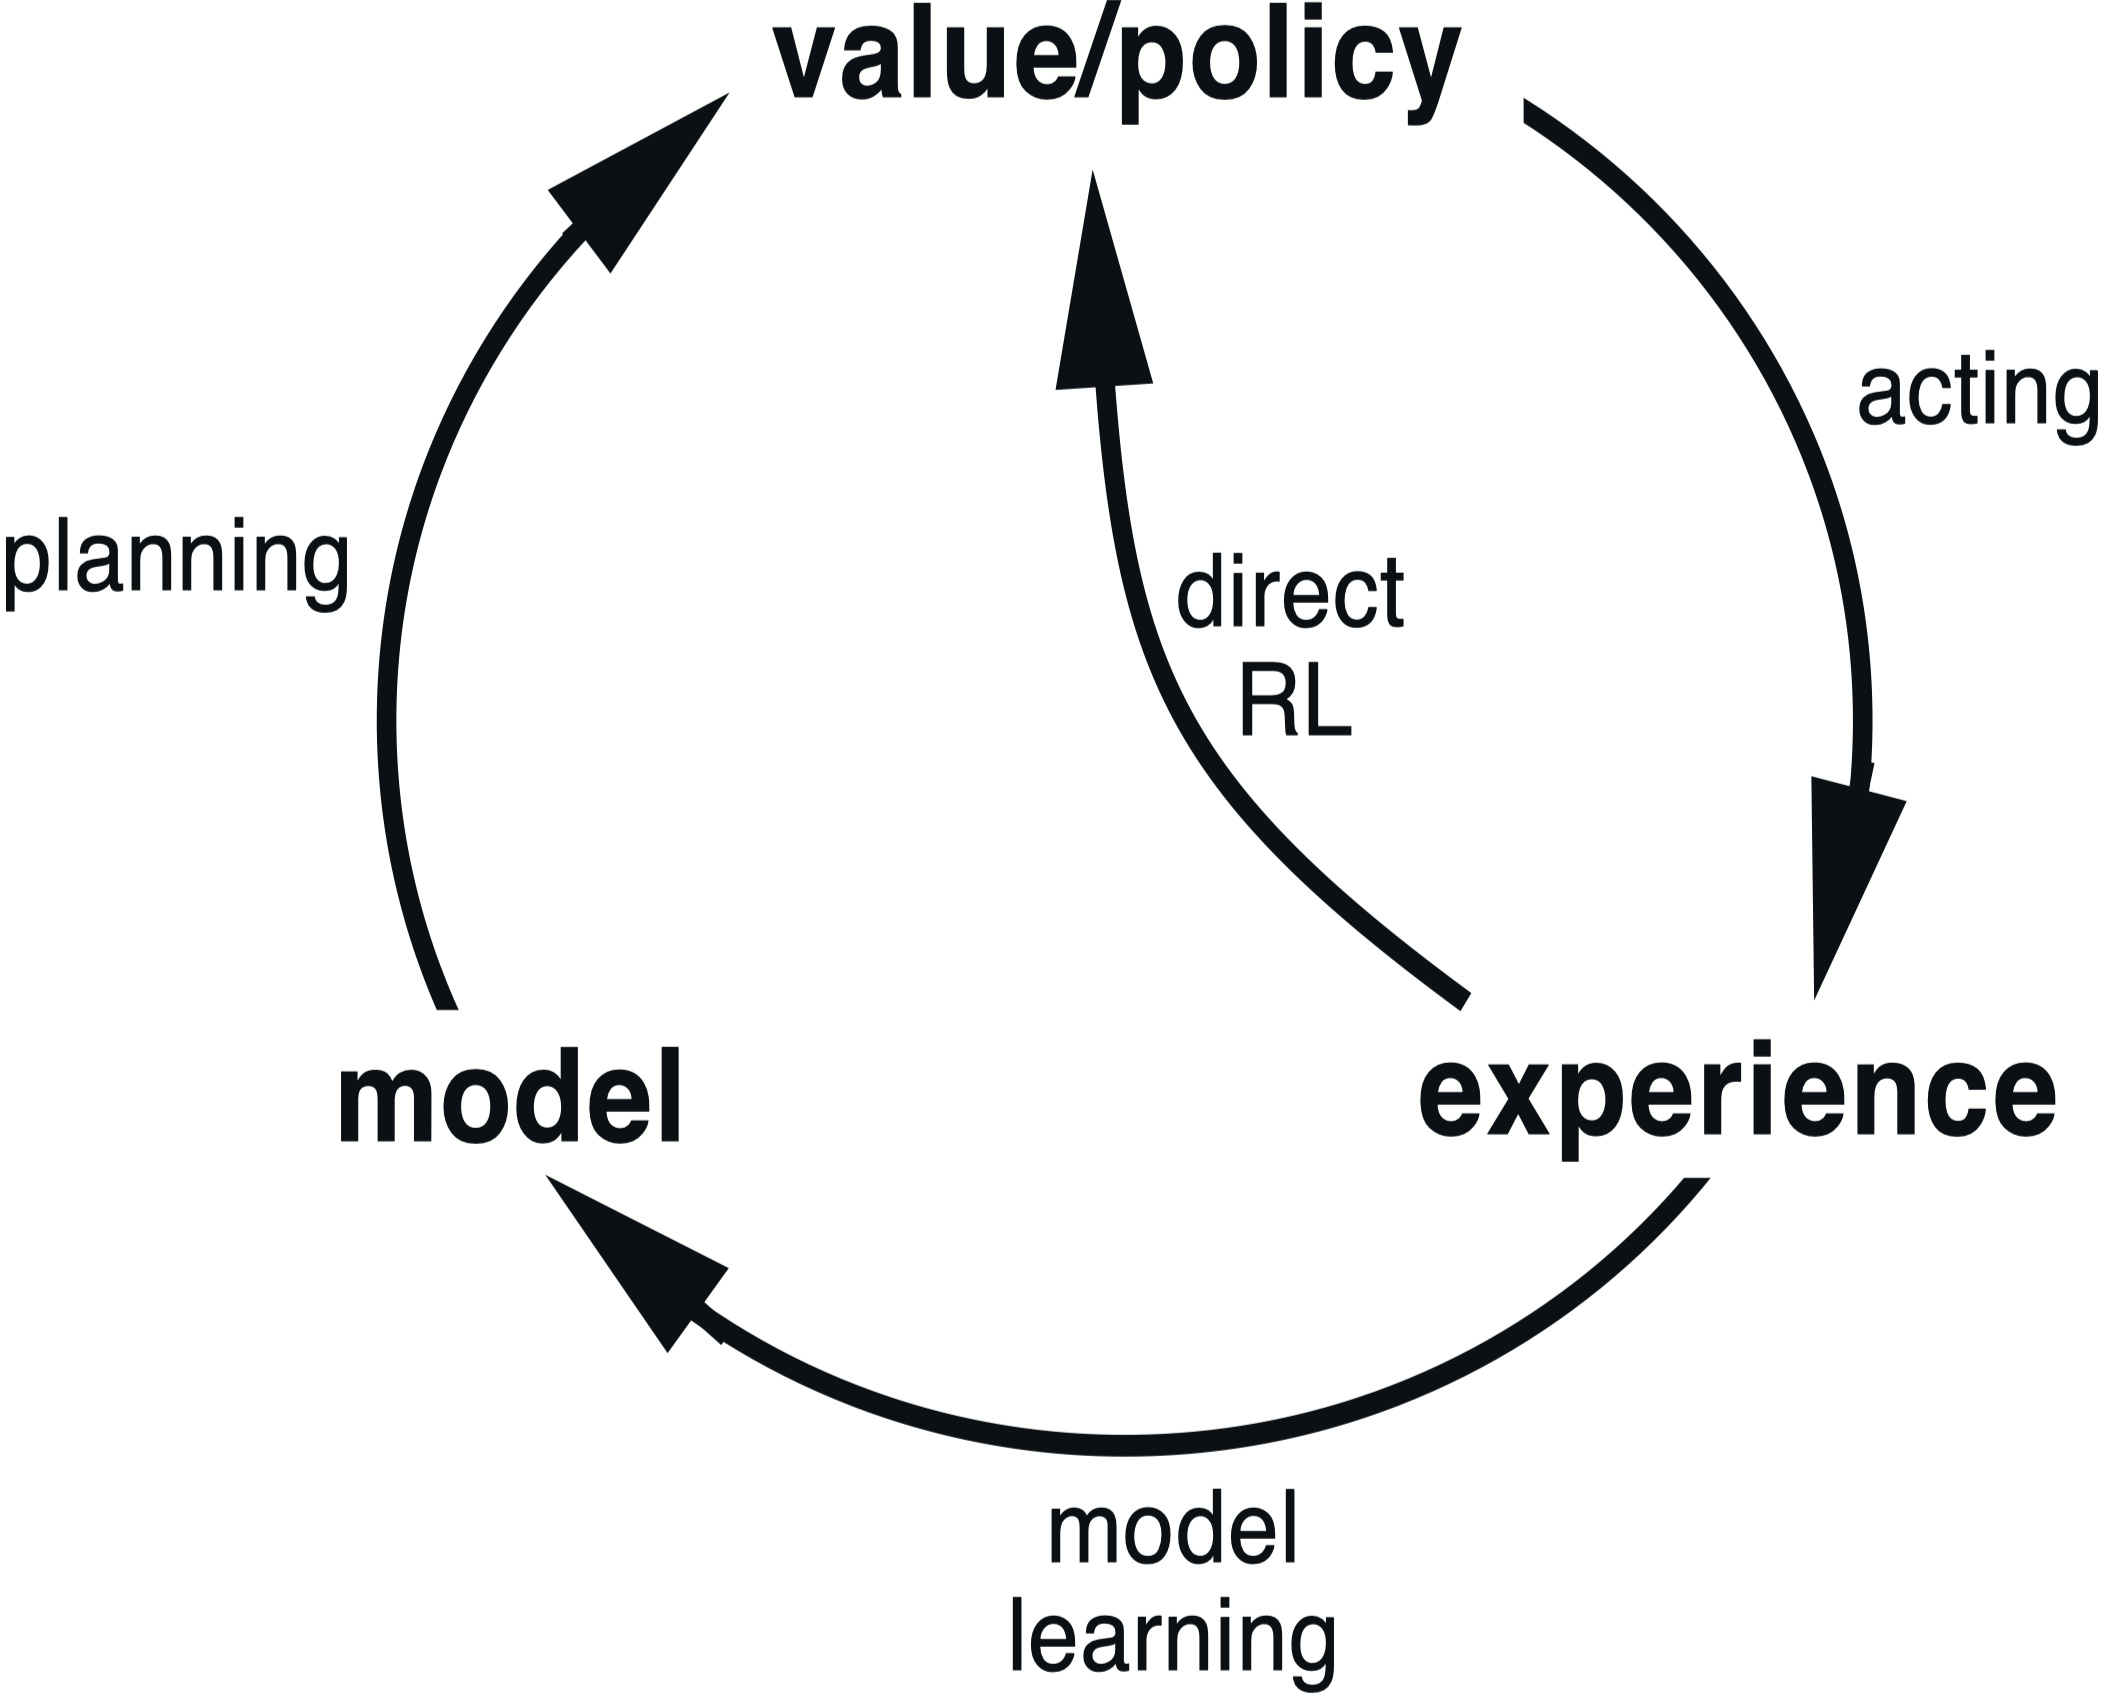
\includegraphics[width=0.66\textwidth]{figures/Dyna.png}
\caption{基于模型的强化学习基本框架。}
\label{fig:dyna-structure}
\end{figure}

\subsection{模型学习的优化}

在学得模型之后,最朴素的用法是,将真实环境数据和模型生成数据 混合,然后执行无模型强化学习方法,这一过程可视作一种数据增广的优化方法。更进阶的模型用法是,使用模型进行上下文信息的辅助计算,从而更高效地加速强化学习算法的收敛速度。

虽然基于模型的强化学习算法有较好的样本效率,但由于模型误差,存在一定的局限性,使用这样有偏差的环境模型去预测,进而会带来更大的误差 \cite{zambaldi2018deep}。

在PILCO方法中 \cite{deisenroth2011pilco},通过学习环境的概率模型,从而实现对复杂环境的不确定性捕捉。具体地,PILCO方法使用了高斯过程回归模型来对环境建模 \cite{quinonero2005unifying},得到环境的概率模型$\mathcal{N}\left(\mu(s_t,a_t), \sigma(s_t,a_t)\right)$,基于这一概率模型,得到期望收益
\begin{equation}
    J^\pi=\mathbb{E}_{s_{t+1}}\left[V\left(s_{t+1}\right)\right]=\int V\left(s_{t+1}\right) \mathcal{N}\left(s_{t+1} \mid \mu_t, \sigma_t\right) \mathrm{d} s_{t+1}
\end{equation}
进而基于梯度$\dfrac{\mathrm{d}J}{\mathrm{d}\theta}$进行策略优化,得到最优参数,使得$\theta^* = {\arg\min}_\theta J^{\pi_\theta}$,最终训练得到最优策略$\pi^*=\pi_{\theta^*}$ 。\cite{peters2006policy}

不确定性环境模型将模型的误差以概率分布的形式展现出来,便能在模型的状态预测环节多次采样得到服从概率分布的预测状态,相比于传统的确定性预测模型,能够让强化学习策略更新环节接收到更多样化的样本输入,从而一定程度上抵消模型偏差带来的影响。但由于高斯过程回归并不适合对复杂的高维度环境进行建模,在后续的PETS方法中,提出使用贝叶斯神经网络(BNN)来对复杂环境进行不确定性建模 \cite{Blundell2015WeightNetworks},从而解决了这一问题。如图\ref{fig:BNN}所示,贝叶斯神经网络的权重不再是固定的权值,而是一个概率分布,神经元间的权值将从这些概率分布中采样得到。

\begin{figure}[tbh]
\centering
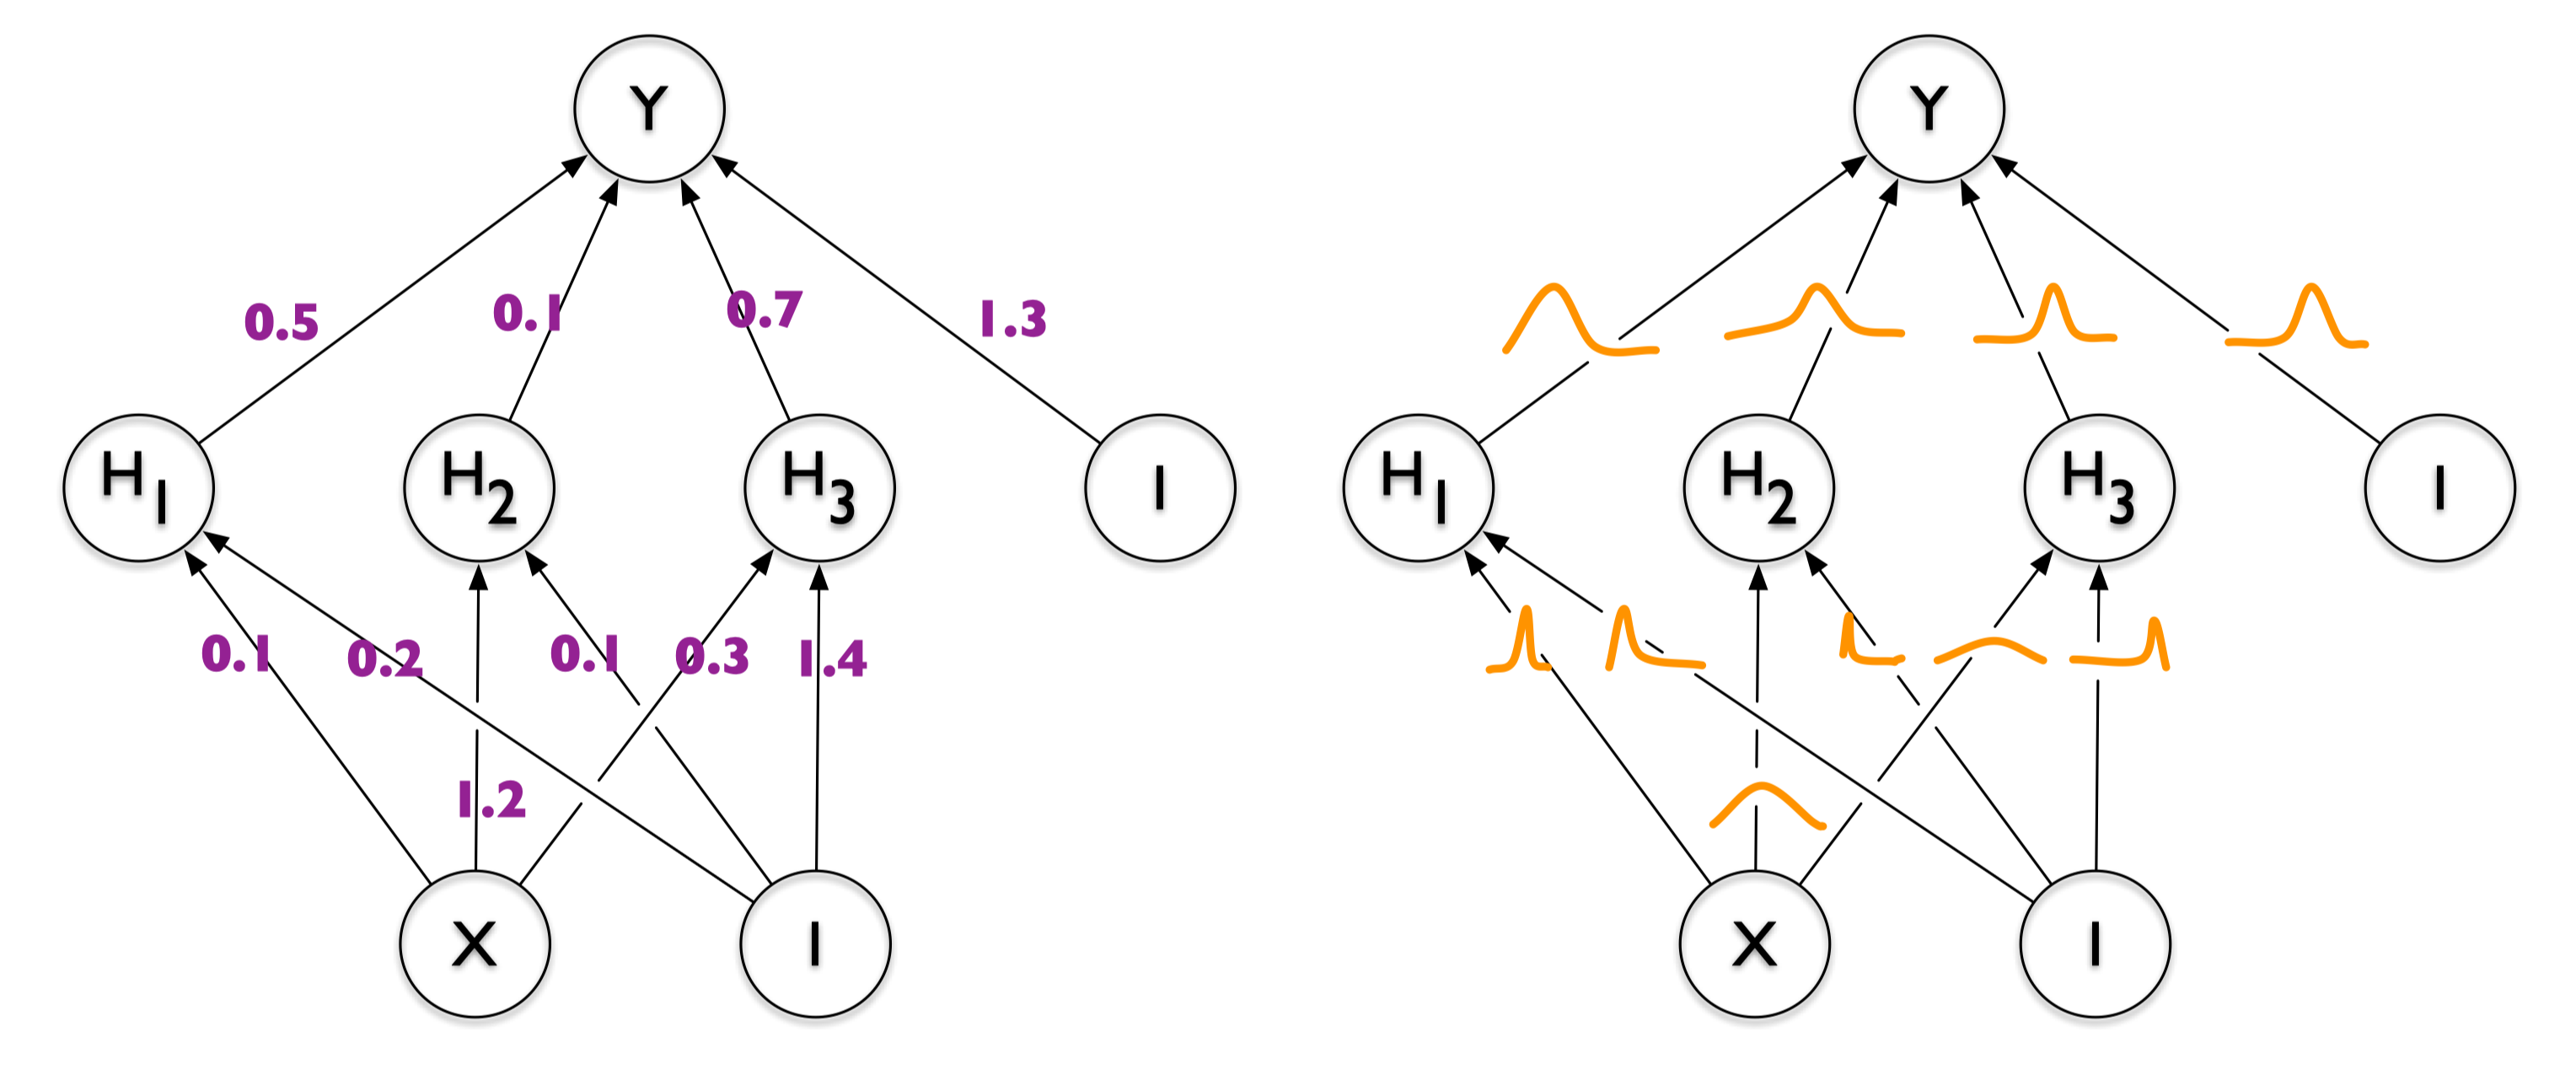
\includegraphics[width=0.9\textwidth]{figures/BNN.png}
\caption{贝叶斯神经网络与普通神经网络的区别。}
\label{fig:BNN}
\end{figure}

\subsection{模型规划的优化}

基于模型的强化学习另一大核心环节便是模型规划 \cite{walsh2010integrating},即使构建出一个准确的环境模型,如果不能合理地利用模型辅助强化学习,对真实样本的利用效率也依然无法得到提升。

在MVE方法中 \cite{feinberg2018model},基于已构建的模型往后展开了$H$步的模拟。由于模型在当前时刻的未来较近步数有着较好的精准度,因此当$H$控制在一个合理范围下时,这$H$步的模拟累积误差相对传统的值函数估计要小很多,将这$H$步模拟替换掉值函数估计,便得到
\begin{equation}
    \hat{V}_{H}\left(s_{0}\right)=\sum_{t=0}^{H-1} \gamma^{t} \hat{r}_{t}+\gamma^{H} \hat{V}\left(\hat{s}_{H}\right)
\end{equation}
MVE将传统无模型强化学习中的值函数学习方法引入模型规划来辅助学习,采用了固定深度的模拟与对剩余部分的估计的结合,实现了模型规划的优化。

在Re-Plan方法中 \cite{williams2017information},每次规划决策得到行动指令,并且基于该指令实际执行行动后,发现真实情况下的转移状态与之前模型规划得到的推理状态之间存在误差,该方法将真实状态进行储存,用作模型预测的修正,从而在下一次规划时,确保模型所预测的有误差状态能被存储记录修正,该方法可以有效地解决模型预测偏差的问题。

而在MBPO方法中 \cite{janner2019trust},证明了当规划长度控制在一个可控长度$k$以内,即

\begin{equation}
k^{*}=\underset{k}{\operatorname{argmin}}\left[\frac{\gamma^{k+1} \epsilon_{\pi}}{(1-\gamma)^{2}}+\frac{\gamma^{k} \epsilon_{\pi}}{(1-\gamma)}+\frac{k}{1-\gamma}\left(\epsilon_{m^{\prime}}\right)\right]>0
\end{equation}

此时,模型的误差始终可以保障在一个误差界限以内,从而在可控的预测误差下,能够最大程度地进行充分的模型规划预测。


\section{本文的主要研究内容}

\section{本文的组织结构}
% !TeX root = ../main.tex

\chapter{预备知识与研究现状}\label{chap:background}

本章主要介绍强化学习的基本概念,

\section{强化学习的基本概念}

强化学习算法的核心框架由智能体和环境构成,其中智能体指决策策略及其可观测的信息,环境则是全部信息空间中智能体以外的所有信息。在强化学习中,环境和智能体都会随时间改变而变化,我们将指定时间下的环境信息集合定义为状态,而状态组成的集合定义为为状态空间 $\mathcal S$ ,而在具体时刻 $t$ 的状态记作 $S_t\in \mathcal S$ 。智能体在给定状态下能执行的决策行为定义为动作,所有可执行的动作定义为动作空间$\mathcal{A}$,一般将给定状态 $S$ 和具体时刻 $t$下的动作记为 $A_t\in\mathcal{A}(s)$ 。

智能体执行 $A_t$ 后,环境信息集合会随之影响而发生改变,由当前状态 $S_t$ 转变为未来状态 $S_{t+1}$ 。在该转变过程中,环境还有一个反馈能力,可以根据动作$A_t$在自身中的表现反馈一个用于评价动作好坏程度的奖励指标 $R_{t}\in\mathcal{R}$ 。定义策略为映射关系:$\pi:\mathcal{S}\times\mathcal{A}\to \mathcal{P}$ ,其中$\mathcal P$表示整体概率空间。策略函数 $\pi(a|s)$ 表示智能体在面对状态 $s$ 时决策采取动作 $a$ 的概率。智能体根据反馈的奖励指标 $R_{t}$ ,可以调整自身策略中对应动作的概率系数,将高奖励反馈的动作赋予更大的执行概率,将低奖励反馈的动作赋予更低的执行概率,通过调整决策策略以使未来的决策动作能收到更好的奖励反馈。这样的策略调整过程称为策略学习或策略优化。

在强化学习中,为了能够计算长期的收益,需要定义完整轨迹上的总收益,一般称这样的总收益为轨迹返回值,可如下所示定义 $t$ 时刻到结束时刻$T$的轨迹返回值 $G_t$ :
\begin{equation}
G_t = R_{t+1}+R_{t+2}+R_{t+3}+\cdots+R_T
\end{equation}
对于无限长轨迹的强化学习问题问题,上述的返回值定义会趋于$\infty$,无法比较动作之间的差异,此时需要重新定义 $G_t$:
\begin{equation}
G_t = R_{t+1}+\gamma R_{t+2}+\gamma^2 R_{t+3}+\cdots = \sum_{k=0}^{\infty}\gamma^kR_{t+k+1}
\end{equation}
其中 $\gamma(0\leq \gamma < 1)$ 为削减系数,通过不断累积削减系数,返回值将表现为更加关注近期时刻的奖励反馈。

\subsection{Markov性质与Markov决策过程}

在强化学习中,我们假定环境满足Markov性质,并将智能体与满足Markov性质的环境进行交互决策的过程称为Markov决策过程(Markov Decision Process,MDP)\cite{white1963dynamic,ross1996stochastic}。在MDP中,每一时刻的状态仅与前一时刻状态相关,与其他任意时刻的状态均无关。Markov性质的定义如下
\begin{definition}
设完整历史信息的联合概率分布为
\begin{equation}
    \mathrm{Pr}\{S_{t+1}=s',R_{t+1}=r|S_0,A_0,R_1,\ldots,R_t,S_t,A_t\}
\end{equation}
设状态转移概率分布为
\begin{equation}
    p(s',r|,s,a) = \mathrm{Pr}\{S_{t+1}=s',R_{t+1}=r|S_t=s,A_t=a\}
\end{equation}
当一个决策过程满足条件$p(s',r|s,a) = \mathrm{Pr}\{S_{t+1}=s',R_{t+1}=r|S_0,A_0,R_1,\ldots,S_t,A_t\}$ ,则称决策过程具有Markov 性质。
\end{definition}

满足Markov性质的决策过程,称为Markov决策过程\cite{sutton2018reinforcement,white1963dynamic}。在满Markov 决策过程中,智能体进行决策时仅需考虑当前时刻的状态信息集合。
此时可定义状态价值函数和动作价值函数:
\begin{equation}
    v_{\pi}(s)=\mathbb{E}_{\pi}\left[G_t|S_t=s\right]=\mathbb{E}_{\pi}\left[\sum_{k=0}^{\infty}\gamma^kR_{t+k+1}\mid S_t=s\right], \forall s \in \mathcal{S}
\end{equation}
\begin{equation}
    q_{\pi}(s,a) =\mathbb{E}_{\pi}\left[G_t|S_t=s,A_t=a\right]=\mathbb{E}_{\pi}\left[\sum_{k=0}^{\infty}\gamma^kR_{t+k+1}\mid S_t=s,A_t=a\right]
\end{equation}
状态价值函数$v_\pi(s)$ 表示智能体以状态$s$为初始状态,通过策略函数 $\pi$ 与环境交互生成决策动作并执行,最终所能得到的轨迹回报值期望;行动价值函数 $q_\pi(s,a)$ 表示只能体以状态 $s$ 为初始状态,在确定执行动作 $a$后 ,通过策略函数 $\pi$ 与环境交互生成决策动作并执行,最终所能得到的轨迹回报值期望。

\subsection{动态规划求解最优策略}

强化学习算法的目标是求解Markov决策过程的最优策略,最优策略和其对应的价值函数定义如下
\begin{definition}
    在概率空间 $\mathcal{P}$ 中存在且至少存在一个策略优于其他所有策略,称满足这一条件的策略为最优策略,记作$\pi^*$,其对应的最优状态价值函数记为 $v_*(s)$,对应的最优动作价值函数记为 $q_*(s,a)$。
\end{definition}

而在有限Markov决策过程中,对于任意前后状态$s$和$s^\prime$,均存在Bellman 最优方程关系\cite{white1963dynamic}:
\begin{equation}\label{eq:v_star}
    v_*(s)=\max_{a}\sum_{s',r}p(s',r \mid s,a)[r+\gamma v_*(s')]
\end{equation}
\begin{equation}\label{eq:q_star}
q_*(s,a) = \sum_{s',r}p(s',r \mid s,a)\left[r+\gamma \max_{a'}q_*(s',a') \right]
\end{equation}

通过求解Bellman最优方差得到解 $v_*,q_*$ ,可进一步推导最优策略的形式,此时可将最优策略定义如下:
\begin{definition}
    记动作价值函数值能达到 $q_*$的动作为 $a_*$,如果一个策略$\pi$仅将非零概率赋予所有满足上述性质的$a_*$,称$pi$为最优策略。
\end{definition}

% 对于状态价值函数的更新公式

% \begin{equation}
% \begin{aligned}
% v_\pi(s) &\doteq \mathbb{E}_\pi[R_{t+1}+\gamma R_{t+2}+ \gamma^2 R_{t+3}+ \cdots \mid S_t = s] \\ 
% &= \mathbb{E}_\pi[R_{t+1}+\gamma v_\pi(S_{t+1}) \mid S_t=s]\\ 
% &=\sum_a\pi(a\mid s)\sum_{s',r}p(s',r\mid s,a)[r+\gamma v_\pi(s')]
% \end{aligned}
% \end{equation}

% 在已知 $p(s',r|s,a)$ 的条件下,那么上 式可视为一个可求解的线性方程组,但考虑到求解速度受限于状态空间$|\mathcal{S}|$的大小,在高维状态空间的复杂场景下难以求解,而使用动态规划的思想便能有效地通过迭代更新来逐步求解出状态值函数,即通过迭代求解法,找到序列 $\{v_k\}$ 使得 $\lim\limits_{k\to\infty}v_k=v_\pi$。

% 将状态值函数 $v_\pi$ 的Bellman方程重写为更新规则式:

% \begin{equation}
% \begin{aligned}v_{k+1}(s) &\doteq \mathbb{E}_\pi[R_{t+1}+\gamma v_k(S_{t+1}) \mid S_t=s] \\ &= \sum_a\pi(a\mid s)\sum_{s',r}p(s',r \mid s,a)[r+\gamma v_k(s')]\end{aligned}
% \end{equation}

% 将方程未知元的系数记为 $c_{ij}$,常数项记为 $b_i$,方程组组可展开为如下形式

% \begin{equation}
% \begin{aligned}
% v_{k+1}(s_1)=&c_{11}v_k(s_1)+c_{12}v_k(s_2)+\cdots+c_{1n}v_k(s_n)+b_1\\
% v_{k+1}(s_2)= & c_{21}v_k(s_1)+c_{22}v_k(s_2)+\cdots+c_{2n}v_k(s_n)+b_2\\
% &\vdots\\
% v_{k+1}(s_n)= & c_{n1}v_k(s_1)+c_{n2}v_k(s_2)+\cdots+c_{nn}v_k(s_n)+b_n\\
% \end{aligned}
% \end{equation}

% 记

% \begin{equation}
% \boldsymbol{C} =
% \begin{bmatrix}
% c_{11} & c_{12} & \cdots & c_{1n}  \\
% c_{21} & c_{22} & \cdots & c_{2n}  \\
% \vdots & \vdots & \ddots & \vdots  \\
% c_{n1} & c_{n2} & \cdots & c_{nn}
% \end{bmatrix}
% \end{equation}

% \begin{equation}
% \boldsymbol{b} =
%     \begin{bmatrix}
%     b_{1} & b_{2} & \vdots & b_{n} 
%     \end{bmatrix}^{\mathrm{T}}
% \end{equation}

% 在矩阵形式下可将Bellman方程的迭代更新规则表示为如下形式:

% \begin{equation}\label{eq:bellman-update}
%     \boldsymbol{v}_{k+1} =\boldsymbol{Cv}_k+\boldsymbol{b}
% \end{equation}

% 由于

% \begin{equation}
% \begin{aligned}
%         c_{ij} &=\sum_a\pi(a\mid s_i)\sum_{r}p(s_j,r \mid s_i,a)\gamma\\
%         &\leq \sum_a\pi(a\mid s_i)\sum_{s_j,r}p(s_j,r \mid s_i,a)\gamma=\gamma
%     \end{aligned}
% \end{equation}

% \begin{equation}
% b_{i} =\sum_a\pi(a\mid s_i)\sum_{r}p(r\mid s_i,a)r
% \end{equation}

% 根据定义 $0\leq\gamma<1$,可以计算上述方程的系数矩阵极限为零矩阵:

% \begin{equation}
% \lim_{k\rightarrow \infty} \boldsymbol{C}^k \leq \lim_{k\rightarrow \infty}\begin{bmatrix}
%     \gamma & \gamma & \cdots & \gamma\\
%     \gamma & \gamma & \cdots & \gamma\\
%     \vdots & \vdots & \ddots & \vdots\\
%     \gamma & \gamma & \cdots & \gamma
%     \end{bmatrix}^k = \boldsymbol{O}
% \end{equation}

% 即 $\boldsymbol{C}^k\rightarrow\boldsymbol{O}$,根据Jacobi 迭代法的收敛定理,可以证明方程(\ref{eq:bellman-update})一定可以通过Jacobi迭代法快速求解得到收敛解。

基于以上定义可知,理论上求解 Bellman 最优方程即意味着求解得到最优策略,但由于Bellman方程难以直接求解仅存在理论可解性,实际中需要使用动态规划的思想来迭代求解Bellman关系式获取$v_*,q_*$的近似解\cite{sutton2018reinforcement}。在通过动态规划求解得到的价值函数之后,则需考虑如何使用这一价值函数用于优化决策策略$\pi$。具体的做法是将上述的值估计求解算法与策略优化算法相结合,并进行循环优化。策略优化算法的核心思路是按照如下公式选取最优动作$a$替换原有策略中的部分决策:

\begin{equation}
    \begin{aligned}\pi'(s) &= \mathop{\arg\max}\limits_a q_\pi(s, a)\\&=\mathop{\arg\max}\limits_a \mathbb{E}[R_{t+1}+\gamma v_\pi(S_{t+1})\mid S_t=s,A_t=a] \\&= \mathop{\arg\max}\limits_a \sum_{s',r} p(s', r | s, a) (r + \gamma v_\pi(s'))\end{aligned}
\end{equation}

将策略价值函数估计(Policy Evaluation)简记为E步骤,由符号“$\xrightarrow{E}$”表示;策略优化(Policy Improvement)简记为I步骤,由符号“$\xrightarrow{I}$”表示。则上述的循环优化过程可以表示为如下所示的流程
\begin{equation}
\pi_0 \xrightarrow{E} v_{\pi_0} \xrightarrow{I}\pi_1 \xrightarrow{E} v_{\pi_1} \xrightarrow{I} \pi_2 \xrightarrow{E} \cdots \xrightarrow{I} \pi_* \xrightarrow{E} v_*
\end{equation}

在有限Markov决策过程中,状态空间$\mathcal{S}$和行为动作空间$\mathcal{A}$都是有限的,显然可见策略空间也是有限的。而考虑到在策略价值函数估计和策略优化的循环过程中价值函数存在上界且单调递增,由单调收敛定理可知,存在一个步数$N$,当循环次数大于$N$后,所得策略能够近似逼近理想最优策略。

\section{策略梯度优化}

尽管动态规划算法能够理论上学习得到足够接近最优的策略,但直接求解的方法并没有充分发挥深度机器学习的优势。通过将策略函数进行参数化的做法,可以有效地结合机器学习中的梯度上升/下降算法,更为高效地进行策略学习。首先定义参数化的策略函数:
\begin{equation}
\pi ( a | s , \boldsymbol { \theta } ) = \operatorname { Pr } \left\{ A _ { t } = a | S _ { t } = s , \boldsymbol { \theta } _ { t } = \boldsymbol { \theta } \right\}
\end{equation}
使用参数化决策策略所产生的价值函数,可定义参数化的性能目标函数:
\begin{equation}
    J(\boldsymbol{\theta}) \doteq v_{\pi_{\boldsymbol{\theta}}}\left(s_{0}\right)
\end{equation}
其中 $v_{\pi_{\boldsymbol{\theta}}}\left(s_{0}\right)$ 是 $\pi_\theta$ 初始状态为$s_0$条件下的真实价值函数 ,其中策略由 $\boldsymbol{\theta}$ 决定。通过对价值函数 $J ( \boldsymbol { \theta } )$ 的梯度进行梯度更新优化,可以实现性能的最优化,即
\begin{equation}
\boldsymbol { \theta } _ { t + 1 } = \boldsymbol { \theta } _ { t } + \alpha \widehat { \nabla J \left( \boldsymbol { \theta } _ { t } \right) }
\end{equation}
其中$\widehat { \nabla J \left( \boldsymbol { \theta } _ { t } \right) } \in \mathbb { R } ^ { d ^ { \prime } }$ 是梯度的估计值,满足$E_\boldsymbol{\theta}\left[\widehat { \nabla J \left( \boldsymbol { \theta } \right) }\right]=\nabla V(\boldsymbol{\theta})$,即其期望值为真实的梯度。基于以上的定义,可以给出如下定理:
\begin{theorem}
给定状态访问概率分布$\mu(s)$、行动价值函数$q_\pi(s,a)$,性能目标函数的梯度$\nabla J(\boldsymbol{\theta})$与策略函数的梯度$\pi(a | s, \boldsymbol{\theta})$存在如下所示的正比关系:
\begin{equation}
    \nabla J(\boldsymbol{\theta}) \propto \sum_{s} \mu(s) \sum_{a} q_{\pi}(s, a) \nabla \pi(a | s, \boldsymbol{\theta})
\end{equation}
\end{theorem}

\begin{equation}
    \nabla J(\boldsymbol{\theta}) \propto \sum_{s} \mu(s) \sum_{a} q_{\pi}(s, a) \nabla \pi(a | s, \boldsymbol{\theta})
\end{equation}
这一定理的意义在于,当我们直接优化目标函数的梯度$\nabla J(\boldsymbol{\theta})$时,等价于在对策略函数$\pi$进行梯度优化,即目标函数$J(\boldsymbol{\theta})$的最优化参数$\boldsymbol{\theta_*}$也是策略函数$\pi(a|s,\theta)$的最优化参数。在该定理的保证下,我们可以直接对$J(\boldsymbol{\theta})$进行简单的梯度优化即可求得最优策略。

\section{经验样本回放}

在Q-Learning、SARSA\cite{watkins1992q,sutton2018reinforcement}等传统的强化学习算法中,环境交互样本往往只被使用一次后便被立即放弃,不再重复使用。由于其中的一些样本含有较高的学习价值,训练一次后即被丢弃的做法非常不利于强化学习算法的样本效率,基于这一考虑,经验回放的方法得以提出\cite{lin1992self},它将重要的经验存储在样本池中加以多次重复利用,使得智能体能够学习过去的经验。不过经验回放也存在一些局限性,如果智能体所处环境随时间会发生变化,过去的经验将完全无助于实时的策略学习。DQN算法\cite{mnih2013playing}将经验回放机制与强化学习算法相结合,对经验回放的样本进行了随机化处理,保证了样本的独立同分布特性,从而解决了经验回放的局限性,在保证算法稳定性的同时做到了样本效率的提升。

尽管DQN算法中所使用的经验回放机制借由随机性改进做到了算法样本效率的优化,但是仍然较为局限。后续的工作提出,在样本池中按优先级进行经验回放的做法将会更加有效,这样的算法称为优先经验回放算法(Prioritized Experience Replay, PER)\cite{schaul2015prioritized}。PER算法能够给更重要的样本赋予更高的优先级,确保更有价值的经验得到更多的回放,从而起到了提升样本效率的效果。在PER算法中,最为理想的方法是计算智能体在样本池中的样本上学习的次数,被学习次数越少的样本,越应该被优先提供给智能体进行学习,然而学习次数这个指标实际上不容易取得。更可行的方案是使用时序差分误差来辅助计算样本池中的采样优先级,时序差分误差大的样本,意味着策略在该样本所处状态上的决策效果存在较大改进空间,同样可以被认为是更有高学习价值的经验样本\cite{tesauro1995temporal},因此需要为其分配更高的优先级进行学习。

实验可以证明,PER算法在诸多测试环境下均取得了大幅的优化改进。不过PER算法的一个缺点是因为修改了样本池中的经验分布,基于强化学习的理论分析可知,经验分布的变动将会导致智能体学习有偏差的策略,因此,PER算法还需要重要性采样(Importance Sampling)\cite{tokdar2010importance}和分布修正估计(Distribution Correction Estimation)\cite{lee2021optidice}等技术加以辅助,用以修正其带来的经验分布偏差。然而对于这一问题,现有的方法仍然有种种不足之处,例如重要性采样方法实际中难以准确计算分布偏差,而分布修正估计方法依赖大量的计算资源,代价高昂。

经验回放的样本选取过程是众多研究工作所关注的一大重点,但与此同时,经验回放样本池的设计也是影响经验回放方法效果的一个重要因素。相关工作已经证明,经验回放样本池的容量会对经验回放算法的效果产生显著影响,过大或过小的的样本池均可导致算法的效率大幅下降\cite{zhang2017deeper}。导致这一现象的原因主要是当经验回放样本池填充满后需要丢弃一部分历史经验,传统的做法是直接按存储时间来依次丢弃,一些工作提出,不同的丢弃方式也将影响经验回放算法的效率\cite{pieters2016q}。

经验回放样本池的另一大研究重点是其中的样本分布。考虑到强化学习对探索和利用机制的需求,如果样本池中的样本分布仅能覆盖实际样本分布中的一小部分,则很可能导致初期训练过拟合、策略脱离实际分布、灾难性遗忘等诸多问题。为了解决上述提到的问题,相关工作提出,更高频地使用最新样本即时覆盖旧样本,可以更有效地帮助智能体学习探索经验\cite{de2015importance}。此外,还可以根据样本的时序差分误差、状态空间占比、奖励反馈等多个指标进行优先级覆盖,从而得以从不同角度解决经验回放方法的缺点。

\section{基于模型的强化学习方法}

尽管经验回放方法通过重复利用现有样本的做法使得强化学习算法的样本利用效率得到一定程度的提升,但其提升程度并不明显,基于模型的强化学习算法是另一类可以有效提升样本利用效率的方法,它通过监督学习训练得到环境状态转移模型,以该模型为模拟环境大量且快速地生成模拟样本,能够辅助策略学习,加速策略的收敛。基于模型的强化学习基本框架最早在1991年提出 \cite{Sutton1991DynaReacting},它实际上是一种模块化的思路,可以应用到现有的各种无模型强化学习算法算法中(例如PPO ,TD3,SAC等算法 \cite{schulman2017proximal,haarnoja2018soft}),旨在高效的利用经验数据,提高学习效率以及数据利用效率。如图~\ref{fig:dyna-structure}~所示,基于模型的强化学习算法融合了规化、决策和学习的方法,在传统的无模型强化学习方法基础上,增加了模型学习$\longrightarrow$模型$\longrightarrow$模型规划的过程 \cite{lin1992self},通过经验数据学习得到一个环境的模型,然后使用模型进行模拟规划,生成模拟数据辅助强化学习进行策略优化更新。

\begin{figure}[tbh]
\centering
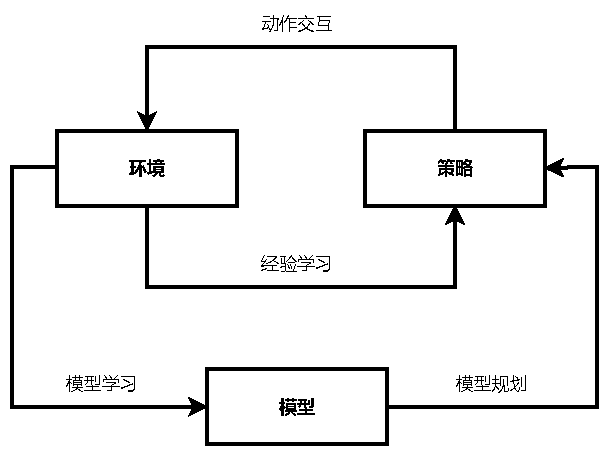
\includegraphics[width=0.8\textwidth]{figures/MBRL-struc.pdf}
\caption{基于模型的强化学习算法基本框架}
\label{fig:dyna-structure}
\end{figure}

在学得模型之后,最朴素的用法是,将真实环境数据和模型生成数据 混合,然后执行无模型强化学习方法,这一过程可视作一种数据增广的优化方法。更进阶的模型用法是,使用模型进行上下文信息的辅助计算,从而更高效地加速强化学习算法的收敛速度。虽然基于模型的强化学习算法有较好的样本效率,但由于模型误差,存在一定的局限性,使用这样有偏差的环境模型去预测,进而会带来更大的误差 \cite{zambaldi2018deep}。

在PILCO方法中 \cite{deisenroth2011pilco},通过学习环境的概率模型,从而实现对复杂环境的不确定性捕捉。具体地,PILCO方法使用了高斯过程回归模型来对环境建模 \cite{quinonero2005unifying},得到环境的概率模型$\mathcal{N}\left(\mu(s_t,a_t), \sigma(s_t,a_t)\right)$,基于这一概率模型,得到期望收益
\begin{equation}
    J^\pi=\mathbb{E}_{s_{t+1}}\left[V\left(s_{t+1}\right)\right]=\int V\left(s_{t+1}\right) \mathcal{N}\left(s_{t+1} \mid \mu_t, \sigma_t\right) \mathrm{d} s_{t+1}
\end{equation}
进而基于梯度$\dfrac{\mathrm{d}J}{\mathrm{d}\theta}$进行策略优化,得到最优参数,使得$\theta^* = {\arg\min}_\theta J^{\pi_\theta}$,最终训练得到最优策略$\pi^*=\pi_{\theta^*}$ 。\cite{peters2006policy}

不确定性环境模型将模型的误差以概率分布的形式展现出来,便能在模型的状态预测环节多次采样得到服从概率分布的预测状态,相比于传统的确定性预测模型,能够让强化学习策略更新环节接收到更多样化的样本输入,从而一定程度上抵消模型偏差带来的影响。但由于高斯过程回归并不适合对复杂的高维度环境进行建模,在后续的PETS方法中,提出使用贝叶斯神经网络(BNN)来对复杂环境进行不确定性建模 \cite{Blundell2015WeightNetworks},从而解决了这一问题。如图~\ref{fig:BNN}~所示,贝叶斯神经网络的权重不再是固定的权值,而是一个概率分布,神经元间的权值将从这些概率分布中采样得到。

\begin{figure}[tbh]
\centering
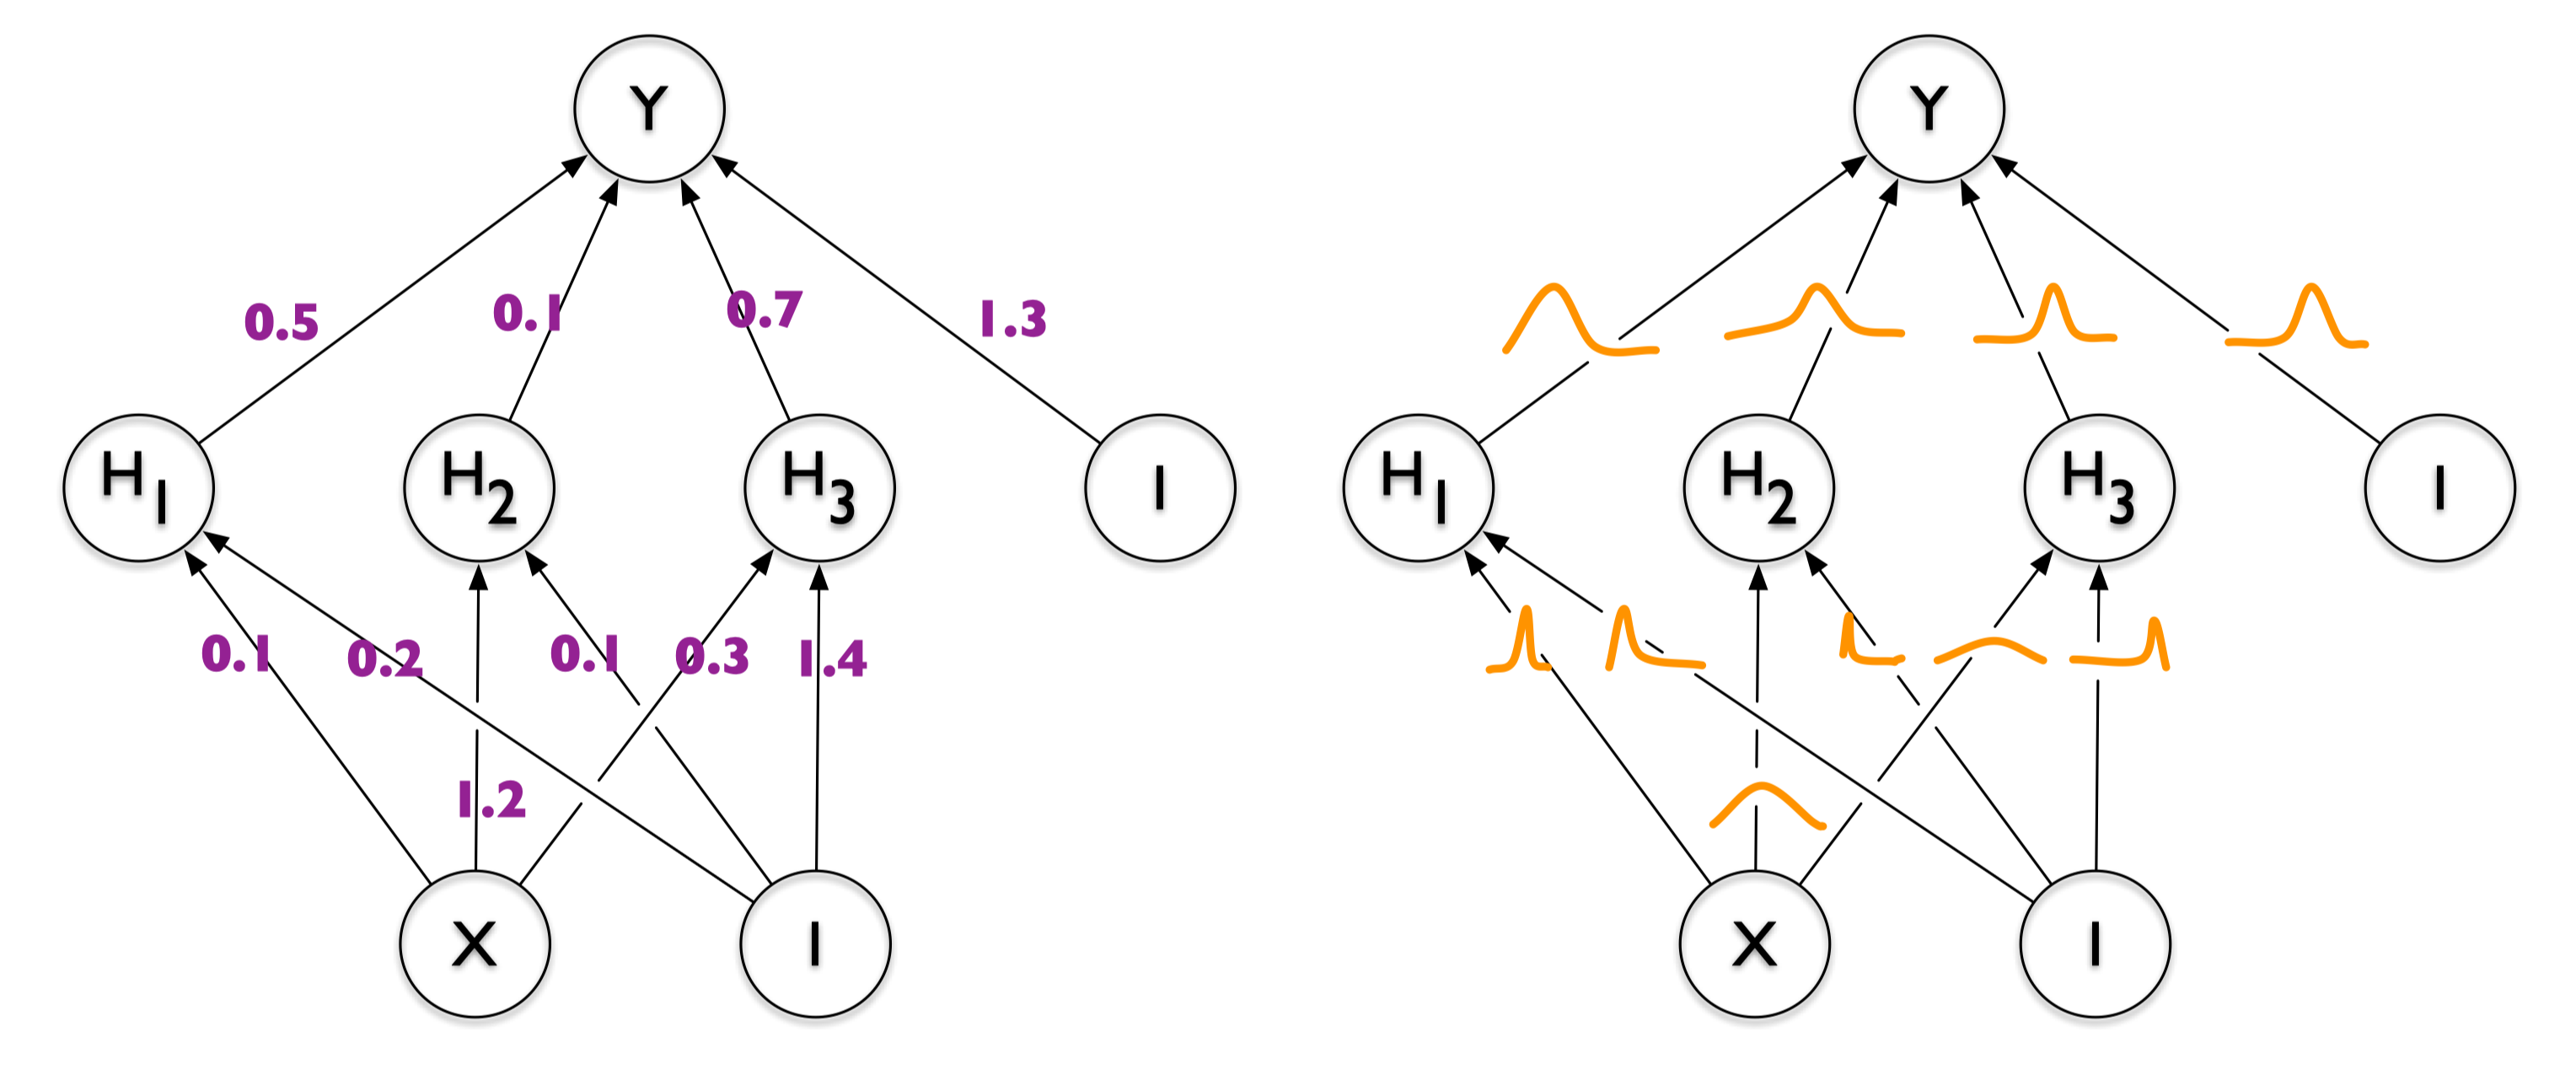
\includegraphics[width=0.9\textwidth]{figures/BNN.png}
\caption{贝叶斯神经网络与普通神经网络的区别}
\label{fig:BNN}
\end{figure}

基于模型的强化学习另一大核心环节便是模型规划 \cite{walsh2010integrating},即使构建出一个准确的环境模型,如果不能合理地利用模型辅助强化学习,对真实样本的利用效率也依然无法得到提升。在MVE方法中 \cite{feinberg2018model},基于已构建的模型往后展开了$H$步的模拟。由于模型在当前时刻的未来较近步数有着较好的精准度,因此当$H$控制在一个合理范围下时,这$H$步的模拟累积误差相对传统的值函数估计要小很多,将这$H$步模拟替换掉值函数估计,便得到
\begin{equation}
    \hat{V}_{H}\left(s_{0}\right)=\sum_{t=0}^{H-1} \gamma^{t} \hat{r}_{t}+\gamma^{H} \hat{V}\left(\hat{s}_{H}\right)
\end{equation}
MVE将传统无模型强化学习中的值函数学习方法引入模型规划来辅助学习,采用了固定深度的模拟与对剩余部分的估计的结合,实现了模型规划的优化。

在Re-Plan方法中 \cite{williams2017information},每次规划决策得到行动指令,并且基于该指令实际执行行动后,发现真实情况下的转移状态与之前模型规划得到的推理状态之间存在误差,该方法将真实状态进行储存,用作模型预测的修正,从而在下一次规划时,确保模型所预测的有误差状态能被存储记录修正,该方法可以有效地解决模型预测偏差的问题。

而在MBPO方法中 \cite{janner2019trust},证明了当规划长度控制在一个可控长度$k$以内,即
\begin{equation}
k^{*}=\underset{k}{\operatorname{argmin}}\left[\frac{\gamma^{k+1} \epsilon_{\pi}}{(1-\gamma)^{2}}+\frac{\gamma^{k} \epsilon_{\pi}}{(1-\gamma)}+\frac{k}{1-\gamma}\left(\epsilon_{m^{\prime}}\right)\right]>0
\end{equation}
此时,模型的误差始终可以保障在一个误差界限以内,从而在可控的预测误差下,能够最大程度地进行充分的模型规划预测。

\section{基于条件风险价值的样本筛选方法}

虽然目前基于模型的强化学习方法已经取得了显著的样本利用效率提升效果,但它们通常只适合于其所训练的环境,当部署到扰动的真实环境时,性能往往会急剧下降。

\begin{figure}
  \centering
  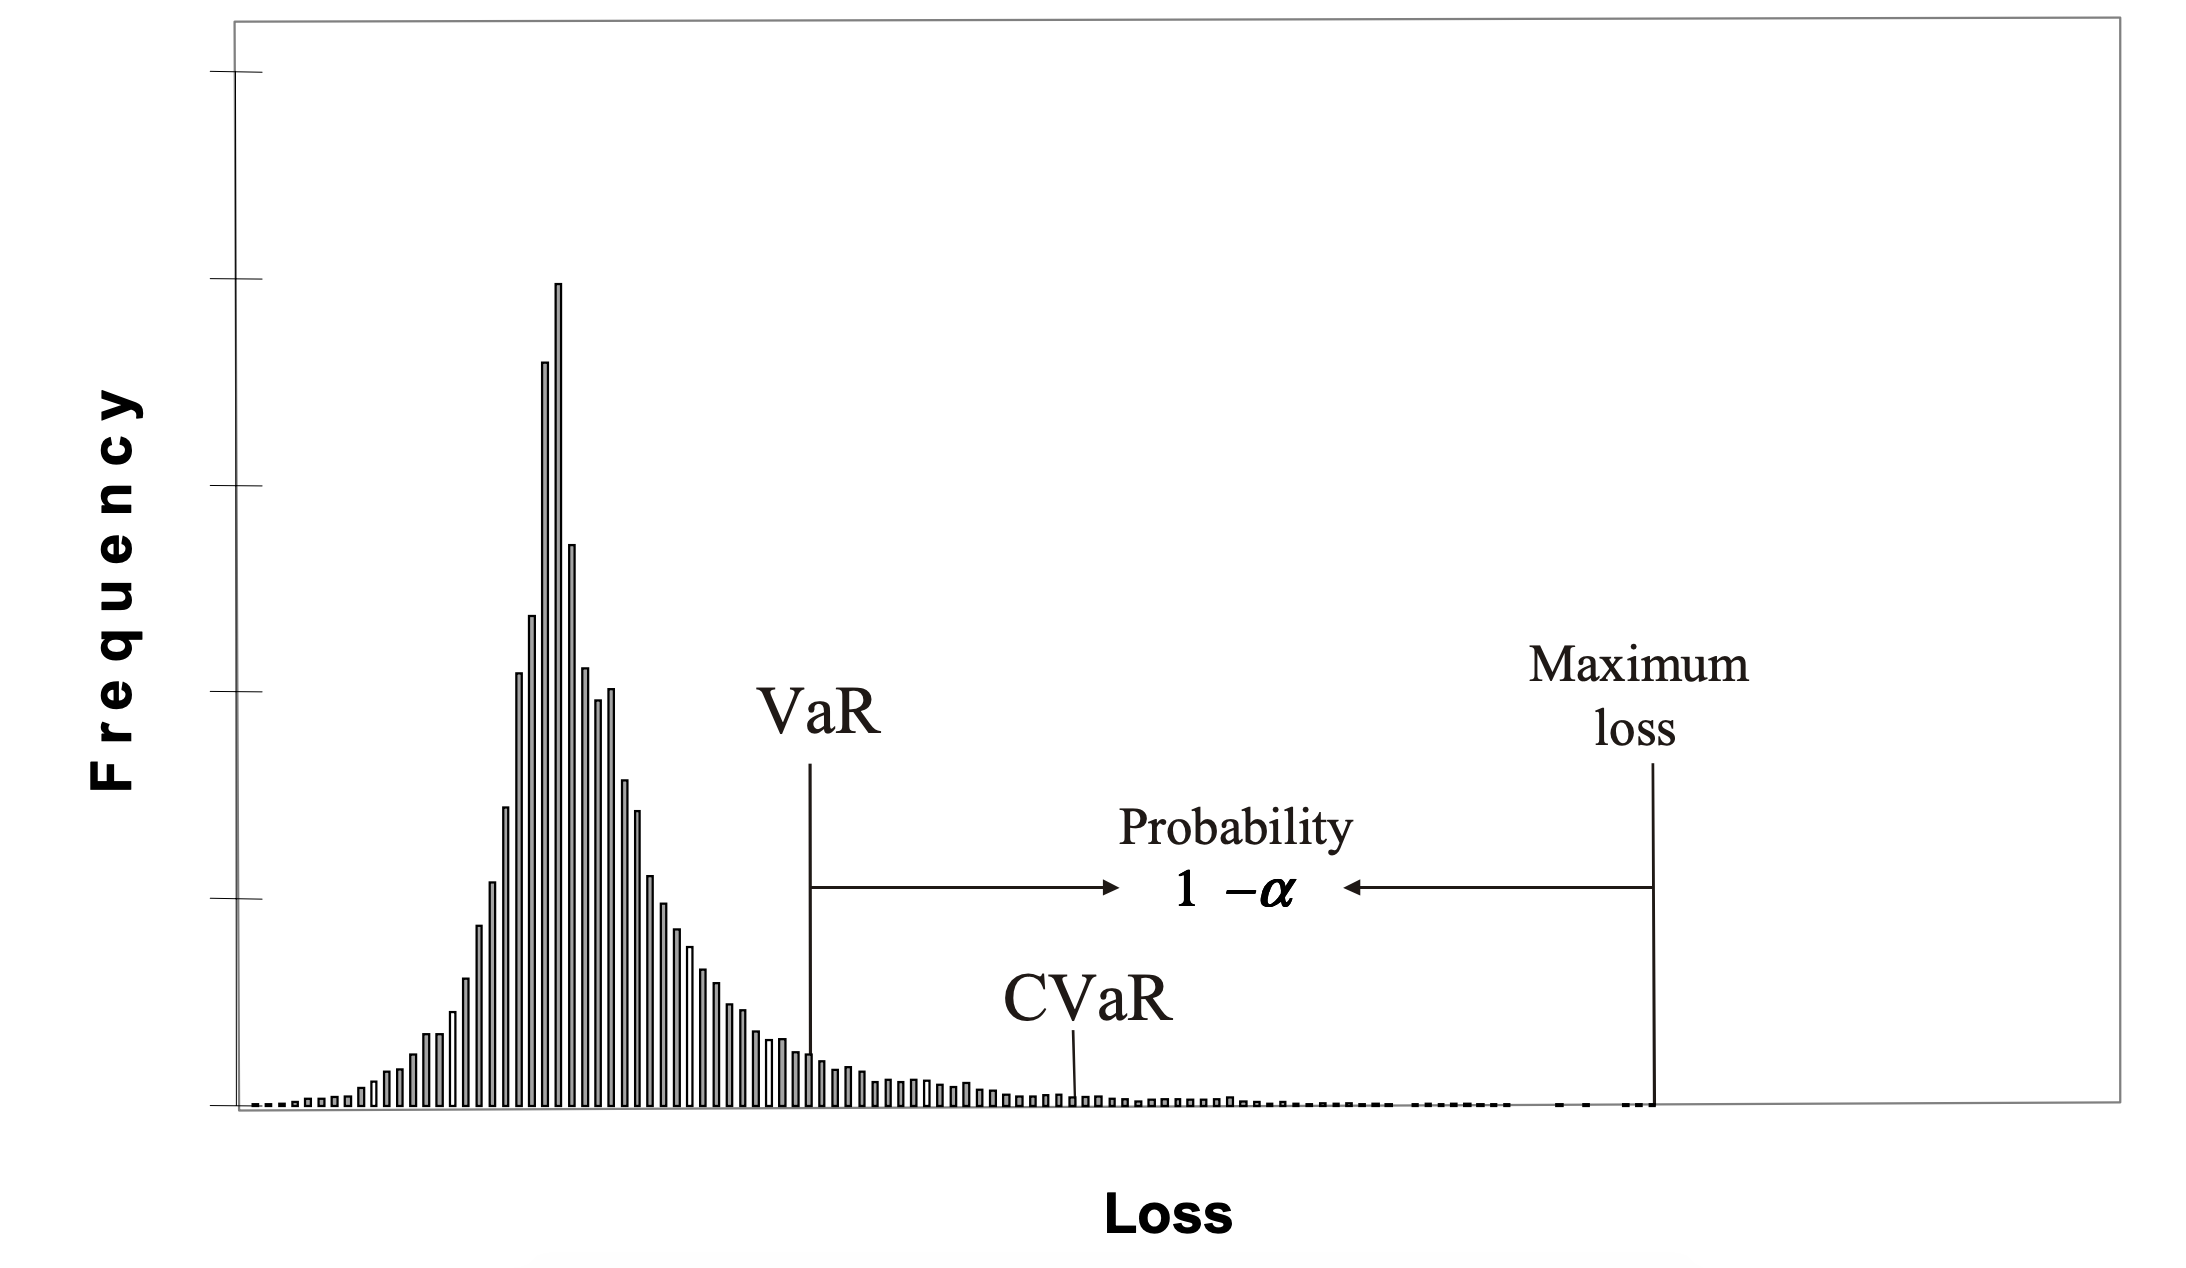
\includegraphics[width=\linewidth]{figures/CVaR.png}
  \caption{CVaR计算示意图}
  \label{fig:cvar}
\end{figure}

条件风险价值(CVaR)是一种用于计算最大风险的指标,如图\ref{fig:cvar}所示,首先需要定义风险价值(VaR)。记$Z$为随机变量,其累积分布函数为$F(z)=\mathrm{Pr}(Z<z)$,给定置信度$p \in (0,1)$,则关于 $Z$ 的$p$-置信度风险价值定义为$\mathrm{VaR}_p(Z)$:
\begin{equation}
    \mathrm{VaR}_p(Z)=F^{-1}(p)\triangleq \inf\{z:F(z)\geq p\}.
\end{equation}
更进一步地,我们可定义条件风险价值(CVaR)。记关于$Z$的置信度$p$条件风险价值为$\mathrm{CVaR}_p(Z)$,其定义为关于随机变量$Z$的$p$百分比末尾分布期望值:
\begin{equation}\label{eq:def-cvar}
    \mathrm{CVaR}_p(Z)\triangleq \mathbb{E}[Z|Z\geq \mathrm{VaR}_p(Z)].
\end{equation}

CVaR的含义可解释为收益风险超过VaR部分的平均期望损失。借由CVaR指标,我们可以通过学习消极样本数据来提高强化学习算法的鲁棒性,得以解决强化学习算法中安全性不足的一大挑战。一些现有工作已经尝试以CVaR的思想,设计了样本筛选机制\cite{rajeswaran2016epopt},通过丢弃部分返回值更低的轨迹样本,适度抑制算法的学习速率,起到引导智能体更加关注低回报轨迹样本的作用,从而确保所学策略在面对异常状态时仍能保持较好的决策效果。实验表明,基于CVaR思想设计的样本筛选方法尽管可以一定程度地提升策略的整体稳定性和鲁棒性,但其也存在降低策略学习速度,减小样本利用效率等不足之处。

\section{本章小结}

本章主要介绍了强化学习的基本概念,从基本的Markov性质及Markov决策过程出发,介绍了以Bellman方程为核心的动态规划求解方法,以及以梯度下降为核心的策略梯度优化方法等预备知识。并根据强化学习中样本效率问题及策略安全性问题的研究现状,介绍了经验样本回放方法,基于模型的强化学习和基于条件风险价值的筛选方法。
% !TeX root = ../main.tex

\chapter{基于双层缓存的优先经验回放算法}\label{chap:dper}

在第~\ref{chap:intro}~章中我们已经介绍,尽管使用随机抽取经验样本进行回放的做法能够对算法样本效率起到一定的优化,但是仍然较为局限。而PER算法在样本池中按优先级进行经验回放的做法则更加有效,能够给更重要的样本赋予更高的优先级,确保更有价值的经验得到更多的回放,从而起到了提升样本效率的效果。在PER算法中,理想的设计方案是计算样本池中的样本被用于学习的次数,次数越少,说明该样本越应被优先提供给智能体进行学习。考虑到该指标在实际运行时难以获取,选择了使用时序差分误差来辅助计算样本池中的采样优先级作为替代方案,这是因为时序差分误差大的样本,意味着策略在该样本所处状态上的决策效果存在较大改进空间,同样可以被认为是更有高学习价值的经验样本,因此需要为其分配更高的优先级进行学习。尽管优先经验回放方法已经在强化学习中取得了很好的效果,但它仍有很多局限性:

\begin{enumerate}
    \item 为避免扫描整个样本回放池的昂贵成本,只有被回放过的经验样本的时序差分误差值会被更新,这将导致一些有较小的初始误差值样本长时间不被回放,进而对整个样本空间覆盖率不高
    \item 时序差分误差对噪声非常敏感,很容易因噪声而增加估计误差,同时较高的时序差分误差带来的频繁回放会因损失多样性而导致算法过拟合
    \item PER只对由访问过的状态组成的回放样本池进行优先级分配。与整个状态空间相比,样本池可能只覆盖其中一个小的子集,实际中并不能实现全局意义上的优先级分配就无法实现,与其设计理念相差甚远。
\end{enumerate}

这些问题在现有的工作中并没有得到太多关注,为此,我们设计了基于双层缓存的优先经验回放算法,可以有效解决上述提到的优先经验回放算法的局限性,学习更多的重要经验,提升强化学习的样本效率效率。

\section{双层经验样本回放池及回放算法设计}

\begin{figure}[ht]
\centering
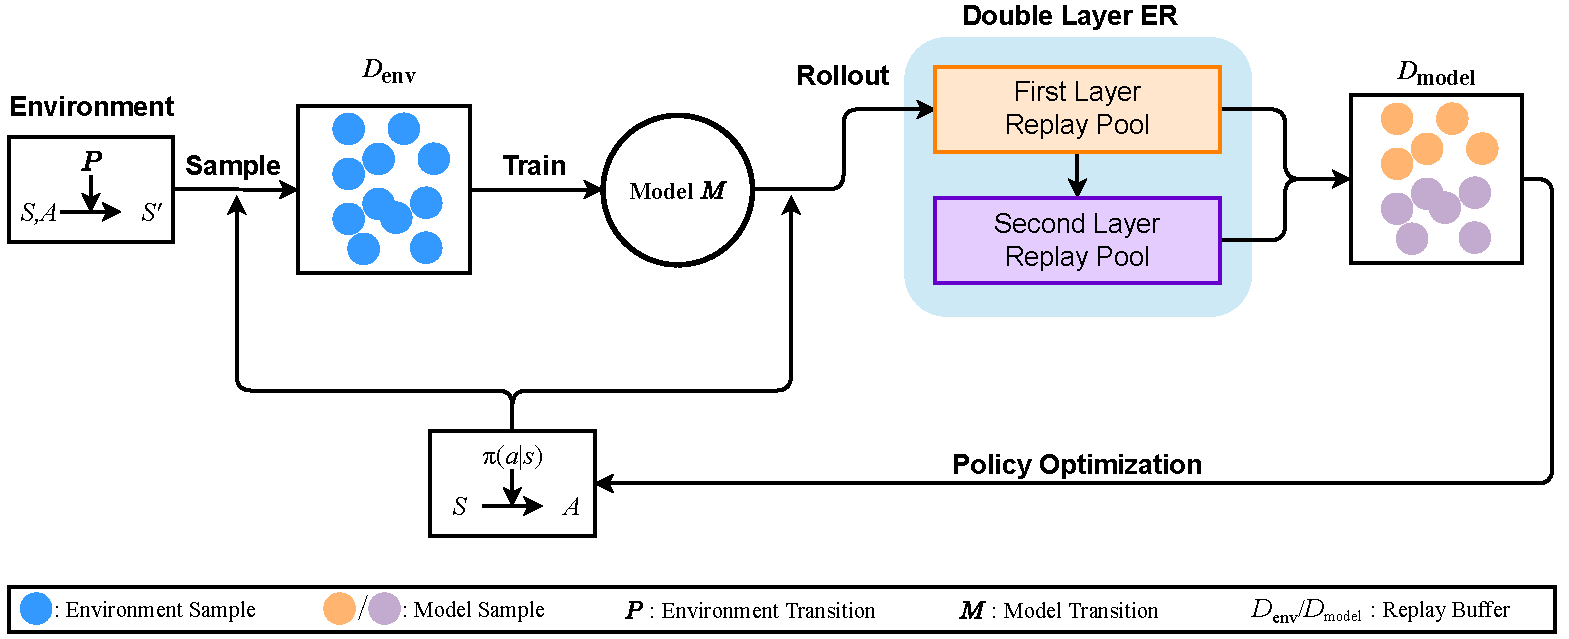
\includegraphics[width=\textwidth]{figures/dber.pdf}
\caption{基于双层缓存的优先经验回放算法示意图}
\label{fig:algo-structure}
\end{figure}

经验回放算法中,回放样本池的设计是影响经验回放方法效果的一个重要因素。Zhang等人在论文\cite{zhang2017deeper}中提出,经验回放样本池的大小会对经验回放算法的效果产生显著影响,过大或过小的的样本池均可导致算法的效率大幅下降。其主要原因经验回放样本池中的历史经验一旦填满,则会开始丢弃旧的样本,这一特性限制了经验回放池中的样本分布对整体样本空间的覆盖率。考虑到强化学习对探索和利用机制的需求,如果样本池中的样本分布仅能覆盖实际样本分布中的一小部分,则很可能导致初期训练过拟合,不利于所学策略在真实环境中的决策效果。为了解决该问题,本文提出了基于双层缓存的优先经验回放算法,其双层经验回放池的设计目的便是要通过不同速率的多重经验回放来扩大回放池样本分布对整体分布的覆盖率。

在优先经验回放算法的基础上,本文所设计的双层经验回放池是在原有的单层样本池基础上增加了第二层回放缓冲区。与通常的经验重放方法一样,它首先将观察到的样本存储在第一层经验回放池中,当第一层样本池填充满后,随机抽取一定比例的样本填入第二层回放缓冲区中。在这样的设计下,第二层的样本累积速度将会比第一层大幅减缓,也意味着第二层回放池中将会缓存更长时间的历史经验,对整体样本空间起到更好的覆盖效果。这样设计的动机是,当人类在从经验中学习时,并不会一位的按照固定速度从历史经验中进行回放学习,而是更高频地对短期经验进行快速回放、更低频地对长期经验进行慢速回放,从而既能实时更新最新的知识,也能更充分利用上较长时间的经验。

在该样本池的设计下,我们对第一层和第二层的样本分别按照时序差分误差进行优先级排序,并将两层样本池中的样本取出进行混合回放学习,以实现不同速度的经验混合回放,从而生成更理想的优先经验回放样本分布。算法的结构示意图如图~\ref{fig:algo-structure}~所示。


\section{DPER算法描述与设计}

在本小节中,我们将介绍双层优先经验回放算法以及它如何帮助提高强化学习的样本效率。

DPER算法首先使用策略与环境交互得到环境数据$\mathcal{D}_{\text{env}}$,并根据$\mathcal{D}_{\text{env}}$训练得到环境模型。得到模型后,我们先生成一定量的样本$(s_t, a_t, s_{t+1}, r_{t+1})$填充到第一层经验回放池中,并按照时序差分误差进行优先级排序。当第一层回放池填充完毕后,我们抽取一定比例的样本存入第二层缓存池中,并对其也进行一次时序差分误差优先级排序。随后将两层回放池中的样本进行混合回放提供给智能体进行策略优化学习。策略优化更新后的策略将会重新与环境交互,生成新的交互样本用于改进环境模型的学习,而模型则会继续生成模拟数据填充加入双层样本回放池中。与基于模型的强化学习方法相结合,主要目的是为了能更快地生成样本,确保优先回放算法能更快地填充样本池并进行回放学习。

此外,为了能够让双层回放的设计更加灵活,我们设计了一个动态控制第二次回放池大小的机制,通过参数$\alpha\in[0,1]$控制第二层回放池容量大小。具体的做法是,我们在每次循环中抽取$\alpha$百分比的样本用于填充进第二层回放池,剩余$(1-\alpha)$百分比的样本则用于常规经验学习。参数$\alpha$的设定既可以是一个固定的值,也可以是一个随时间衰退的变量。

我们称上述所设计的算法为基于双层缓存的优先经验回放算法(Double-layer Prioritized Experience Replay,DPER)。DPER算法流程的概述如算法~\ref{algo:dper-method}~所展示。

\begin{algorithm}[t]
\caption{基于双层缓存的优先经验回放算法}
\label{algo:dper-method}
\begin{algorithmic}
\STATE 初始化超参数 $\alpha$、策略 $\pi_\theta$、环境样本回放池 $\mathcal{D}_{\mathrm{env}}$、模型样本回放池 $\mathcal{D}_{\mathrm{model}}$\\
\FOR{$N_\mathrm{epoch}$ 迭代次数}
    \STATE 在环境中基于策略 $\pi_\theta$ 采取行动进行交互
    \STATE 将生成的交互样本填充至 $\mathcal{D}_{\mathrm{env}}$\\
    \FOR{$N_\mathrm{train}$ 迭代次数}
        \STATE 基于样本回放池 $\mathcal{D}_{\mathrm{env}}$训练概率模型$\mathcal{M}_\phi$\\
        \STATE 建立模型子集$\mathcal{M} = \{\mathcal{M}_{\phi_1},\ldots,\mathcal{M}_{\phi_{N}}\}$\\
        \FOR{$t=1,2,\ldots ,T$}
            \STATE 从模型子集$\mathcal{M}$中随机抽取一个模型$\mathcal{M}_{\phi_t}$\\
            \STATE 在模型 $\mathcal{M}_{\phi_t}$ 上使用策略 $\pi_\theta$ 生成模拟样本 $x=\left(s_{t+1},s_t,a_t\right)$ \\
            \STATE 将样本填入第一层样本回放池 $\mathcal{B}_1$中\\
        \ENDFOR
        \STATE 根据是时序差分误差计算 $\mathcal{B}_1$ 的优先级并排序\\
        \FOR{$x\in \mathcal{B}_1$}
            \IF{随机数 $p\sim U(0,1)\leq \alpha$}
                \STATE 将样本 $x$ 按排序后的顺序填充至第二层样本池 $\mathcal{B}_{2}$中
            \ENDIF
        \ENDFOR
        \STATE 将两层样本池进行临时拼接: $\mathcal{D}_{\mathrm{model}}\leftarrow\mathcal{D}_{\mathrm{model}}\bigcup(\mathcal{B}_2\bigoplus\mathcal{B}_1)$ ($\bigoplus$ 表示集合拼接)
    \ENDFOR
    \STATE 在 $\mathcal{D}_{\mathrm{model}}$上进行 $\pi_\theta$的优化: $\theta\leftarrow \theta - \lambda\nabla_\theta J_\theta(\mathcal{D}_{\mathrm{model}})$
\ENDFOR
\end{algorithmic}
\end{algorithm}

\section{实验设计与分析}

\subsection{Cliff-Walking环境实验设计与分析}

\begin{figure}[t]
\centering
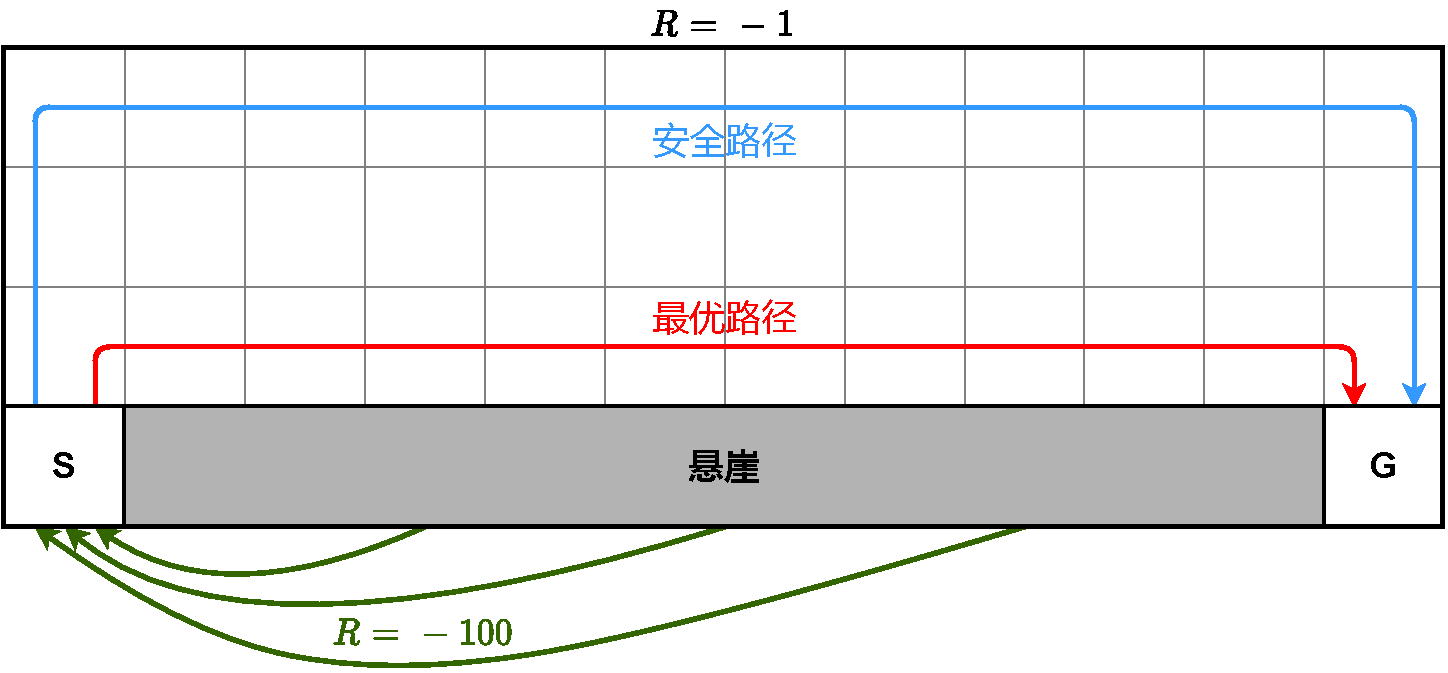
\includegraphics[width=\textwidth]{figures/cliff-env.pdf}
\caption{Cliff-Walking实验环境示意图}
\label{fig:cliff-env}
\end{figure}


为了直观理解双层经验重放的潜在好处,我们先设计了一组简单环境下的实验,引入了Cliff-Walking环境(如图~\ref{fig:cliff-env}~所示)。在该环境由$4\times 12$个方格组成,每次只能由一个方格移动到另一个相邻方格,并获得$R=-1$的反馈值,任务目标是从起始状态S出发,以尽可能快的速度到达终点状态G。如果智能体在行动过程中进入灰色的悬崖区域,则会直接返回初始状态S并得到$R=-100$的反馈值。显然,在Cliff-Walking环境下只存在唯一的最优路径,如图中的红线所示。然而,这条最优路径也是最危险的路径。如果算法在早期阶段效率不高,随时可能不小心从最优路径进入悬崖,造成较大的惩罚,从而影响算法的收敛性。在该环境下算法样本效率的提升会显著改善训练曲线的收敛速度。

我们使用优先经验算法(PER)作为基线进行测试,并设计了一个双层回放池的优先经验回放算法。表~\ref{tab:cliff-stats}~的实验结果显示了在Cliff-Walking环境下使用单层或双层重放缓冲区的PER算法统计结果。这些指标代表了智能体落入悬崖区的概率以及平均收益。每次实验的运行由3组随机种子生成,每次实验需要2000步。统计结果表明,用双层经验重放法训练的策略落入悬崖区的次数较少,在评估过程中表现出更好的稳健性。可以看出,当使用双层回放池时,PER算法的表现比单层回放缓冲器的整体表现要好。

\begin{figure}[t]
\centering
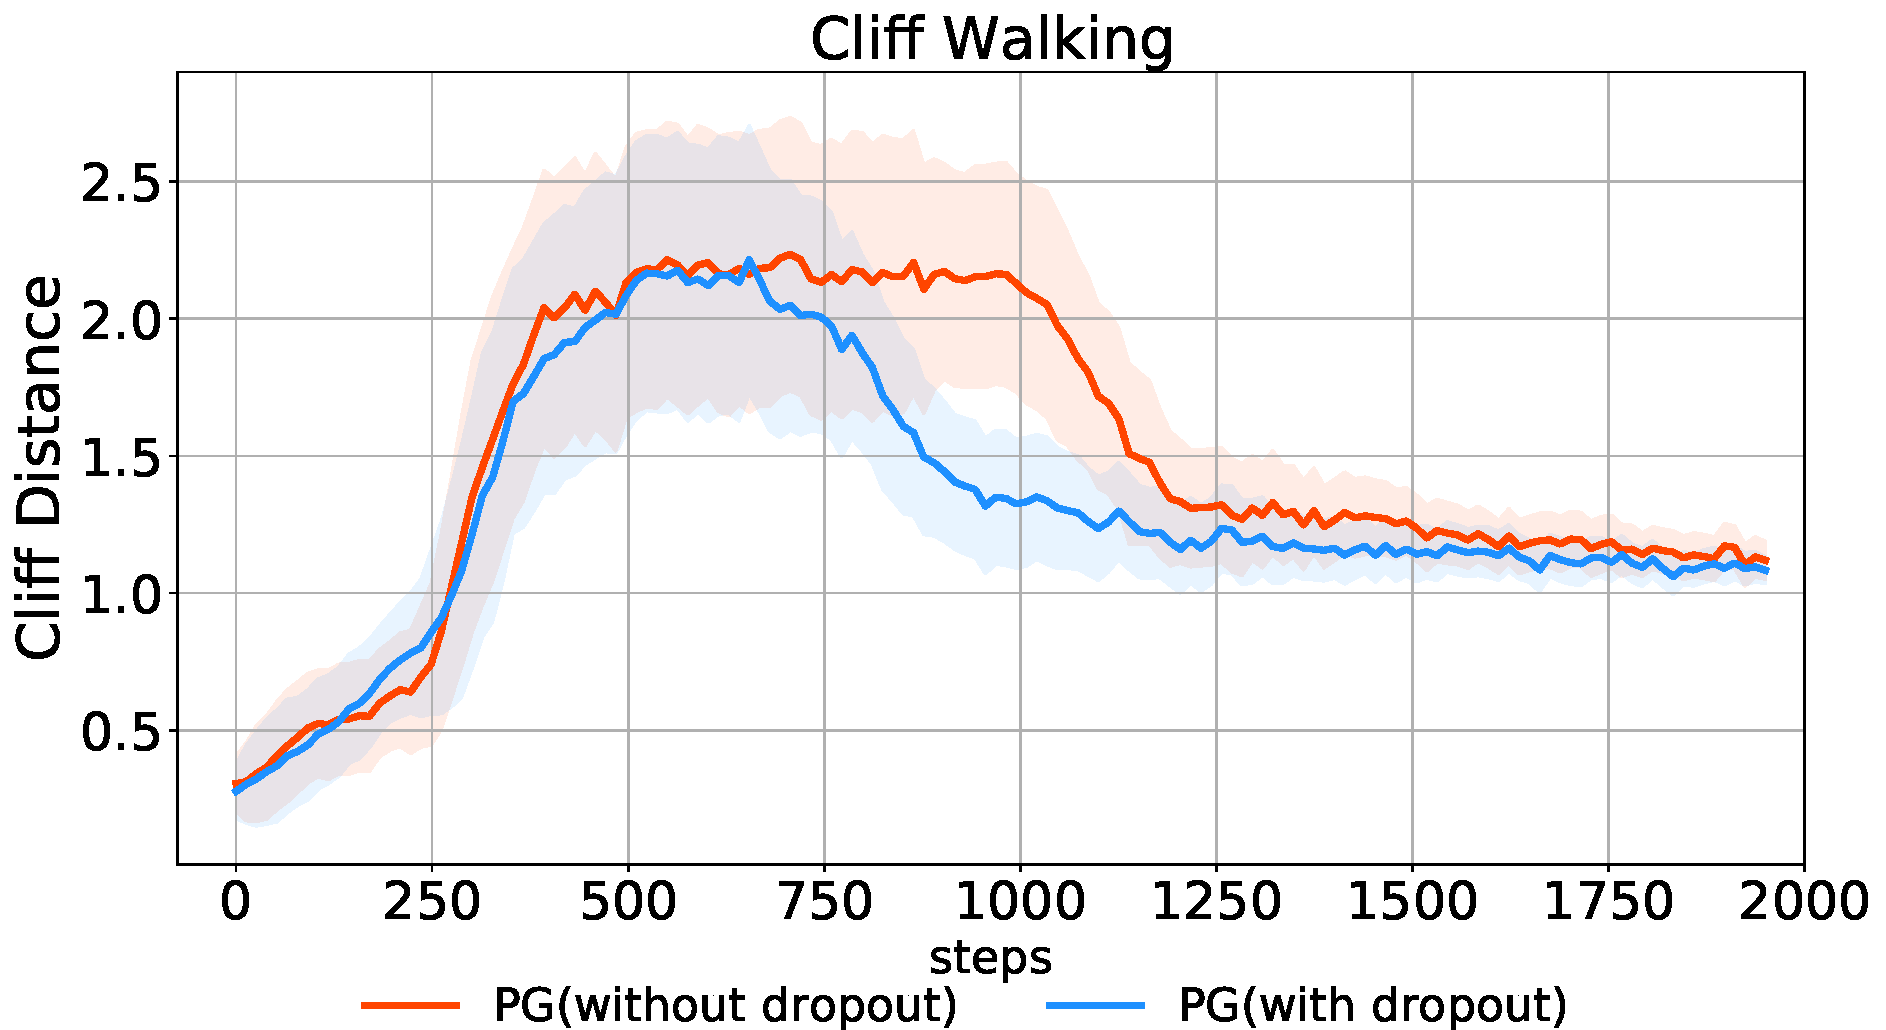
\includegraphics[width=\textwidth]{figures/cliffwalking.pdf}
\caption{Cliff-Walking实验结果曲线}
\label{fig:cliff-dis}
\end{figure}

\begin{table}[ht]
\centering
\begin{tabular}{l|l|l|l|l|l} 
\toprule
                                                    & Layer  & Seed 1           & Seed 2           & Seed 3           & Avg.              \\ 
\hline
\multirow{2}{*}{$P_\text{mean}(\text{Fail})$~ (\%)} & single & 0.645            & 0.678            & 0.611            & 0.645             \\ 
\cline{2-6}
                                                    & double & \textbf{0.357}   & \textbf{0.332}   & \textbf{0.312}   & \textbf{0.335}    \\ 
\hline
\multirow{2}{*}{$P_\text{std}(\text{Fail})$~ (\%)}  & single & 0.294            & 0.318            & 0.337            & 0.316             \\ 
\cline{2-6}
                                                    & double & \textbf{0.201}   & \textbf{0.197}   & \textbf{0.185}   & \textbf{0.194}    \\ 
\hline
\multirow{2}{*}{$R_\text{mean}$}                    & single & -13.258          & \textbf{-13.179} & -14.188          & -13.542           \\ 
\cline{2-6}
                                                    & double & \textbf{-12.978} & -13.205          & \textbf{-13.189} & \textbf{-13.124}  \\ 
\hline
\multirow{2}{*}{$R_\text{std}$}                     & single & 4.038            & 3.971            & 3.862            & 3.957             \\ 
\cline{2-6}
                                                    & double & \textbf{2.225}   & \textbf{2.378}   & \textbf{2.804}   & \textbf{2.469}    \\
\bottomrule
\end{tabular}
\caption{Result of Cliff Walking}
\label{tab:cliff-stats}
\end{table}

图~\ref{fig:cliff-dis}~展示了使用单层优先经验回放(红线)和双层优先经验回放(蓝线)在Cliff-Walking环境上训练时智能体距离悬崖边缘的距离。如图中训练曲线所示,原始PER算法中的智能体倾向于从远离悬崖的安全路径进行探索,直到它获得足够的信息来慢慢接近最优路径。相比之下,具有双层经验回放的PER算法能够更快地学习,并且能够更有把握地提前接近危险区域,从而更好地收敛到最优路径。可以看出使用了双层经验回放的算法可以更快的选择接近悬崖的最优路径,说明了DPER算法能够有效地提升学习速度,增加样本利用效率。

\subsection{Mujoco环境实验设计与分析}

\begin{figure}[t]
    \centering
    \subcaptionbox{Hopper}{
        \centering
        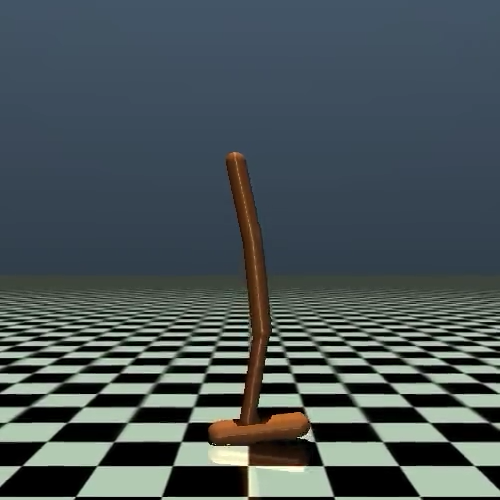
\includegraphics[width=0.48\textwidth]{figures/hopper.png}
        \label{fig:hopper}
    }
    \subcaptionbox{Walker}{
        \centering
        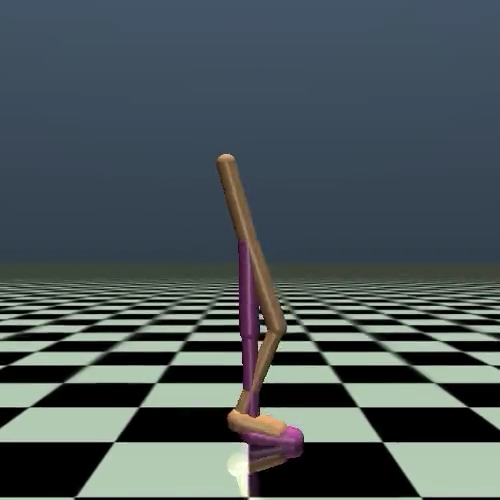
\includegraphics[width=0.48\textwidth]{figures/walker.png}
        \label{fig:walker}
    }
    \\
    \subcaptionbox{HalfCheetah}{
        \centering
        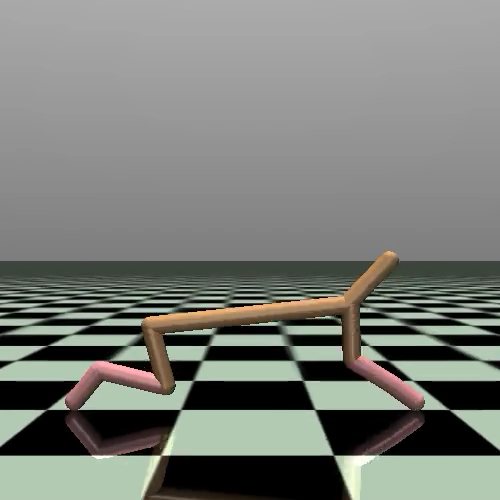
\includegraphics[width=0.48\textwidth]{figures/cheetah.png}
        \label{fig:cheetah}
    }
    \subcaptionbox{Ant}{
        \centering
        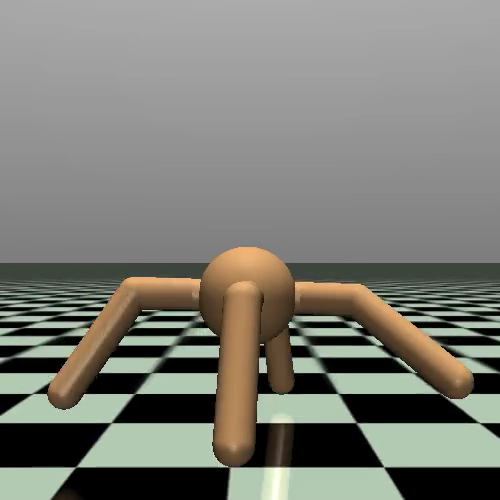
\includegraphics[width=0.48\textwidth]{figures/ant.png}
        \label{fig:ant}
    }
    \caption{实验所使用的四种仿真Mujoco环境示意图}
    \label{fig:env-figures}
\end{figure}

为了更细致地分析DPER算法的具体效果,我们选用了OpenAI-Gym库中的经典Mujoco仿真环境\cite{todorov2012mujoco}用于进一步的验证实验。具体地,我们选择了Mujoco下的Hopper,Walker,HalfCheetah和Ant这四个环境,他们都是验证智能体在连续动作条件下决策性能的常用测试环境,这四个环境的具体测试任务如下描述。

\begin{itemize}
    \item \textbf{Hopper}: 控制一个单腿机器人尽可能快地向前行走。
    \item \textbf{Walker2d}: 控制一个双腿机器人尽可能快地往前行走。
    \item \textbf{HalfCheetah}: 控制一个双腿爬行机器人尽可能快地向前行走。
    \item \textbf{Ant}: 控制一个四腿爬行机器人尽可能快地向前行走。
\end{itemize}

在本实验中,我们关于样本效率对比了多个基线方法,将基于模型的强化学习算法中的代表算法MBPO\cite{janner2019trust},以及它与PER \cite{schaul2016prioritized}的结合MBPO+PER进行了对比实验。在不同环境的实验中所使用的参数设定如表~\ref{tab:parameters}所示。

\begin{figure}[t]
  \centering
  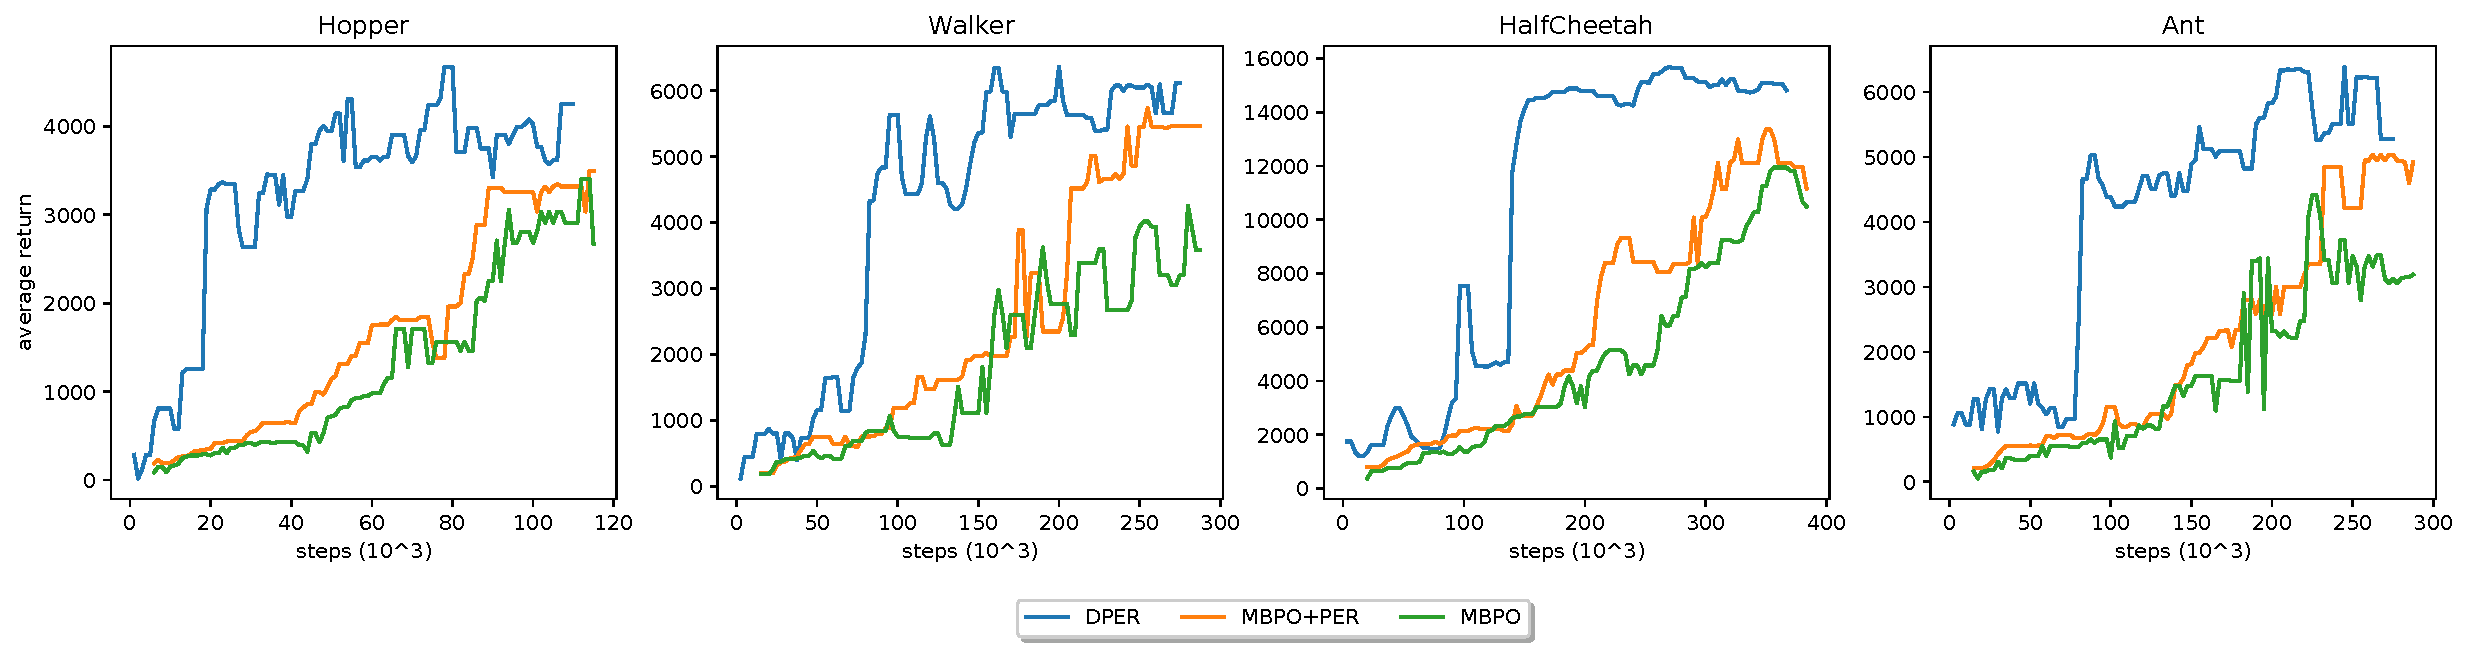
\includegraphics[width=\textwidth]{figures/dler.pdf}
  \caption{DPER算法与其他基线算法在不同环境下的训练曲线}
  \label{fig:dper-performance}
\end{figure}

\begin{table}[ht]
\centering
\begin{tabular}{c|c|c|c|c|c} 
\toprule
Env         & Epochs & $\alpha$ & \begin{tabular}[c]{@{}l@{}}buffer\\size\end{tabular} & \begin{tabular}[c]{@{}l@{}}env steps\\per epoch\end{tabular} & \begin{tabular}[c]{@{}l@{}}model steps\\per epoch\end{tabular}  \\ 
\hline
Hopper      & 120    & 0.2      & $10^5$                                              & 1000                                                         & 100                                                             \\ 
\hline
Walker      & 300    & 0.2      & $10^5$                                              & 1000                                                         & 100                                                             \\ 
\hline
HalfCheetah & 400    & 0.2      & $10^5$                                              & 1000                                                         & 200                                                             \\ 
\hline
Ant         & 300    & 0.2      & $10^5$                                              & 1000                                                         & 100                                                             \\
\bottomrule
\end{tabular}
\caption{DPER算法验证实验所使用的参数设定}
\label{tab:parameters}
\end{table}

具体而言,我们在Hopper环境运行了120轮循环,每轮循环包含1000步更新;相对应地,我们在Walker环境运行了300轮循环$\times$1000步;在HalfCheetah环境运行率400轮循环$\times$1000步;在Ant环境运行了300轮循环$\times$1000步。环境模型所使用的神经网络结构为$4\times 200$多层感知机(MLP)结构,这些模型在学习后均被用于预测未来100步的状态转移过程。所有实验中,DPER算法结构的第一层经验回放池大小均设为$10^5$,第二层经验回放池大小比例使用参数$\alpha=0.2$进行控制。在这些参数设定下,最终的训练曲线如图~\ref{fig:dper-performance}所示。所有曲线均由5组不同随机种子实验计算均值得到。根据图中结果可以看出,DPER算法在四种环境下的样本利用效率均超越了作为对比的MBPO算法和MBPO+PER算法,验证了基于双层缓存的优先经验回放算法在样本利用效率上的提升效果。

为了进一步确定DPER算法中参数$\alpha$的取值,我们还进行了一组参数实验,实验结果如表~\ref{tab:dper-ablation}所示。在该表中,我们对$\alpha$在区间$[0,0.5]$上分别进行了5组随机数种子实验,并计算了平均返回值,该指标越高,说明该参数在相应环境下能取得最优效果。可以看出,当$\alpha$取值为0.2时,DPER算法在Hopper、Walker、Ant环境上取得了最优的平均返回值,当$\alpha$取值为0.3时,DPER算法在HalfCheetah环境上取得了最优的平均返回值。基于上述结果可知,当$\alpha\in[0.2,0.3]$时,DPER算法能达到最优性能。

\begin{table}[ht]
\centering

\begin{tabular}{c|c|c|c|c|c|c} 
\toprule[2pt]
$\alpha$                           & 0       & 0.1     & 0.2             & 0.3              & 0.4     & 0.5      \\ 
\hline
$R_\text{avg}(\text{Hopper})$      & 3985.4  & 4057.1  & \textbf{4166.2} & 4030.7           & 3864.5  & 3796.5   \\ 
\hline
$R_\text{avg}(\text{Walker})$      & 5738.2  & 5943.4  & \textbf{6083.8} & 6008.1           & 5882.9  & 5694.4   \\ 
\hline
$R_\text{avg}(\text{HalfCheetah})$ & 15479.5 & 15630.1 & 15879.2         & \textbf{16036.1} & 15640.4 & 15038.1  \\ 
\hline
$R_\text{avg}(\text{Ant})$         & 5975.2  & 6023.5  & \textbf{6249.8} & 6199.5           & 6047.1  & 5926.3   \\
\bottomrule[2pt]
\end{tabular}

\caption{DPER算法参数对比实验结果}
\label{tab:dper-ablation}
\end{table}

\section{本章小结}

本章主要介绍了针对强化学习的样本利用效率问题所提出了基于双层缓存的优先经验回放算法(Double-layer Prioritized Experience Replay,DPER)。DPER算法通过双层经验回放池的设计,在添加的第二层经验回放池中以更慢的速率全局空间的经验样本进行回放缓存,提高了经验回放样本在整体样本空间中的有效覆盖率,加速了策略学习速度,最终实现了算法样本利用效率的提升。在CliffWalking和Mujoco中的Hopper、Walker2d、HalfCheetah、Ant仿真环境下均验证了DPER算法在样本利用效率的提升效果。
% !TeX root = ../main.tex

\chapter{基于模型集成的筛选规划算法}\label{chap:mbdp}

基于第~\ref{chap:background}~章中介绍的条件风险价值(CVaR)的思想,我们可以类似的在强化学习经验回放样本池中加入这一设计,将更低奖励反馈的样本加以更多的学习,而对过高奖励反馈的样本进行适当的筛选和丢弃,确保强化学习算法所学策略能够更稳定地处理高风险状态。

\section{MBDP算法描述与设计}

尽管在CVaR条件风险价值的思路下可以实现鲁棒性的提升,但是显然易见的是筛选丢弃样本的做法会损失一部分性能。为此,我们提出了基于模型集成的筛选规划算法(Model-Based Dropout Planning,MBDP),在做到提升算法鲁棒性的同时维持原有的算法性能。

\subsection{环境模型的集成学习与筛选}\label{sec:model-method}

传统的不确定性环境建模和集成方法,虽然已经能够较好地模拟真实复杂环境并且捕捉到环境的不确定性 \cite{duan2007multi},但并不能很好地控制模拟的精准程度,本论文在不确定性环境建模的基础上,结合传统集成学习的方法,设计了模型的集成和筛选机制。

具体地,首先训练学习一组环境模型集合$\{\mathcal{M}_{\phi_1},\mathcal{M}_{\phi_2},\ldots\}$,集合中每一个环境模型都是一个概率神经网络,其输出$\mu_{\phi_i},\sigma_{\phi_i}$构成高斯分布$\mathcal{N}(\mu_{\phi_i}(s,a),\sigma_{\phi_i}(s,a))$,环境模型对于下一时刻的状态预测则服从该分布,即
\begin{equation}
    s^\prime \sim \mathcal{M}_{\phi_i}(s,a) = \mathcal{N}(\mu_{\phi_i}(s,a),\sigma_{\phi_i}(s,a))
\end{equation}
在训练环境模型的同时,根据真实环境中采样得到的真实样本$(S,A)$,可以计算并记录模型的期望偏差:
\begin{equation}
    \mathrm{bias}(\phi_i) = \underset{S,A\sim \pi,\mathcal{P}}{\mathbb{E}}\|\mathcal{M}_{\phi_i}(S,A)-\mathcal{P}(S,A)\|
\end{equation}
其中$\|\cdot\|$是状态空间$\mathcal{S}$上的范数距离,该式的含义为所训练的环境模型$\mathcal{M}$与真实环境$\mathcal{P}$之间的范数意义距离。在上述模型集合的基础上,首先根据所计算的$\mathrm{bias}(\phi_i)$大小进行升序重排,并设定一个概率参数$\beta\in(0,1]$,筛选出$\mathrm{bias}$在$\beta$分位数以前的模型,保留得到筛选后的模型集合$\mathcal{M}^\beta = \{\mathcal{M}_{\phi_1},\mathcal{M}_{\phi_2},\ldots,\mathcal{M}_{\phi_{N_\beta}}\}$,其中$N_\beta$是前面所描述的升序排序后的集合索引$\left\{1,2,\ldots,N_\beta,\ldots\right\}$中的$\beta$分位数。

需要注意的是,用于集成的不确定性模型集合并不是$\mathrm{bias}$越小越好,过小的$\mathrm{bias}$可能意味着过拟合的环境模型。参数$\beta$的重要用处是可以动态地调整模型集合的整体精确性,它能与下一节将介绍的参数$\alpha$协作调整强化学习的收益性能与鲁棒性。

\subsection{环境模型的数据生成与筛选}\label{sec:rollout-method}

传统的基于模型的强化学习算法在得到环境模型后,往往是以期望收益为目标进行最大化优化,但是期望意义下的最优并不意味着在任意环境下都能有优秀的表现,在实际部署策略的时候,当面临一些受干扰的信息不足的状态,策略容易做出一些不合理甚至危险的决策,导致强化学习在实际部署中不稳定。为了解决这一问题,本论文提出了一种主动关注较坏情况的样本筛选机制,适当延缓强化学习训练速度,提升决策策略的鲁棒性。

具体地,基于上一节得到的$\mathcal{M}^{\beta}$模型集合,在每一步都随机抽取一个模型$\mathcal{M}_{\phi_i}\in\mathcal{M}^\beta$,然后使用该模型进行下一时刻的状态预测,即$s_{t+1}\sim \mathcal{M}_{\phi_t}(s_t,a_t), \phi_t\in\Phi_\beta$,这样的一组状态和动作组成模拟样本$x=\left(s_{t+1},s_t,a_t\right)$,填入缓存池,然后相似地以一个概率参数$\alpha\in(0,1]$进行筛选,从中挑选出反馈奖励值相对较低的样本,得到一个筛选后的$\alpha$分位数样本集合
\begin{equation}\label{def:batch-alpha-beta}
    \mathcal{B}_\alpha^{\pi,\mathcal{M}^\beta}=\left\{x|x\in\mathcal{B}^{\pi,\mathcal{M}^\beta},r(x|s)\leq r_{1-\alpha}(\mathcal{B}^{\pi,\mathcal{M}^\beta}|s), \forall s \in \mathcal{S}\right\},
\end{equation}
其中$\mathcal{B}^{\pi,\mathcal{M}^\beta}=\left\{x|x\triangleq\left(s_{t+1},s_t,a_t\right)\sim\pi,\mathcal{M}^\beta\right\}$, $r_{1-\alpha}(\mathcal{B}^{\pi,\mathcal{M}^\beta}|s)$ 是缓存池 $\mathcal{B}^{\pi,\mathcal{M}^\beta}$的$100\times(1-\alpha)$分位数。

\subsection{算法描述与整体框架}\label{sec:mbdp-description}

\begin{figure}[t]
\centering
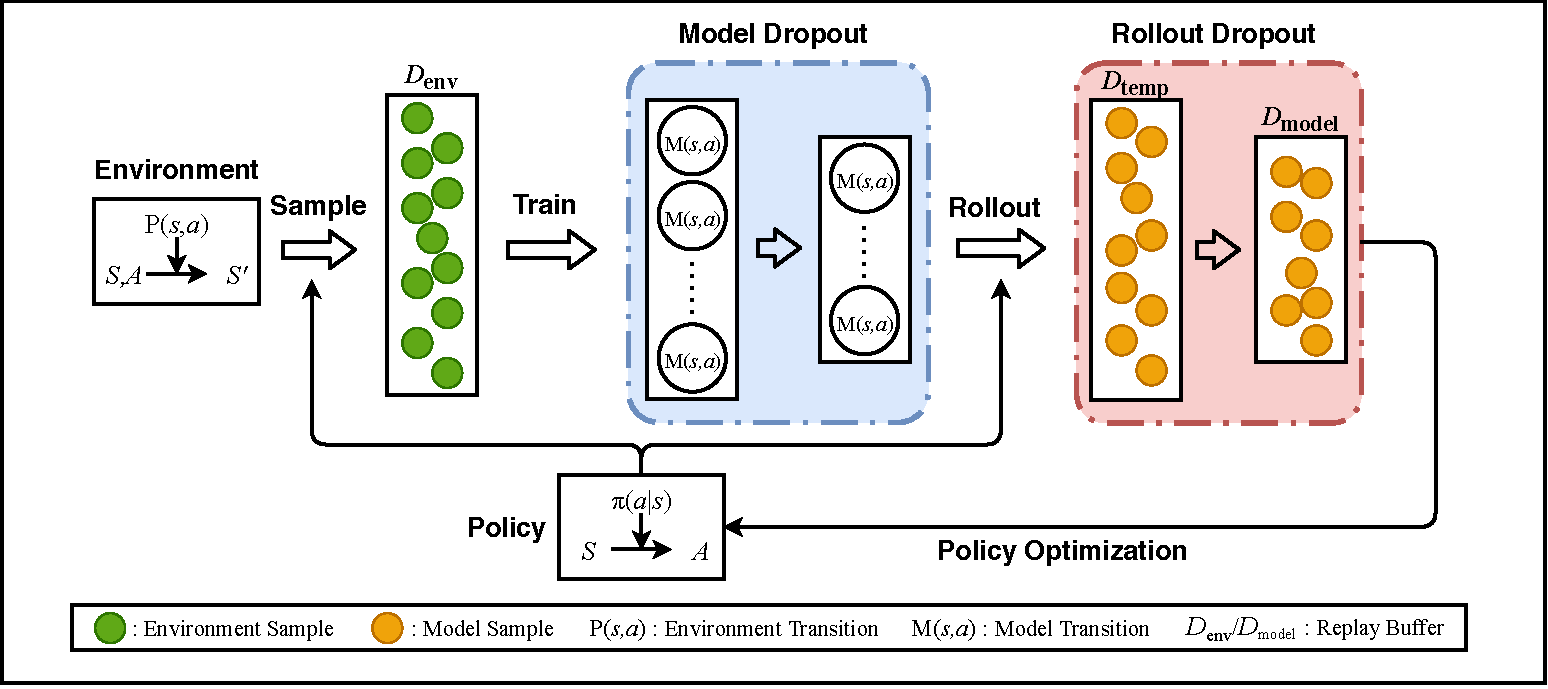
\includegraphics[width=\textwidth]{figures/mbdp.pdf}
\caption{基于模型集成的筛选规划算法示意图}
\label{fig:mbdp-structure}
\end{figure}

\begin{algorithm}[t]
\caption{基于模型集成的筛选规划算法 (\textbf{MBDP})}
\label{algo:our-method}
\begin{algorithmic}
\STATE 初始化超参数、策略 $\pi_\theta$、环境经验回放池 $\mathcal{D}_{\mathrm{env}}$、模型经验回放池 $\mathcal{D}_{\mathrm{model}}$\\
\FOR{$N_\mathrm{epoch}$ 迭代次数}
    \STATE 在环境中使用决策策略 $\pi_\theta$采取行动动作
    \STATE 将样本加入 $\mathcal{D}_{\mathrm{env}}$\\
    \FOR{$N_\mathrm{train}$ 迭代次数}
        \STATE  在收集的数据集$\mathcal{D}_{\mathrm{env}}$上训练概率模型$\mathcal{M}$\\
        \STATE 根据模型偏差$\mathrm{bias}({\phi_i})$构建模型子集 $\mathcal{M}^\beta = \{\mathcal{M}_{\phi_1},\ldots,\mathcal{M}_{\phi_{N_{1-\beta}}}\}$\\
        \FOR{$t=1,2,\ldots ,T$}
            \STATE 从 $\mathcal{M}^\beta$ 中随机抽选模型$\mathcal{M}_{\phi_t}$\\
            \STATE 在模型$\mathcal{M}_{\phi_t}$ 上使用策略$\pi_\theta$,生成样本$x=\left(s_{t+1},s_t,a_t\right)$ \\
            \STATE 将样本填入缓存回放池 $\mathcal{B}^{\pi,\mathcal{M}^\beta}$\\
        \ENDFOR
        \STATE 根据状态$s, \forall s\in\mathcal{S}$分组后计算$100\times(1-\alpha)$分位数,得到 $r_{1-\alpha}(\mathcal{B}^{\pi,\mathcal{M}^\beta}|s)$\\
        \FOR{$x\in \mathcal{B}^{\pi,\mathcal{M}^\beta}$}
            \IF{$r(x)\leq r_{1-\alpha}(\mathcal{B}^{\pi,\mathcal{M}^\beta}|s_t)$}
                \STATE 将 $x$ 填入 $\mathcal{D}_{\mathrm{model}}$
            \ENDIF
        \ENDFOR
    \ENDFOR
    \STATE 在$\mathcal{D}_{\mathrm{model}}$上优化$\pi_\theta$: $\theta\leftarrow \theta - \lambda\nabla_\theta J_\theta(\mathcal{D}_{\mathrm{model}})$
\ENDFOR
\end{algorithmic}
\end{algorithm}


由于在强化学习中模拟误差越小,算法的收敛性能则越好,观察公式(\ref{eq:MBDP-bound})中的误差上界$D_{\alpha,\beta}(\mathcal{M})$可知,强化学习的算法性能与参数$\alpha$成反比,与参数$\beta$成正比,又根据\ref{sec:model-method}节和\ref{sec:rollout-method}节的介绍可知,策略的鲁棒性显然与参数$\alpha$成正比,与参数$\beta$成反比,恰好与前面的作用效果相反。因此,本论文可以动态性地调整参数$\alpha,\beta$来取得算法性能和最终策略鲁棒性之间的平衡,从而得到不同属性的强化学习决策策略:

\begin{itemize}
    \item 平衡的决策策略:将参数$\alpha$和$\beta$调整为适中大小的概率值,适用于一般的普通环境;
    \item 收益性能较高的决策策略:将参数$\alpha$调整为较小的概率值,$\beta$调整为较大的概率值,适用于相对稳定的环境;
    \item 鲁棒性较好的决策策略:将参数$\alpha$调整为较大的概率值,$\beta$调整为较小的概率值,适用于干扰较大的环境。
\end{itemize}

基于~\ref{sec:model-method}~节和~\ref{sec:rollout-method}~节中提出的改进方案思路,将其整合进传统的基于模型的强化学习算法框架,得到改进的算法,算法整体框架如图\ref{fig:mbdp-structure}所示。MBDP算法首先通过与环境交互产生样本,用于训练概率模型并集成模拟,然后经过集成模型筛选模块生成模拟数据,再由模拟数据筛选模块生成处理后的模拟样本,最终将更新的模拟样本提供给策略优化公式对策略$\pi(a|s)$进行优化,并进行下一轮迭代。MBDP算法的主要流程如算法~\ref{algo:our-method}~所示。

\section{算法理论分析}

记在环境$\mathcal{P}$下,使用策略$\pi$进行交互所得的标准状态价值函数为
\begin{equation}\label{def:eta-s}
    {V}^{\pi,\mathcal{P}}(s) = \underset{\{a_0,s_1,\ldots\} \sim \pi,\mathcal{P}}{\mathbb{E}}\left[\sum_{t=0}^\infty\gamma^t r(s_t,a_t)\mid s_0=s\right].
\end{equation}

为便于分析,使用${V}^{\pi,\mathcal{P}}$表示基于随机初始状态的期望收益:
\begin{equation}\label{def:eta-expectation}
    {V}^{\pi,\mathcal{P}} = \underset{s_0\in\mathcal{S}}{\mathbb{E}} \left[{V}^{\pi,\mathcal{P}}(s_0)\right].
\end{equation}

可定义在MBDP方法中缓存池里的模拟样本构成的期望收益为${V}^{\pi,\mathcal{M}_\phi}_\alpha$:
\begin{equation}\label{def:eta-beta}
    {V}^{\pi,\mathcal{M}_\phi}_\alpha=\mathbb{E}\left[{\sum}_{\{s_0,a_0,\ldots\} \sim\mathcal{B}_\alpha^{\pi,\mathcal{M}_\phi}}\left[\gamma^t r(s_t,a_t)\right]\right].
\end{equation}

本论文可以证明,加入样本筛选机制后的模拟期望收益,与真实环境中期望收益的差异为一个受参数$\beta$控制的上界,如定理 \ref{the:beta-drop-bound} 所述。

\begin{theorem}\label{the:beta-drop-bound}

记$R_{m}$为奖励函数$r(s,a)$的上确界, 即 $R_{m}=\underset{s\in\mathcal{S},a\in\mathcal{A}}{\sup}r(s,a)$,在环境模型$\mathcal{M}_\phi$上使用样本筛选机制后,所得期望收益与真实环境中期望收益的差异值存在误差上界:
\begin{equation}
    |{V}_\alpha^{\pi, \mathcal{M}_{\phi}} - {V}^{\pi,\mathcal{M}_{\phi}}| \leq \frac{\alpha(1+\alpha)}{(1-\alpha)(1-\gamma)}\mathrm{R_{m}} \triangleq \epsilon_\alpha
\label{eq:eps-beta}
\end{equation}
\end{theorem}

定理~\ref{the:beta-drop-bound}的重要意义是,即使筛选掉一批模拟样本,环境模型给出的模拟数据仍具备一定的可靠性,该可靠性由概率参数$\alpha$控制。该定理的证明如下。

\begin{proof}


首先可以证明,对于两个不相交的集合 $A$ 和 $B$($A\cap B=\varnothing$) ,满足下列关系式
\begin{equation}
    \mathbb{E}_{A\cup B}\left[X\right] = \mathbb{E}_A\left[X\right]\cdot\mathrm{P}\left(A\right)+\mathbb{E}_B\left[X\right]\cdot\mathrm{P}\left(B\right)
\end{equation}
基于上述性质,可以计算得到
\begin{align}
    &\mathbb{E}\left[{\sum}_{s_0\in\mathcal{S},\{a_0,s_1,\ldots\} \sim\pi,\mathcal{M}_\phi}\left[\gamma^t r(s_t,a_t)\right]\right] \\
    &= (1-\alpha)\cdot \mathbb{E}\left[{\sum}_{\{s_0,a_0,\ldots\} \sim\mathcal{B}_\alpha^{\pi,\mathcal{M}_\phi}}\left[\gamma^t r(s_t,a_t)\right]\right] + \alpha\cdot\mathbb{E}\left[{\sum}_{\{s_0,a_0,\ldots\} \not\sim\mathcal{B}_\alpha^{\pi,\mathcal{M}_\phi}}\left[\gamma^t r(s_t,a_t)\right]\right]
\end{align}
根据定义 (\ref{def:eta-s}), (\ref{def:eta-expectation}) 和 (\ref{def:eta-beta}),我们可以得到
\begin{align}
{V}^{\pi,\mathcal{M}_\phi}_\alpha&=\mathbb{E}\left[{\sum}_{\{s_0,a_0,\ldots\} \sim\mathcal{B}_\alpha^{\pi,\mathcal{M}_\phi}}\left[\gamma^t r(s_t,a_t)\right]\right]\\
&=\frac{1}{1-\alpha}\mathbb{E}\left[{\sum}_{s_0\in\mathcal{S},\{a_0,s_1,\ldots\} \sim\pi,\mathcal{M}_\phi}\left[\gamma^t r(s_t,a_t)\right]\right]-\notag\\
&\frac{\alpha}{1-\alpha}\mathbb{E}\left[{\sum}_{\{s_0,a_0,\ldots\} \not\sim\mathcal{B}_\alpha^{\pi,\mathcal{M}_\phi}}\left[\gamma^t r(s_t,a_t)\right]\right]\\
&=\frac{1}{1-\alpha}\underset{s\in{\mathcal{S}}}{\mathbb{E}}\left[{V}^{\pi,\mathcal{M}_\phi}(s)\right]-\frac{\alpha}{1-\alpha}\mathbb{E}\left[{\sum}_{\tau \not\sim\mathcal{B}_\alpha^{\pi,\mathcal{M}_\phi}}\left[\gamma^t r(s_t,a_t)\right]\right]\\
&=\frac{1}{1-\alpha}{V}^{\pi,\mathcal{M}_\phi}-\frac{\alpha}{1-\alpha}\mathbb{E}\left[{\sum}_{\tau \not\sim\mathcal{B}_\alpha^{\pi,\mathcal{M}_\phi}}\left[\gamma^t r(s_t,a_t)\right]\right]\label{proof:lem42p1}
\end{align}
其中 $\tau\triangleq\{s_0,a_0,\ldots\}$。根据定义 (\ref{def:batch-alpha-beta}) 以及  $\mathrm{R}_{m}=\underset{s\in\mathcal{S},a\in\mathcal{A}}{\sup}r(s,a)$,可得
\begin{align}
\mathbb{E}\left[{\sum}_{\tau \not\sim\mathcal{B}_\alpha^{\pi,\mathcal{M}_\phi}}\left[\gamma^t r(s_t,a_t)\right]\right] &\leq\int_{\tau\not\sim{\mathcal{B}_\alpha^{\pi,\mathcal{M}_\phi}}}\left[\sum_{t=0}^\infty\gamma^t \mathrm{R}_m\right]p(\tau)\mathrm{d}\tau\\
&=\left[\sum_{t=0}^\infty\gamma^t\right]\mathrm{R}_m\int_{\tau\not\sim{\mathcal{B}_\alpha^{\pi,\mathcal{M}_\phi}}}p(\tau)\mathrm{d}\tau\\
&= \frac{1}{1-\gamma}\mathrm{R}_m \int_{\tau\not\sim{\mathcal{B}_\alpha^{\pi,\mathcal{M}_\phi}}}p(\tau)\mathrm{d}\tau\\
&=\frac{\alpha}{1-\gamma}\mathrm{R}_m
\end{align}
与之相似地,我们可以得到
\begin{align}
V^{\pi,\mathcal{M}_\phi} = \mathbb{E}\left[{\sum}_{\tau \sim\mathcal{B}^{\pi,\mathcal{M}_\phi}}\left[\gamma^t r(s_t,a_t)\right]\right] &\leq\int_{\tau \sim\mathcal{B}^{\pi,\mathcal{M}_\phi}}\left[\sum_{t=0}^\infty\gamma^t \mathrm{R}_m\right]p(\tau)\mathrm{d}\tau\\
&=\left[\sum_{t=0}^\infty\gamma^t\right]\mathrm{R}_m\int_{\tau \sim\mathcal{B}^{\pi,\mathcal{M}_\phi}}p(\tau)\mathrm{d}\tau\\
&= \frac{1}{1-\gamma}\mathrm{R}_m \int_{\tau \sim\mathcal{B}^{\pi,\mathcal{M}_\phi}}p(\tau)\mathrm{d}\tau\\
&=\frac{1}{1-\gamma}\mathrm{R}_m
\end{align}
根据上述推导得到的两个不等式关系以及方程式 (\ref{proof:lem42p1}),可知
\begin{align}
|{V}_\alpha^{\pi, \mathcal{M}_{\phi}} - {V}^{\pi,\mathcal{M}_{\phi}}| &=  \left|\frac{\alpha}{1-\alpha}V^{\pi,\mathcal{M}_\phi}-\frac{\alpha}{1-\alpha}\mathbb{E}\left[{\sum}_{\tau \not\sim\mathcal{B}_\alpha^{\pi,\mathcal{M}_\phi}}\left[\gamma^t r(s_t,a_t)\right]\right]\right| \\
&\leq\frac{\alpha}{1-\alpha}\left(\left|V^{\pi,\mathcal{M}_\phi}\right|+\left|\mathbb{E}\left[{\sum}_{\tau \not\sim\mathcal{B}_\alpha^{\pi,\mathcal{M}_\phi}}\left[\gamma^t r(s_t,a_t)\right]\right]\right|\right)\\
&\leq \frac{\alpha}{1-\alpha}\left(\frac{1}{1-\gamma}\mathrm{R}_m+\frac{\alpha}{1-\gamma}\mathrm{R}_m\right) \\
&=\frac{\alpha(1+\alpha)}{(1-\alpha)(1-\gamma)}\mathrm{R_{m}} \label{eq:lem42}
\end{align}

\end{proof}

更进一步地,我们可以证明在同时加入模拟数据筛选模块和集成模型筛选模块后,所得到的策略期望价值仍然与真实环境下的策略收益存在一个可控的误差上界,并且该上界由筛选比例$\alpha$和$\beta$控制。

\begin{theorem}\label{the:MBDP-bound}

设 $K\geq 0$ 是一项常数。 在同时加入模拟数据筛选模块和集成模型筛选模块后所得到的策略期望价值 ${V}_\alpha^{\pi, \mathcal{M}^\beta}$,与真实环境$\mathcal{P}$下所能得到的期望策略价值 ${V}^{\pi, \mathcal{P}}$存在一个误差上界:
\begin{equation}
\left|{V}_\alpha^{\pi, \mathcal{M}^\beta}-{V}^{\pi, \mathcal{P}}\right|\leq D_{\alpha,\beta}(\mathcal{M})
\end{equation}
其中
\begin{equation}\label{eq:MBDP-bound}
D_{\alpha,\beta}(\mathcal{M})\triangleq\frac{(1-\beta)\gamma K}{1-\gamma}\epsilon_{\mathcal{M}}+\frac{\alpha(1+\alpha)(1-\beta)}{(1-\alpha)(1-\gamma)}\mathrm{R}_m
\end{equation}
并且
\begin{equation}\label{def:delta-M}
\epsilon_{\mathcal{M}}\triangleq\underset{\phi\in\Phi}{\mathbb{E}}\left[\underset{s,a\sim \pi,\mathcal{P}}{\mathbb{E}}\left[\left\|\mathcal{M}_\phi(s, a)-\mathcal{P}(s, a)\right\|\right]\right]
\end{equation}

\end{theorem}
为了证明上述定理,我们首先需要引入两个引理

\begin{lemma}\label{lem:proof-for-lem41}
定义
\begin{equation}\label{def:G-sa}
G^{\pi,\mathcal{M}}(s,a)=\underset{\hat{s}'\sim\mathcal{M}(\cdot|s,a)}{\mathbb{E}}{{V}^{\pi,\mathcal{M}}}(\hat{s}') - \underset{s'\sim\mathcal{P}(\cdot|s,a)}{\mathbb{E}}{{V}^{\pi,\mathcal{M}}}(s')
\end{equation}
对于任意策略 $\pi$ 和任意动态模型 $\mathcal{M},\mathcal{M}'$,存在如下关系式
\begin{equation}
{V}^{\pi,\mathcal{M}'} - {V}^{\pi,\mathcal{M}} = \frac{\gamma}{1-\gamma}\underset{S,A\sim\pi,\mathcal{M}}{\mathbb{E}}\left[G^{\pi,\mathcal{M}'}(S,A)\right]
\end{equation}
\end{lemma}

引理 \ref{lem:proof-for-lem41} 改写自Luo等人在其论文\cite{luo2018algorithmic}中提出的引理4.3。在该引理的基础上,本文进一步推导出如下的引理 \ref{lem:mb-bound}。

\begin{lemma}\label{lem:mb-bound}
设基于模型方法所能取得的价值函数 ${V}^{\pi,\mathcal{M}}$ 在状态空间$\mathcal{S}$上是Lipschitz连续的,并设$K$为 Lipschitz常数,。记$\mathcal{P}$表示真实环境的状态转移概率分布,则有如下的不等式关系:
\begin{equation}
\left|{V}^{\pi, \mathcal{M}}-{V}^{\pi, \mathcal{P}}\right| \leq\frac{\gamma}{1-\gamma}K\cdot\mathrm{bias}
\end{equation}
其中
\begin{equation}
\mathrm{bias} \triangleq \underset{s,a\sim \pi,\mathcal{P}}{\mathbb{E}}\left\|\mathcal{M}(s, a)-\mathcal{P}(s, a)\right\|
\end{equation}

\label{theo:mb-bound}
\end{lemma}

在引理 \ref{lem:mb-bound}中, 我们假设了关于估计模型$\mathcal{M}$的期望收益${V}^{\pi,\mathcal{M}}(s)$ 关于任意范数距离$\|\cdot\|$都是Lipschitz连续的,即
\begin{equation}\label{assum:lip}
    \left|{V}^{\pi,\mathcal{M}}(s)-{V}^{\pi,\mathcal{M}}(s^{\prime})\right| \leq K\left\|s-s^{\prime}\right\|, \forall s, s^{\prime} \in \mathcal{S}
\end{equation}
其中$K\in \mathbb{R}^+$ 是一个Lipschitz常数。该假设的意义是相近的状态应该拥有相似的价值估计,对于绝大多数场景而言,这一假设显然都是成立的。引理~\ref{lem:mb-bound}的证明如下:

\begin{proof}

根据$G^{\pi,\mathcal{M}}(s,a)$在公式(\ref{def:G-sa})的定义,以及假设 ${V}^{\pi,\mathcal{M}}(s)$ 满足 Lipschitz 连续性(\ref{assum:lip}), 我们可以得到

\begin{equation}\label{eq:G-leq}
|G^{\pi,\mathcal{M}}(s,a)|\leq K\|\mathcal{M}(s,a)-\mathcal{P}(s,a)\|
\end{equation}
可以证明
\begin{align}
\left|{V}^{\pi, \mathcal{M}}-{V}^{\pi, \mathcal{P}}\right| &= \frac{\gamma}{1-\gamma}\left|\underset{s,a\sim\pi,\mathcal{P}}{\mathbb{E}}\left[G^{\pi,\mathcal{M}}(s,a)\right]\right|\\
&\leq \frac{\gamma}{1-\gamma}\underset{s,a\sim\pi,\mathcal{P}}{\mathbb{E}}\left[\left|G^{\pi,\mathcal{M}}(s,a)\right|\right]\\
&\leq \frac{\gamma}{1-\gamma}\underset{s,a\sim\pi,\mathcal{P}}{\mathbb{E}}K\|\mathcal{M}(s,a)-\mathcal{P}(s,a)\|\\
&= \frac{\gamma}{1-\gamma}K\cdot\underset{s,a\sim\pi,\mathcal{P}}{\mathbb{E}}\|\mathcal{M}(s,a)-\mathcal{P}(s,a)\|\\
&\triangleq \frac{\gamma}{1-\gamma}K\cdot\mathrm{bias}
\end{align}

\end{proof}

定理~\ref{the:MBDP-bound}~的重要意义是,在加入模拟数据筛选模块和集成模型筛选模块后,模型给出的模拟数据与传统的模拟方式相比只存在一个可控的误差上界,对强化学习的训练带来的误差影响并不大,在该可控范围内,如前文对筛选机制的具体描述,本论文能够得到鲁棒性更好的决策策略。基于定理~\ref{the:beta-drop-bound}~和引理~\ref{lem:mb-bound}~,可证明定理~\ref{the:MBDP-bound}~,证明过程如下。

\begin{proof}

根据定理~\ref{the:beta-drop-bound}和引理~\ref{lem:mb-bound},首先可以证明

\begin{align}
\left|{V}_\alpha^{\pi, \mathcal{M}^\beta}-{V}^{\pi, \mathcal{P}}\right|&=\left|\int_{\Phi_\beta}{V}_\alpha^{\pi, \mathcal{M}_{\phi}}p(\phi)\mathrm{d}\phi-{V}^{\pi, \mathcal{P}}\right| \\
&=\left|\int_{\Phi_\beta}\left({V}_\alpha^{\pi, \mathcal{M}_{\phi}}-{V}^{\pi, \mathcal{P}}\right)p(\phi)\mathrm{d}\phi\right| \\
&\leq\int_{\Phi_\beta}\left|{V}_\alpha^{\pi, \mathcal{M}_{\phi}}-{V}^{\pi, \mathcal{P}}\right|p(\phi)\mathrm{d}\phi\\
&\leq\int_{\Phi_\beta}\left(\left|{V}^{\pi, \mathcal{M}_{\phi}}-{V}^{\pi, \mathcal{P}}\right|+\left|{V}_\alpha^{\pi, \mathcal{M}_{\phi}} - {V}^{\pi,\mathcal{M}_{\phi}}\right|\right)p(\phi)\mathrm{d}\phi\\
&= \int_{\Phi_\beta}\left|{V}^{\pi, \mathcal{M}_{\phi}}-{V}^{\pi, \mathcal{P}}\right|p(\phi)\mathrm{d}\phi+\int_{\Phi_\beta}\left|{V}_\alpha^{\pi, \mathcal{M}_{\phi}} - {V}^{\pi,\mathcal{M}_{\phi}}\right|p(\phi)\mathrm{d}\phi \label{proof:theo43p1}
\end{align}
对于公式 (\ref{proof:theo43p1})的第一部分,记
\begin{equation}
    \epsilon_{\mathcal{M}}\triangleq\underset{\phi\in\Phi}{\mathbb{E}}\left[\underset{s,a\sim \pi,\mathcal{P}}{\mathbb{E}}\left[\left\|\mathcal{M}_\phi(s, a)-\mathcal{P}(s, a)\right\|\right]\right]
\end{equation}
表示在模型$\mathcal{M}$和环境$\mathcal{P}$之间的一般性偏差。根据引理~\ref{lem:mb-bound},我们可以得到
\begin{align}
\int_{\Phi_\beta}\left|{V}^{\pi, \mathcal{M}_{\phi}}-{V}^{\pi, \mathcal{P}}\right|p(\phi)\mathrm{d}\phi &\leq \frac{\gamma K}{1-\gamma}\int_{\Phi_\beta}\underset{s,a\sim\pi,\mathcal{P}}{\mathbb{E}}\left[\left\|\mathcal{M}_\phi(s, a)-\mathcal{P}(s, a)\right\|\right]p(\phi)\mathrm{d}\phi\\
&\leq \frac{\gamma K}{1-\gamma}\left|\epsilon_{\mathcal{M}}\right|\int_{\Phi_\beta}\left|p(\phi)\right|\mathrm{d}\phi\\
&=\frac{(1-\beta)\gamma K}{1-\gamma}\epsilon_{\mathcal{M}} \label{proof:theo43p2}
\end{align}
对于公式 (\ref{proof:theo43p1})的第二部分, 根据定理~\ref{the:beta-drop-bound},我们可以证明
\begin{align}
\int_{\Phi_\beta}\left|{V}_\alpha^{\pi, \mathcal{M}_{\phi}} - {V}^{\pi,\mathcal{M}_{\phi}}\right|p(\phi)\mathrm{d}\phi&\leq \frac{\alpha(1+\alpha)}{(1-\alpha)(1-\gamma)}\mathrm{R}_m\int_{\Phi_\beta}p(\phi)\mathrm{d}\phi\\
&=\frac{\alpha(1+\alpha)(1-\beta)}{(1-\alpha)(1-\gamma)}\mathrm{R}_m \label{proof:theo43p3}
\end{align}
将上述结果代回公式 (\ref{proof:theo43p1}),可以得到
\begin{align}
\left|{V}_\alpha^{\pi, \mathcal{M}^\beta}-{V}^{\pi, \mathcal{P}}\right| &\leq \int_{\Phi_\beta}\left|{V}^{\pi, \mathcal{M}_{\phi}}-{V}^{\pi, \mathcal{P}}\right|p(\phi)\mathrm{d}\phi+\int_{\Phi_\beta}\left|\epsilon_\alpha\right|p(\phi)\mathrm{d}\phi\\
&\leq \frac{(1-\beta)\gamma K}{1-\gamma}\epsilon_{\mathcal{M}}+\frac{\alpha(1+\alpha)(1-\beta)}{(1-\alpha)(1-\gamma)}\mathrm{R}_m\\
&\triangleq D_{\alpha,\beta}(\mathcal{M})
\end{align}

\end{proof}

根据定理~\ref{the:MBDP-bound}中的的误差上界$D_{\alpha,\beta}(\mathcal{M})$分析可以得出结论,由于$D_{\alpha,\beta}(\mathcal{M})$与$\alpha$成正比,与$\beta$成反比,易知当$\alpha$增大或$\beta$减小时,该误差上界会被扩大,导致算法训练过程中的准确性下降,使得算法需要更长时间才能收敛,最终致使算法的样本效率降低。反之,若$\alpha$减小或$\beta$增大时,算法的样本效率则能得以提升。

由于MBDP算法作为基于模型的强化学习算法,可将其更新规则表示为如下的公式:
\begin{equation}
    \pi_{k+1}, \mathcal{M}^\beta_{k+1}=\underset{\pi_k, \mathcal{M}_k^\beta}{\arg\max}\left[{V}^{\pi_k, \mathcal{M}_k^\beta}-D_{\alpha,\beta}(\mathcal{M}^\beta_k)\right],
\label{eq:algo-equation}
\end{equation}
在该更新式的表达下,我们可以给出如下的定理
\begin{theorem}
更新公式(\ref{eq:algo-equation})每一步所得的策略部署在真实环境$\mathcal{P}$中时,其期望收益将会关于步数呈现单调递增趋势,即
\begin{equation}
    {V}^{\pi_{k+1}, \mathcal{P}}\geq {V}^{\pi_{k}, \mathcal{P}} + (\epsilon_{k+1} - \epsilon_\alpha) \triangleq {V}^{\pi_{k}, \mathcal{P}} + \eta,
\end{equation}
其中
\begin{equation}
    \epsilon_\alpha \triangleq |{V}_\alpha^{\pi, \mathcal{M}_{\phi}} - {V}^{\pi,\mathcal{M}_{\phi}}|   \leq \frac{\alpha}{1-\gamma}\mathrm{R_{m}}
\end{equation}
而$\epsilon_{k+1}$表示更新残差,记作
\begin{equation}
    \epsilon_{k+1} \triangleq {V}^{\pi_{k+1}, \mathcal{P}} - \left[{V}_{\alpha}^{\pi_{k+1}, \mathcal{M}_{k+1}^\beta} - D_{\alpha,\beta}(\mathcal{M}_{k+1}^\beta)\right].
\end{equation}
\label{prop:performance}
\end{theorem}

\begin{proof}

根据定理~\ref{the:MBDP-bound}, $\left|{V}_\alpha^{\pi, \mathcal{M}^\beta}-{V}^{\pi, \mathcal{P}}\right|\leq D_{\alpha,\beta}(\mathcal{M})$,可得
\begin{equation}\label{eq:prop44p1}
{V}^{\pi_{k+1}, \mathcal{P}} \geq {V}_{\alpha}^{\pi_{k+1}, \mathcal{M}_{k+1}^\beta}-D_{\alpha,\beta}(\mathcal{M}_{k+1}^\beta)
\end{equation}
由于不等式 (\ref{eq:prop44p1}) 的左边部分 ${V}^{\pi_{k+1}, \mathcal{P}}$ 比右边部分${V}_{\alpha}^{\pi_{k+1}, \mathcal{M}_{k+1}^\beta}-D_{\alpha,\beta}(\mathcal{M}_{k+1}^\beta)$大,我们可以将该不等式改写为一个带有残差项$\epsilon_{k+1}$的等式:
\begin{equation}\label{proof:prop44p1}
{V}^{\pi_{k+1}, \mathcal{P}} = {V}_{\alpha}^{\pi_{k+1}, \mathcal{M}_{k+1}^\beta}-D_{\alpha,\beta}(\mathcal{M}_{k+1}^\beta) + \epsilon_{k+1}
\end{equation}
其中
\begin{equation}
\epsilon_{k+1} \triangleq {V}^{\pi_{k+1}, \mathcal{P}} - \left[{V}_{\alpha}^{\pi_{k+1}, \mathcal{M}_{k+1}^\beta} - D_{\alpha,\beta}(\mathcal{M}_{k+1}^\beta)\right]
\end{equation}
根据更新规则 (\ref{eq:algo-equation}),可得
\begin{equation}\label{proof:prop44p2}
{V}_{\alpha}^{\pi_{k+1}, \mathcal{M}_{k+1}^\beta}-D_{\alpha,\beta}(\mathcal{M}_{k+1}^\beta) \geq {V}^{\pi_k,\mathcal{P}}-D_{\alpha,\beta}(\mathcal{P})
\end{equation}
由于
\begin{align}
\epsilon_{\mathcal{P}} &= \underset{\phi\in\Phi}{\mathbb{E}}\left[\underset{s,a\sim \pi,\mathcal{P}}{\mathbb{E}}\left[\left\|\mathcal{P}(s, a)-\mathcal{P}(s, a)\right\|\right]\right]\\
&=\underset{\phi\in\Phi}{\mathbb{E}}\left[0\right] = 0
\end{align}
可以证明
\begin{align}
D_{\alpha,\beta}(\mathcal{P}) &= \frac{(1-\beta)\gamma K}{1-\gamma}\epsilon_{\mathcal{P}}+\frac{\alpha(1+\alpha)(1-\beta)}{(1-\alpha)(1-\gamma)}\mathrm{R}_m\\
&=0+\frac{\alpha(1+\alpha)(1-\beta)}{(1-\alpha)(1-\gamma)}\mathrm{R}_m\\
&=\epsilon_\alpha \label{proof:prop44p3}
\end{align}
根据公式(\ref{proof:prop44p1}),(\ref{proof:prop44p2})和(\ref{proof:prop44p3}),
\begin{equation}
{V}^{\pi_{k+1}, \mathcal{P}}\geq {V}^{\pi_{k}, \mathcal{P}} + \left[\epsilon_{k+1} - \epsilon_\alpha\right]
\end{equation}
显然可知,更新残差项$\epsilon_{k+1}$在训练阶段远大于$\epsilon_\alpha$,因此满足 $\left[\epsilon_{k+1} - \epsilon_\alpha\right]\geq 0$,从而
\begin{equation}
{V}^{\pi_{k+1}, \mathcal{P}}\geq{V}^{\pi_{k}, \mathcal{P}}+0 
\end{equation}
最终证得
\begin{equation}
{V}^{\pi_{0}, \mathcal{P}} \leq \cdots \leq {V}^{\pi_{k}, \mathcal{P}} \leq {V}^{\pi_{k+1}, \mathcal{P}} \leq \cdots
\end{equation}

\end{proof}

上述的分析论证了MBDP算法在样本效率上能够确保策略收益随训练步数单调递增,下面对MBDP算法的鲁棒性进行分析论证。首先我们将鲁棒性定义为算法在受干扰环境下的期望性能。考虑一个干扰矩阵$\hat{\mathcal{P}}=\mathcal{P}_t \circ \delta_t$,其中$\delta_t\in\mathbb{R}^{\mathcal{S}\times\mathcal{A}\times\mathcal{S}}$为可积概率干扰,“$\circ$”为Hadamard乘积记号。根据公式(\ref{eq:def-cvar})中对$\mathrm{CVaR}(\cdot)$的定义,我们提出定理~\ref{the:robustness}~。

\begin{theorem}\label{the:robustness}
给定$\alpha\in(0,1)$以及干扰约束集合
\begin{equation}\label{eq:supp-perturbation}
    \Delta_\alpha \triangleq \left\{\delta_i\middle\vert\prod_{i=1}^{T}\delta_i(s_i\mid s_{i-1},a_{i-1})\leq \frac{1}{\alpha}, \forall s_i\in\mathcal{S}, a_i\in\mathcal{A}\right\}.
\end{equation}
存在如下关系
\begin{equation}\label{eq:return-cvar-rob}
    V_\alpha^{\pi,\mathcal{M}} = -\mathrm{CVaR}_\alpha\left(-V^{\pi,\mathcal{M}}\right)=\inf\limits_{\Delta_\alpha}\mathbb{E}_{\hat{\mathcal{P}}}\left[V^{\pi,\mathcal{M}}\right]
\end{equation}
\end{theorem}

\begin{proof}
根据 $\mathrm{CVaR}$ 的定义公式 (\ref{eq:def-cvar}) 和 $V_\alpha^{\pi,\mathcal{M}}$的定义公式
(\ref{def:eta-beta}),我们将奖励反馈取负值用于表示损失。此时可以证明
\begin{align}
\mathrm{CVaR}_\alpha(-V^{\pi,\mathcal{M}}) &= \mathbb{E}\left[-V^{\pi,\mathcal{M}}\mid -V^{\pi,\mathcal{M}} \geq \mathrm{VaR}_\alpha(-V^{\pi,\mathcal{M}})\right]\\
&=\mathbb{E}\left[-{\sum}_{\mathcal{B}^{\pi,\mathcal{M}}}\left[\gamma^t r(s_t,a_t)\right]\mid -{\sum}_{\mathcal{B}^{\pi,\mathcal{M}}}\left[\gamma^t r(s_t,a_t)\right] \geq \mathrm{VaR}_\alpha(-V^{\pi,\mathcal{M}})\right]\\
&=-\mathbb{E}\left[{\sum}_{\mathcal{B}^{\pi,\mathcal{M}}}\left[\gamma^t r(s_t,a_t)\right]\mid {\sum}_{\mathcal{B}^{\pi,\mathcal{M}}}\left[\gamma^t r(s_t,a_t)\right] \leq -\mathrm{VaR}_\alpha(-V^{\pi,\mathcal{M}})\right]
\end{align}
显然,上述公式中的条件 ${\sum}_{\mathcal{B}^{\pi,\mathcal{M}}}\left[\gamma^t r(s_t,a_t)\right] \leq -\mathrm{VaR}_\alpha(-V^{\pi,\mathcal{M}})$ 符合公式(\ref{def:batch-alpha-beta})的定义,即$\mathcal{B}_\alpha^{\pi,\mathcal{M}}$,因此,定理~\ref{the:robustness}的第一个等式得证。
\begin{equation}
-\mathrm{CVaR}_\alpha(-V^{\pi,\mathcal{M}}) = \mathbb{E}\left[{\sum}_{\mathcal{B}_\alpha^{\pi,\mathcal{M}}}\left[\gamma^t r(s_t,a_t)\right]\right] = V_\alpha^{\pi,\mathcal{M}}
\end{equation}
考虑到$\mathbb{E}_{\hat{\mathcal{P}}}[-V^{\pi,\mathcal{M}}]$,根据$\hat{\mathcal{P}}$的定义可知,
\begin{align}
    \mathbb{E}_{\hat{\mathcal{P}}}[V^{\pi,\mathcal{M}}] &= -\mathbb{E}_{\hat{\mathcal{P}}}[-V^{\pi,\mathcal{M}}]\\
    &= -\sum_{(s_0,\ldots,s_T)\in\mathcal{S}^{T+1}}\mathcal{P}_0(s_0)\delta_0(s_0)\prod_{t=1}^{T}\mathcal{P}_t(s_t\mid s_{t-1})\delta_t(s_t\mid s_{t-1})\cdot (-V^{\pi,\mathcal{M}})\\
    &= \sum_{(s_0,\ldots,s_T)\in\mathcal{S}^{T+1}}\mathcal{P}(s_0,\ldots,s_T)\delta_0(s_0)\prod_{t=1}^{T}\delta_t(x_t\mid x_{t-1})\cdot V^{\pi,\mathcal{M}}\\
    &\triangleq \sum_{(s_0,\ldots,s_T)\in\mathcal{S}^{T+1}}\mathcal{P}(s_0,\ldots,s_T)\delta(s_0,\ldots,s_T)\cdot V^{\pi,\mathcal{M}}
\end{align}
由于$\delta$ 为环境中的随机干扰,显然可知
\begin{equation}\label{eq:delta-exp}
    \mathbb{E}\left[\delta(s_0,\ldots,s_T)\right] = \sum_{(s_0,\ldots,s_T)\in\mathcal{S}^{T+1}}\mathcal{P}(s_0,\ldots,s_T)\delta(s_0,\ldots,s_T) = 1
\end{equation}
根据$\Delta_\alpha$ 的定义 (\ref{eq:supp-perturbation}),可以证明定理~\ref{the:robustness}的第二个等式
\begin{align}
    \inf\limits_{\Delta_\alpha}\mathbb{E}_{\hat{\mathcal{P}}}[V^{\pi,\mathcal{M}}] &= \inf\limits_{\delta(s_0,\ldots,s_T)\leq\frac{1}{\alpha}}\sum_{(s_0,\ldots,s_T)\in\mathcal{S}^{T+1}}\mathcal{P}(s_0,\ldots,s_T)\delta(s_0,\ldots,s_T)\cdot V^{\pi,\mathcal{M}}\\
    &=-\mathrm{CVaR}_\alpha(-V^{\pi,\mathcal{M}})\label{proof:cvar-eq}
\end{align}
上述的等式 (\ref{proof:cvar-eq}) 是由根据公式 (\ref{eq:delta-exp})和CVaR的表达性定理证明得到。

\end{proof}

\section{Mujoco环境实验设计与分析}

\begin{table}[ht]
\centering

\begin{tabular}{ccccccccc}
\toprule
  \begin{tabular}[c]{@{}c@{}}环境\end{tabular} &
  \begin{tabular}[c]{@{}c@{}}训练步数\end{tabular} &
  \begin{tabular}[c]{@{}c@{}}缓存大小\end{tabular} &
  \begin{tabular}[c]{@{}c@{}}策略更新\\步数\end{tabular} &
  \begin{tabular}[c]{@{}c@{}}模型更新\\步数\end{tabular} &
  $\alpha$ &
  $\beta$ &
  $\gamma$ &
  \begin{tabular}[c]{@{}c@{}}网络结构\end{tabular} \\
\midrule
Hopper      & 120000 & $10^5$ & 20 & 250 & 0.2 & 0.2 & 0.99 & \begin{tabular}[c]{@{}c@{}}MLP \\ ($4\times 200$)\end{tabular} \\
Walker    & 300000 & $10^5$ & 20 & 250 & 0.2 & 0.2 & 0.99 & \begin{tabular}[c]{@{}c@{}}MLP \\ ($4\times 200$)\end{tabular} \\
Cheetah & 400000 & $10^5$ & 40 & 250 & 0.2 & 0.2 & 0.99 & \begin{tabular}[c]{@{}c@{}}MLP \\ ($4\times 200$)\end{tabular} \\
Ant         & 300000 & $10^5$ & 20 & 250 & 0.2 & 0.2 & 0.99 & \begin{tabular}[c]{@{}c@{}}MLP \\ ($4\times 200$)
\end{tabular} \\
\bottomrule
\end{tabular}
\caption{MBDP算法验证实验所使用的参数设定}
\label{tab:hyperparameters}
\end{table}

为了能够进一步验证MBDP算法的实际效果,我们同样在第~\ref{chap:dper}~章中介绍的强化学习经典测试环境Mujoco仿真程序内进行验证实验。本次实验所使用的参数如表~\ref{tab:hyperparameters}所示进行设定。本次实验所使用的代码运行在一台56核CPU、8卡GPU服务器上,具体设备配置如表~\ref{tab:computing-resources}所示。每项任务在计算机上的计算时间如表~\ref{tab:run-time}所示。为了证明MBDP方法中上述所加入的模拟数据筛选模块和模型集成筛选模块作为改进方案的可行性,以及验证改进效果,本次实验主要目标为通过实验验证以下问题:

\begin{itemize}
    \item 改进后的算法在强化学习的标准测试任务上相比最新的算法提升如何?
    \item 是否能达到\ref{sec:rollout-method}节中所描述的可以通过动态调整参数$\alpha,\beta$来取得不同决策策略的效果?
\end{itemize}

在四组不同的Mujoco任务上,与最新的MBPO \cite{janner2019trust}算法、STEVE \cite{buckman2018sample}算法、SLBO \cite{Luo2019AlgorithmicGuarantees}算法以及无模型的SAC \cite{haarnoja2018soft}算法进行对比实验。在本课题的算法中,使用了参数$\alpha=0.2, \beta=0.2$。对比实验结果如图~\ref{fig:performance}~所示,其中横轴为训练的步数,纵轴为相应步数对应的平均收益,每隔1000步统计一次当前累积收益并绘制在图中。实线表示不同随机种子实验(共5组随机数种子)的均值结果,阴影区域则表示这些实验的方差。由于SAC是无模型强化学习算法,相较基于模型的强化学习算法收敛速度较慢,因此只在图中画出部分训练曲线图,其最终收敛值通过虚线标注出来。根据实验结果可以看出,基于模型集成的筛选规划算法在四种不同的任务环境中,均有着超越现有算法的表现。

\begin{table}[ht]
\centering
\begin{tabular}{c|c|c}
\toprule[2pt]
CPU                      & GPU                         & RAM   \\
\midrule[1pt]
Intel E5-2680@2.4GHz (56 Cores) & Tesla P40 (24GB) $\times$ 8 & 256GB\\
\bottomrule[2pt]
\end{tabular}
\caption{MBDP算法验证实验所使用的计算资源}
\label{tab:computing-resources}
\end{table}

\begin{table}[ht]
\centering
\begin{tabular}{c|c|c|c|c}
\toprule
Environment Name  & Hopper      & Walker2d    & HalfCheetah & Ant         \\
\midrule
Time & $\approx 10$ hours & $\approx 20$ hours & $\approx 32$ hours & $\approx 48$ hours \\
\bottomrule
\end{tabular}
\caption{MBDP算法在Mujoco环境单次实验在各环境上的计算时间}
\label{tab:run-time}
\end{table}

\begin{figure}[t]
  \centering
  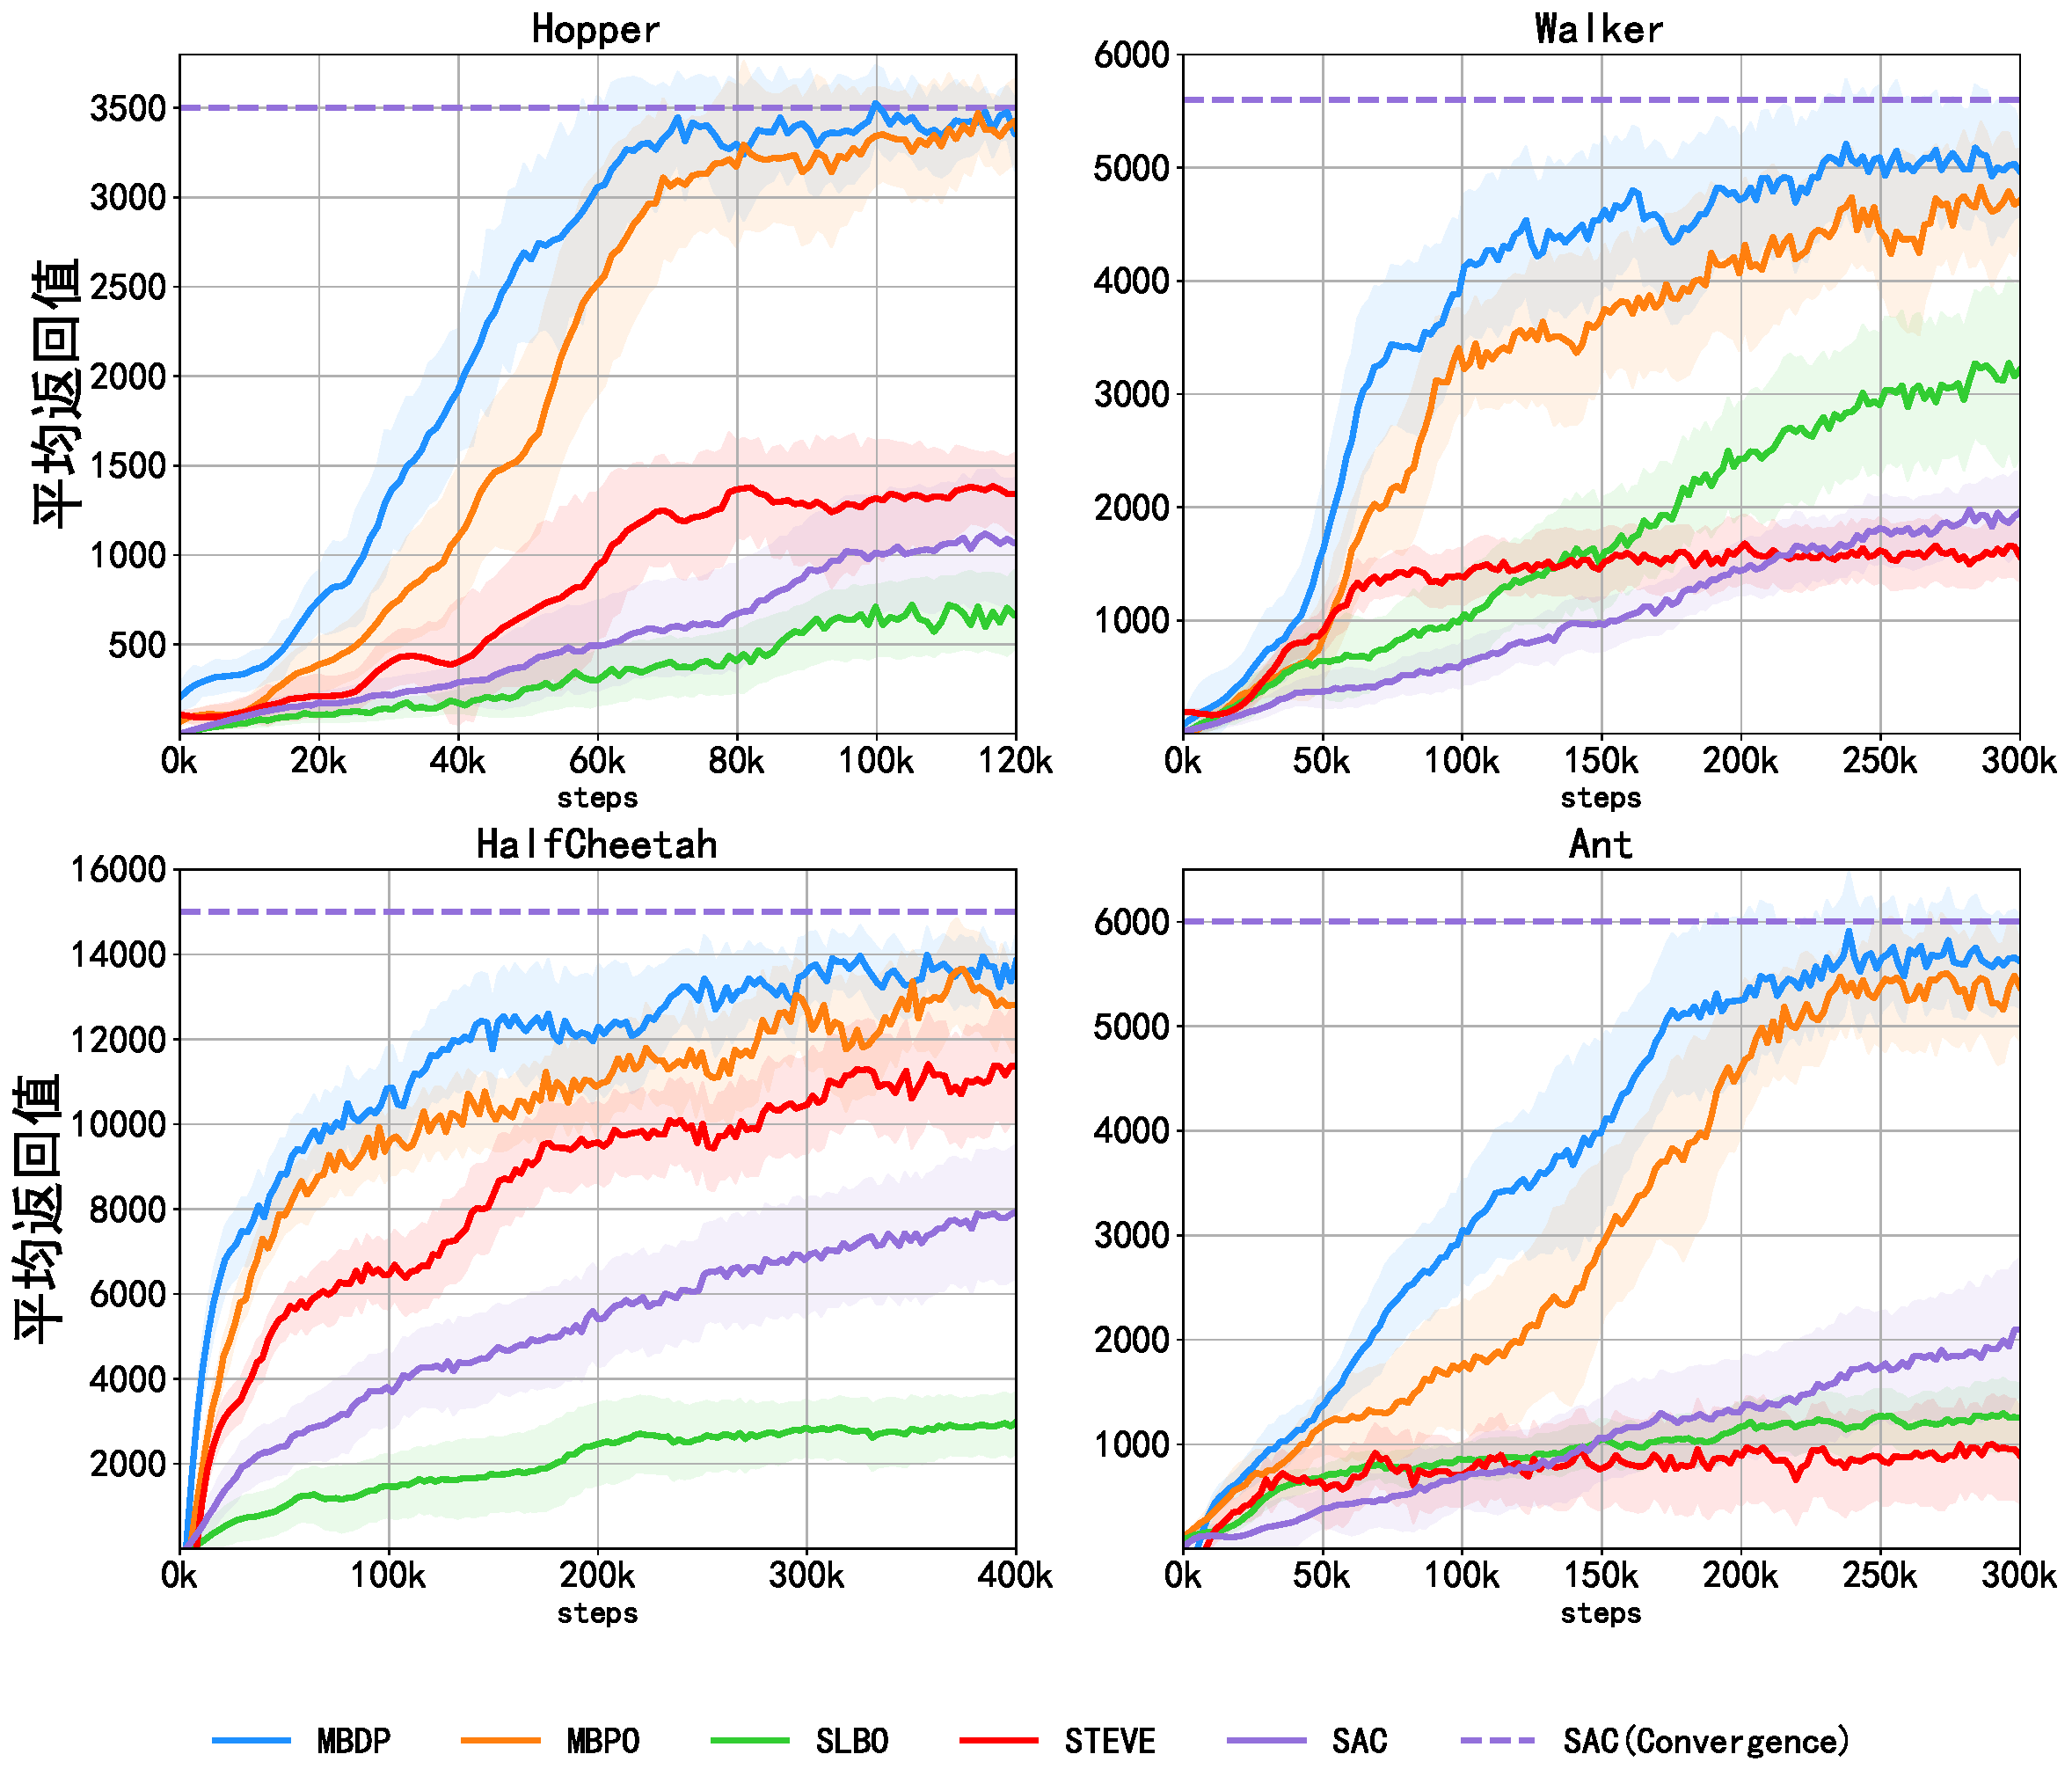
\includegraphics[width=\textwidth]{figures/performance.pdf}
  \caption{MBDP算法与基线算法在不同任务下的训练曲线图}
  \label{fig:performance}
\end{figure}

为了验证MBDP算法对鲁棒性的提升效果,本文对实验环境加入了不同程度的干扰。具体地,在Hopper和HalfCheetah两个任务环境下,将物体的质量和摩擦系数均加以数值区间为$[0.5,1.5]$的干扰,同时以MBPO算法作为对照标准进行对比实验。在每种干扰条件下均进行验证实验,Hopper任务中每组实验训练$3\times 10^5$轮,HalfCheetah任务中每组任务训练$6\times 10^5$轮,实验结果以热力图的形式绘制成图\ref{fig:robustness-heatmap},其中每一个方格表示一组干扰系数下训练相应轮数后的收益值。热力图中的颜色越接近红色代表该环境下的返回值越高,反之颜色越接近蓝色代表返回值越低。在该实验中,共设立了四种不同参数对应的算法,分别是$\alpha=0, \beta=0$的无筛选算法,$\alpha=0.2, \beta=0$的$\alpha$-筛选算法,$\alpha=0, \beta=0.2$的$\beta$-筛选算法以及$\alpha=0.2, \beta=0.2$的同时筛选算法。

显然可知,如果算法在整个热力图上的性能表现越一致,则说明该算法抗干扰能你更好,鲁棒性更高,反之若在热力图上的性能表现差异越大,则说明该算法更容易受环境干扰影响,鲁棒性更低。观察实验结果中的热力图,我们发现,仅使用模拟数据筛选模块的$\alpha$-筛选算法有着最好的鲁棒性提升,仅使用集成模型筛选模块的$\beta$-筛选算法则会带来鲁棒性下降的负面影响。而当将两种模块结合时,算法仍能维持较好的鲁棒性。这一实验验证了模拟数据筛选模块能够有效提升算法鲁棒性的结论,同时也证明了集成模型筛选模块和模拟数据筛选模块相结合后仍能有正向的鲁棒性提升效果。

\begin{figure}[t]
  \centering
  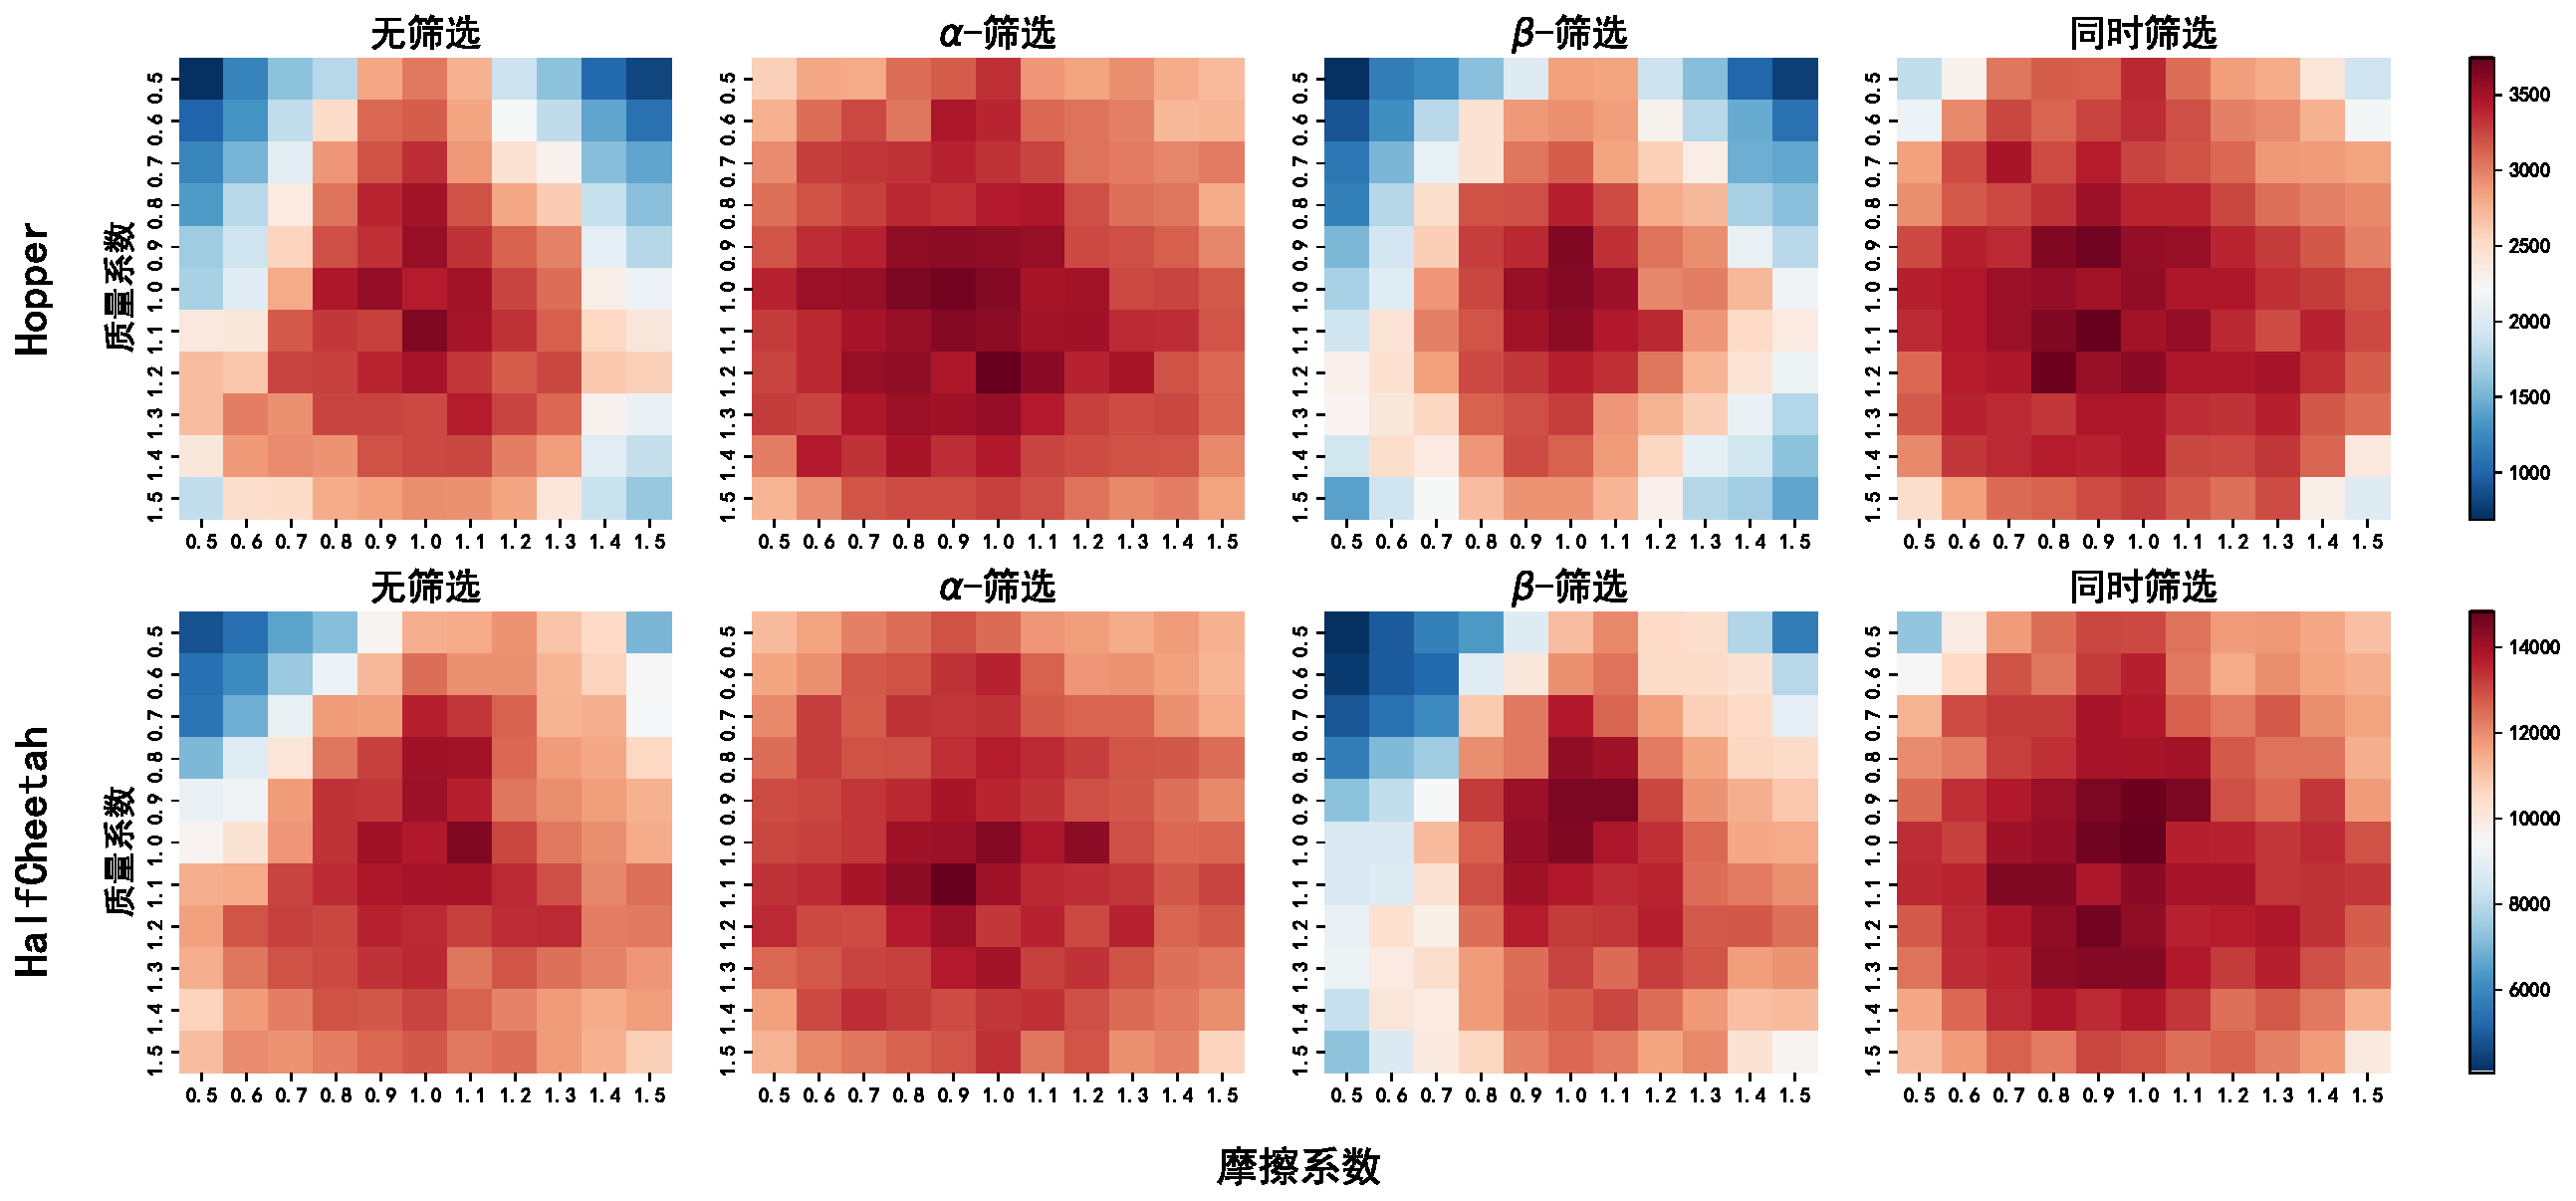
\includegraphics[width=\textwidth]{figures/robustness-heatmap.pdf}
  \caption{MBDP算法鲁棒性对比实验}
  \label{fig:robustness-heatmap}
\end{figure}

为了进一步验证参数$\alpha,\beta$和样本效率与鲁棒性的关系和敏感度,本文设计Hopper和HalfCheetah环境下的参数实验,实验分为两组:

\begin{enumerate}
    \item 固定参数$\beta=0.2$,将参数$\alpha$在区间$[0,0.5]$中由小到大进行调整
    \item 固定参数$\alpha=0.2$,将参数$\beta$在区间$[0,0.5]$中由小到大进行调整
\end{enumerate}

参数实验的结果如图~\ref{fig:hyper-performance}~所示。图中的第一行为Hopper环境下的实验结果,第二行为HalfCheetah环境下的实验结果。第1、2列为干扰环境实验组的实验结果,在干扰环境实验组中,我们针对每一组摩擦系数和质量系数构建了4种不同的干扰组合,具体地,将质量系数分别设为0.8和1.2,将摩擦系数分别设为0.8和1.2,总共组成$2\times 2=4$种干扰环境。在4个不同的干扰环境下分别进行策略学习,最终所能得到的平均返回值代表算法在受干扰环境中的综合评价指标,该指标越高,说明相应的参数$\alpha,\beta$能使得算法拥有更好的抗干扰性,也即鲁棒性。为了公平比较,我们在Hopper环境下统一训练120000步,在HalfCheetah环境下统一训练400000步。第3、4列为算法在标准环境(摩擦系数和质量系数均为1.0)下所能取得的返回值。同样的,我们在Hopper环境下统一训练120000步,在HalfCheetah环境下统一训练400000步。该项指标可用于评估不同参数下算法的样本利用效率。为了消除随机性的影响,每组实验均由10次随机种子实验组成,并将10次结果统计为箱线图。

观察实验结果,显然可以得出结论,样本利用效率与参数$\alpha$呈现负相关趋势,与参数$\beta$呈现正相关趋势;鲁棒性与参数$\alpha$呈现正相关趋势,与参数$\beta$呈现负相关趋势。这也验证了~\ref{sec:mbdp-description}~节中所提出的MBDP算法与样本利用效率和鲁棒性的关系。此外,我们在实验结果图中用水平虚线画出了不使用任何筛选模块的基线算法($\alpha=\beta=0$)性能,可以看出当$\alpha\in[0.1,0.2],\beta\in[0.1,0.2]$时,MBDP算法能同时得到样本利用效率和鲁棒性的提升。

\begin{figure}[t]
  \centering
  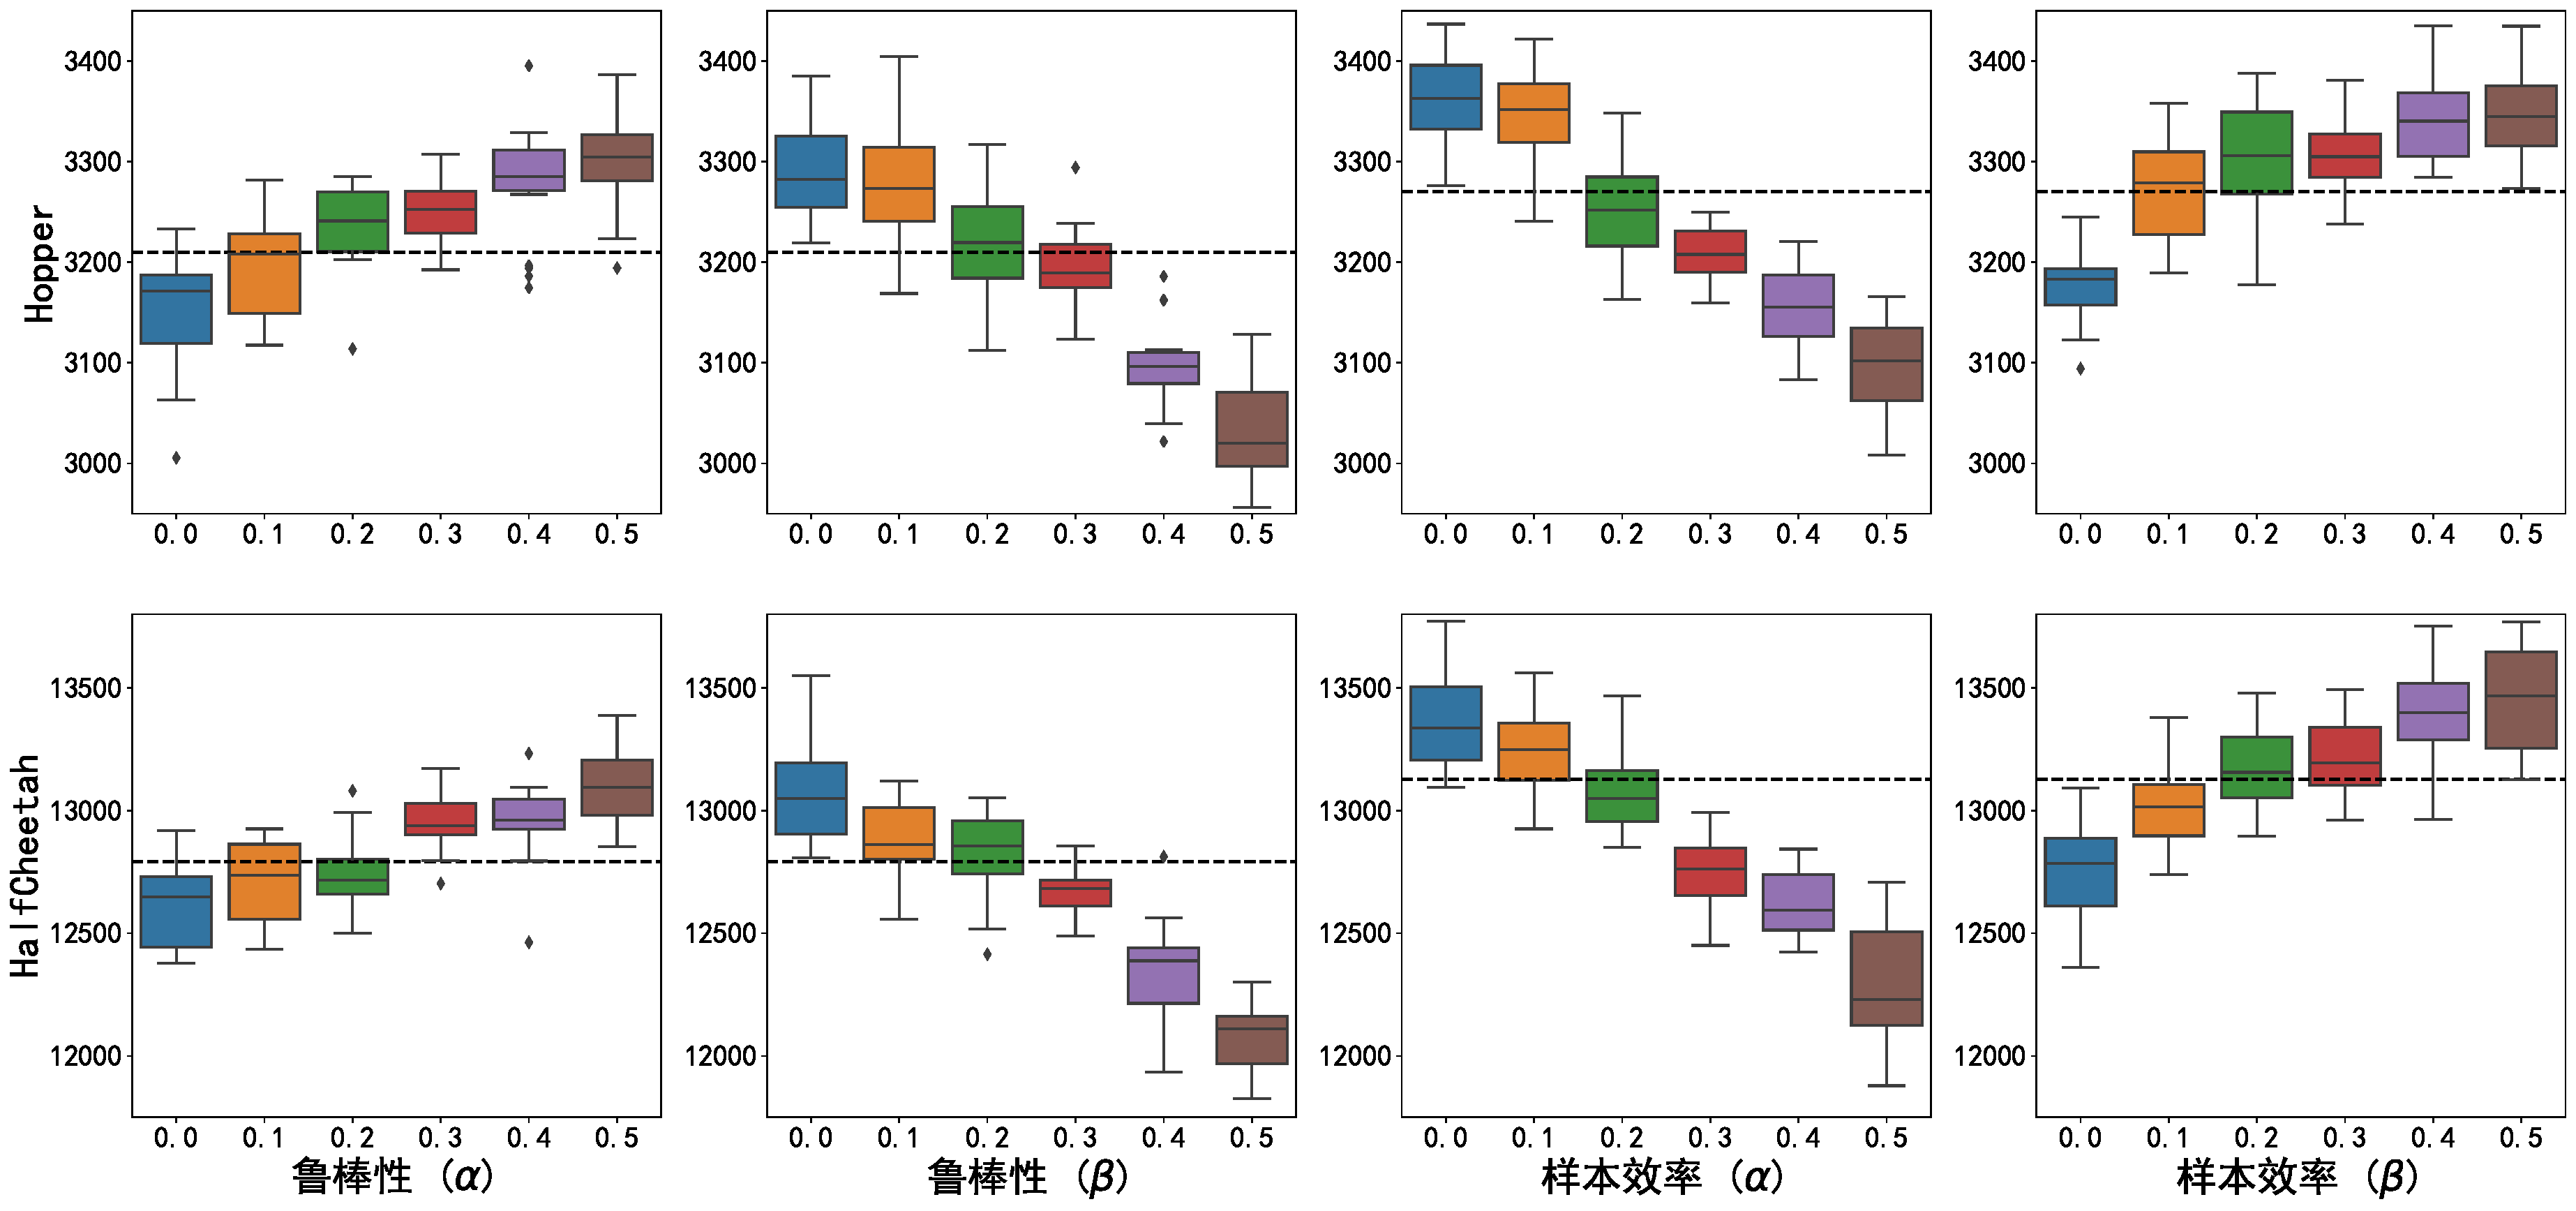
\includegraphics[width=\textwidth]{figures/hyper-performance.pdf}
  \caption{MBDP算法参数敏感性实验}
  \label{fig:hyper-performance}
\end{figure}

\section{本章小结}

本章主要介绍了针对强化学习的策略安全性问题提出的基于模型集成的筛选规划算法(Model-Based Dropout Planning,MBDP)。本工作提出了集成模型筛选模块和模拟数据筛选模块,它们共同组合构成了MBDP算法。其中集成模型筛选模块在模型集成方法的基础上,通过计算集成模型中单个模型的预测精确度,对所有模型进行排序,然后按精确度从大到小进行优先级筛选,以少量鲁棒性下降的代价换取模型集成整体精确性的提升,从而实现对算法整体起到样本利用效率的提升;而模拟数据模块则是在基于模型的强化学习方法的基础框架下,对状态转移模型所生成的模拟样本计算收益反馈值,然后排序并按收益值从小到大进行优先级筛选,以少量样本效率下降的代价换取对风险状态的关注程度,提升了策略的稳定性,从而对算法整体起到鲁棒性的提升。集成模型筛选模块和模拟数据筛选模块在对抗的作用下起到了兼顾样本效率提升和鲁棒性提升的平衡效果,其所学习得到的决策策略在保障样本效率的前提下,通过更优秀的鲁棒性来实现决策策略安全性的提升。在本章中,还通过详细的理论分析过程论证了集成模型筛选模块在样本利用效率上的提升效果和模拟数据筛选模块在鲁棒性上的提升效果。并进一步通过模拟仿真实验验证了上述结论。
% !TeX root = ../main.tex

\chapter{MBDP算法在决策控制任务中的应用}

\section{Mujoco控制任务}

在本课题中,为了证明上述改进方案的可行性,以及验证改进效果,本课题通过实验初步验证了2个问题:

\begin{itemize}
    \item 改进后的算法在强化学习的标准测试任务上相比最新的算法提升如何?
    \item 是否能达到\ref{sec:rollout-method}节中所描述的可以通过动态调整参数$\alpha,\beta$来取得不同决策策略的效果?
\end{itemize}

本课题使用强化学习中广泛使用的标准测试环境MuJoCo模拟器\cite{todorov2012mujoco}进行实验,首先在四组不同任务上,与最新的MBPO \cite{janner2019trust}算法、STEVE \cite{buckman2018sample}算法、SLBO \cite{Luo2019AlgorithmicGuarantees}算法以及无模型的SAC \cite{haarnoja2018soft}算法进行对比实验。在本课题的算法中,使用了参数$\alpha=0.5, \beta=0.85$。对比实验结果如图\ref{fig:performance}所示,其中横轴为训练的步数,纵轴为相应步数对应的平均收益。图中实线为不同随机种子实验的均值结果,阴影区域则表示这些实验的方差。由于SAC是无模型强化学习算法,相较基于模型的强化学习算法收敛速度较慢,因此只在图中画出部分训练曲线图,其最终收敛值通过虚线标注出来。

根据实验结果可以看出,本课题设计的改进算法在四种不同的任务环境中,均有着超越现有算法的表现。

\begin{figure}
  \centering
  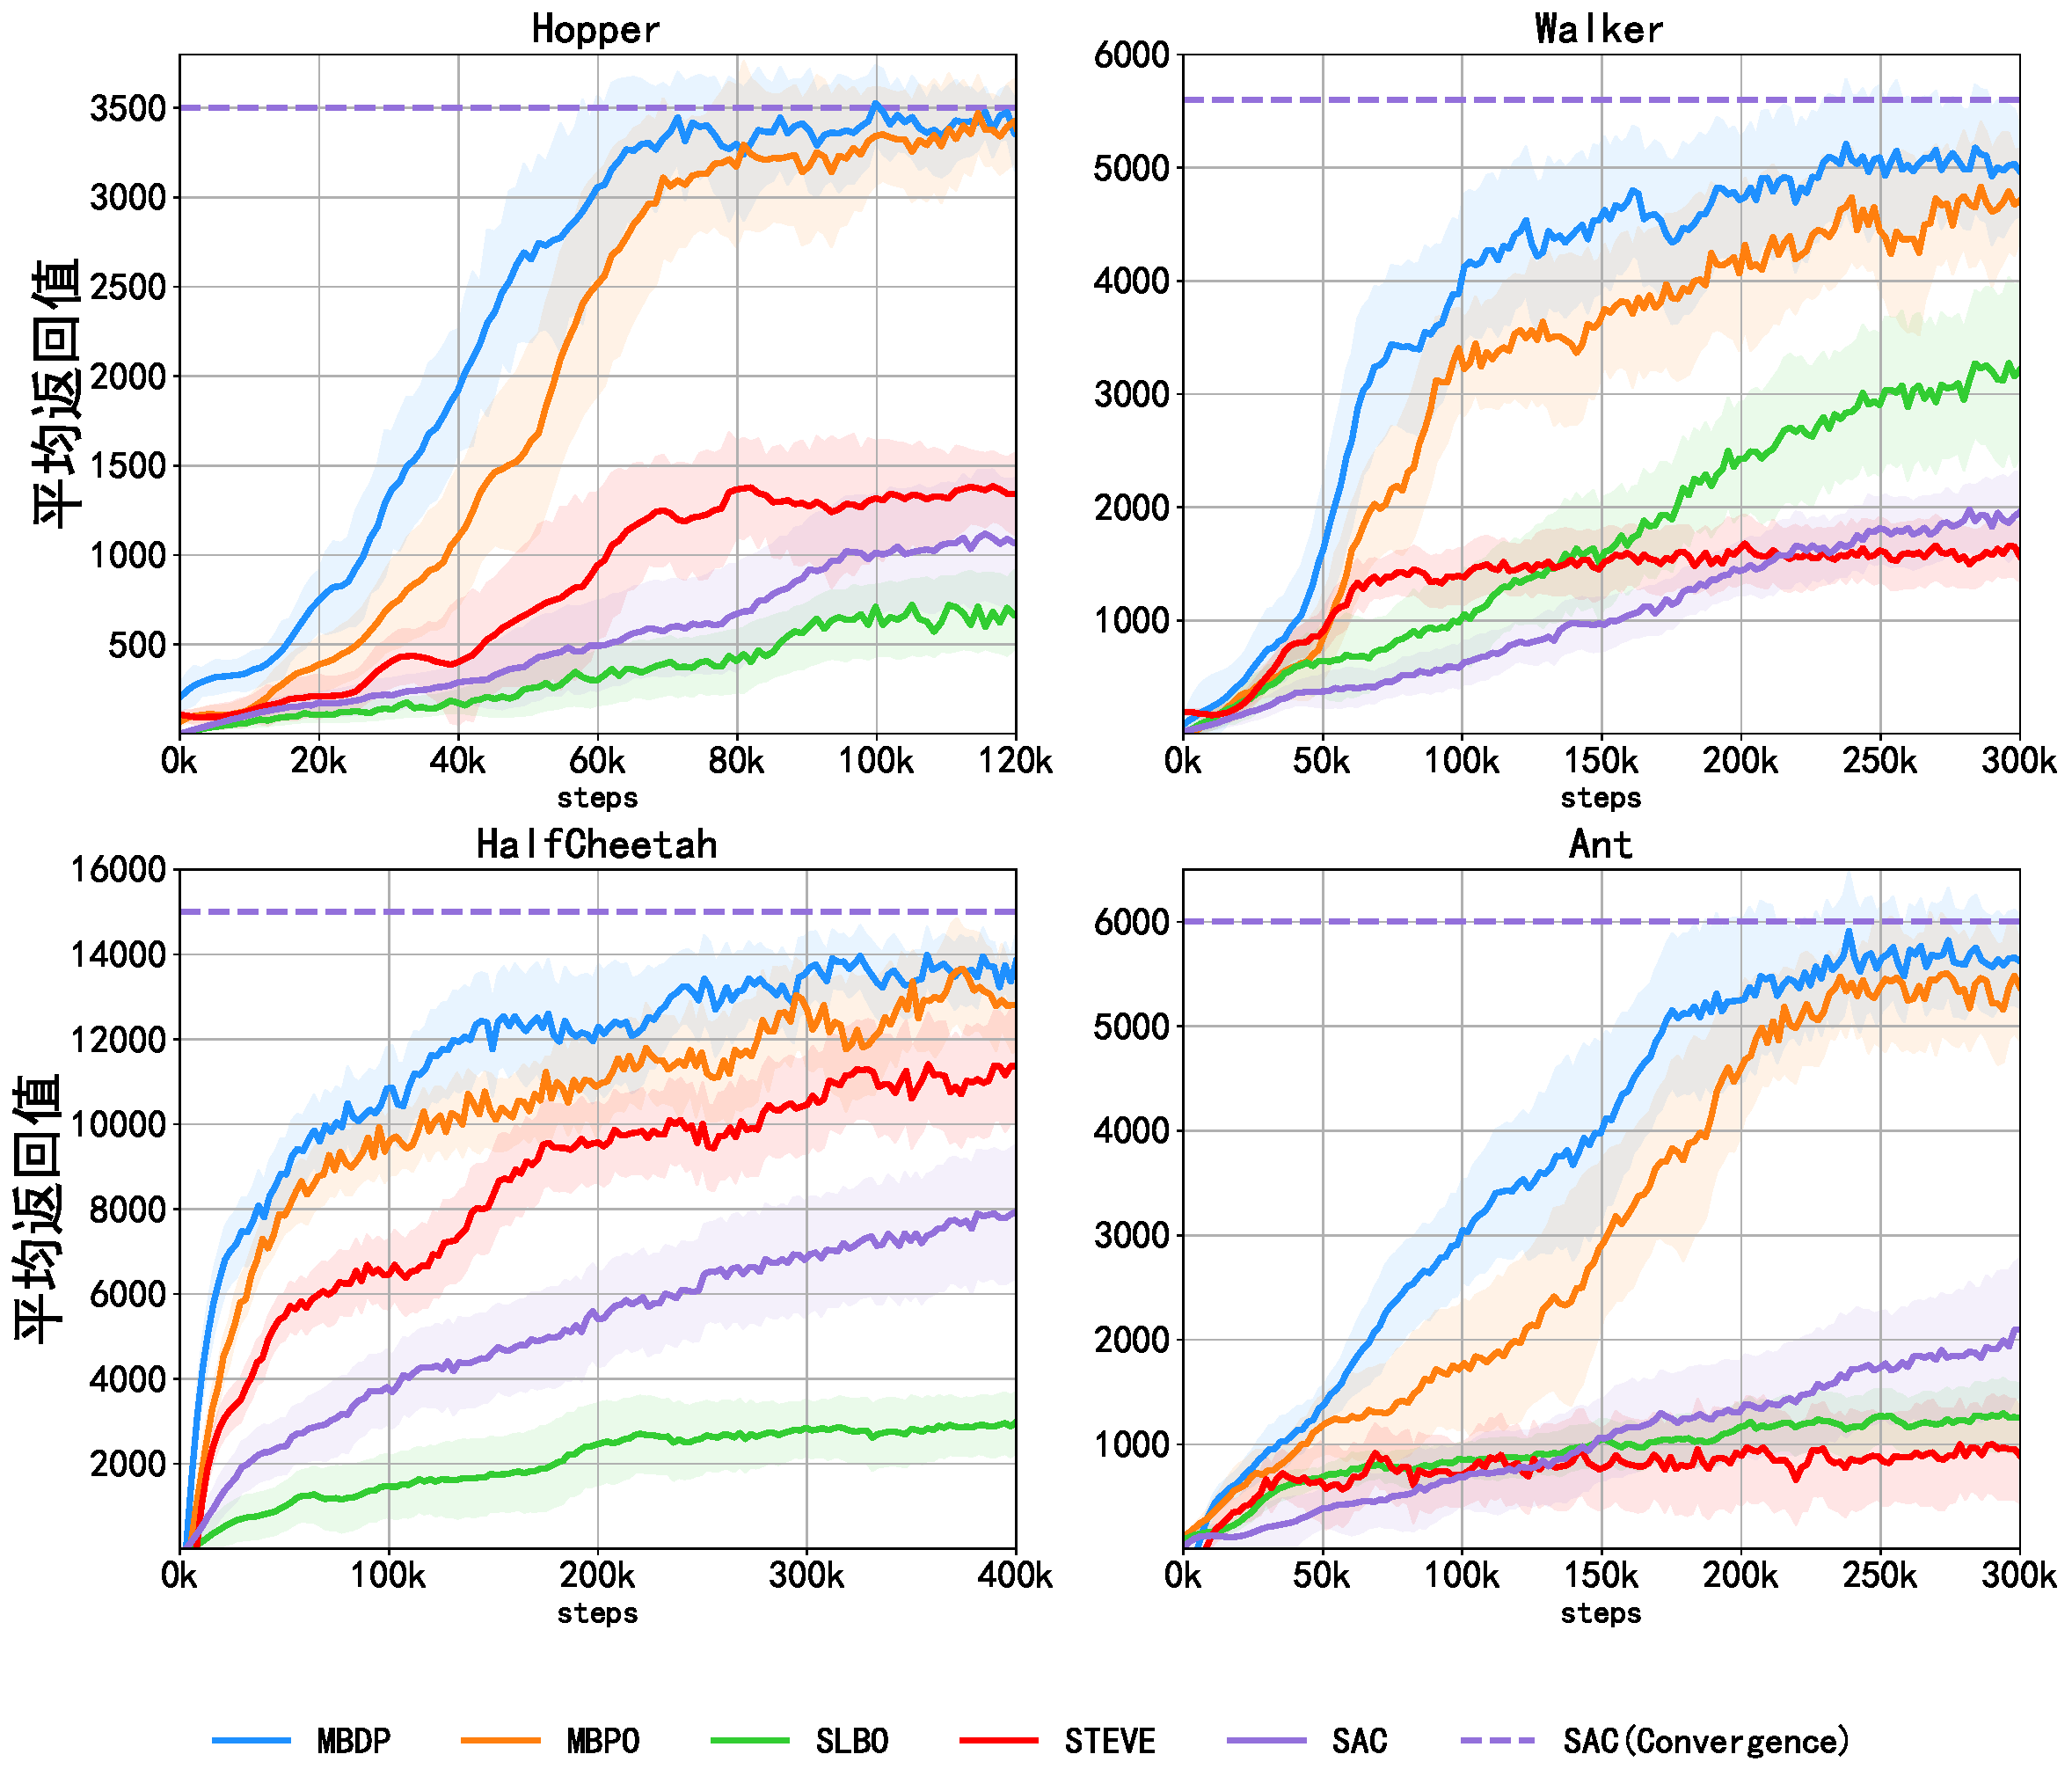
\includegraphics[width=0.9\textwidth]{figures/performance.pdf}
  \caption{各算法在不同任务下的训练曲线图。}
  \label{fig:performance}
\end{figure}

为了进一步验证改进算法的鲁棒性提升,对实验环境加入了不同程度的干扰,本课题在Hopper和HalfCheetah两个任务环境下,将物体的质量和摩擦系数均加以数值区间为$[0.5,1.5]$的干扰,同时以最新的MBPO算法作为对照标准进行对比实验。在各组干扰条件下均进行了一组实验,Hopper任务中每组实验训练$3\times 10^5$轮,HalfCheetah任务中每组任务训练$6\times 10^5$轮,实验结果以热力图的形式绘制成图\ref{fig:robustness-heatmap},其中每一个方格表示一组干扰系数下训练相应轮数后的收益值。观察实验结果可以看出,两种算法尽管在中间的正常区域有着接近的收益,但在干扰较大的环境中,作为对照的MBPO算法并不能有效地学习出决策策略,相比之下本课题的算法则能够较好地处理受干扰较大的环境,这一实验验证了本课题中设计的双筛选机制能够有效提升算法鲁棒性的结论。

\begin{figure}
  \centering
  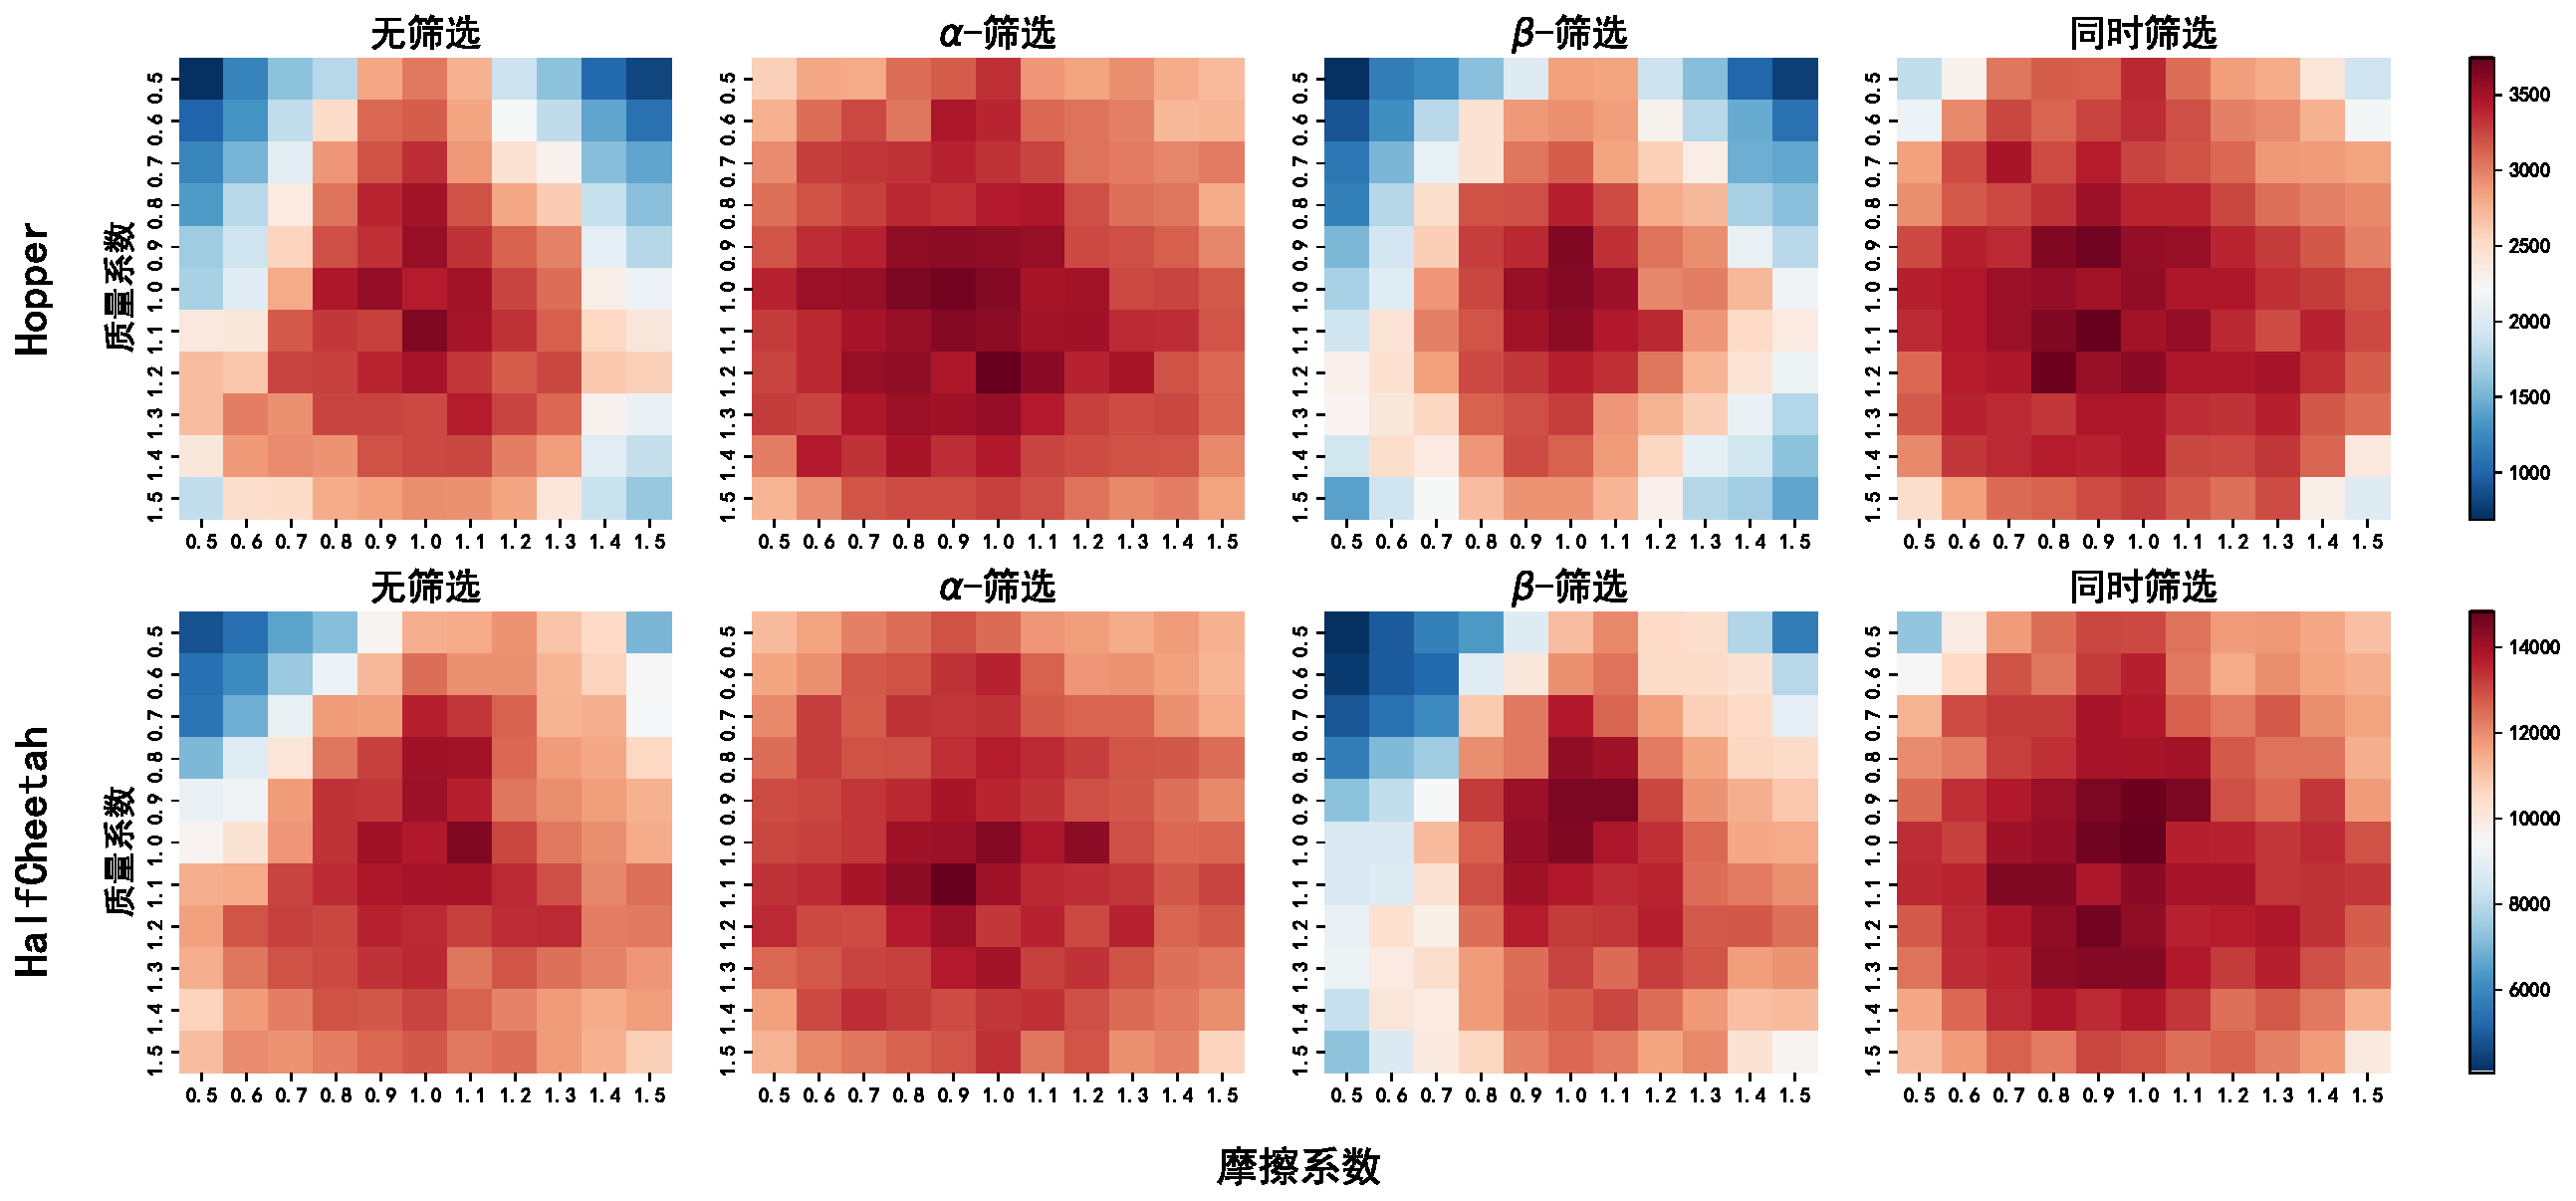
\includegraphics[width=0.7\textwidth]{figures/robustness-heatmap.pdf}
  \caption{算法鲁棒性对比实验。}
  \label{fig:robustness-heatmap}
\end{figure}

\section{自动化温室决策控制任务}

% !TeX root = ../main.tex

\chapter{总结与展望}\label{chap:summary}

\section{全文总结}

在智能决策学习任务中,算法的样本利用效率和所学策略的安全性往往限制了强化学习的实际应用效果,样本利用效率低下会带来高昂的采样成本,安全性的不足会导致策略做出不稳定甚至错误的决策。针对智能决策学习任务中的这些问题,本文首先提出基于双层缓存的优先经验回放算法(Double-layer Prioritized Experience Replay,DPER)和基于模型集成的筛选规划算法(Model-Based Dropout Planning,MBDP)。DPER算法通过在传统优先经验回放算法(PER)的基础上添加了第二层经验回放池,用于长时缓存全局空间的经验回放样本,达到进一步增加强化学习算法的样本利用效率的效果。而MBDP算法则以对抗的训练方式,设计了能够提升样本利用效率的集成模型筛选模块,以及能够提升算法鲁棒性的模拟数据筛选模块,两者结合而成的MBDP算法能够在保证算法样本利用效率的前提下,对鲁棒性起到大幅的提升作用。

本文首先在CliffWalking和OpenAI提供Mujoco环境下进行了模拟仿真实验,对所设计的DPER算法和MBDP算法进行了实验验证。实验表明,DPER算法中所提出的双层经验回放池设计能够有效地增强策略学习的收敛速度,相比优先经验算法(PER)有着更好的样本效率。而MBDP算法也在Mujoco环境下的验证实验中表现出了优秀的鲁棒性,即使环境发生干扰,也能一致地表现出收敛性能,验证了MBDP算法能够在保证算法样本利用率的同时,起到鲁棒性的提升效果这一结论。

为了进一步验证所提出的算法在真实应用场景中的提升效果,本文以基于模型集成的筛选规划算法为核心,针对自动化温室决策控制任务,设计了能够在温室中根据传感器信息自动控制设备的策略学习算法,并同时在仿真模拟器及真实环境中进行了验证实验。实验表明,算法不仅相比于普通的机器学习方法有着更好的收敛性能,还表现出了超越人类平均水平的决策性能。与此同时,算法在受环境干扰的情况下还表现出优异的稳定性,相比普通的机器学习算法,能够大幅提升自动化温室决策策略的安全性。这一实验结果也进一步地证明了本文所设计的算法能够在强化学习算法中有效提升样本利用效率和安全性。

\section{未来展望}

尽管强化学习算法在自动化决策控制任务中表现出强大的能力,但仍有大量的问题值得更加深入的探索。对于强化学习算法而言,智能体是在与环境反复循环交互的过程中通过不断试错并进行自我判断,对决策选项进行优化更新而最终收敛得到近似最优策略。然而在这一更新过程中,深度神经网络等黑箱模型的加入使得强化学习算法学习得到的策略产生了不可解释性,这也正是强化学习算法缺乏安全性的本质原因。尽管本文中提出的算法能够一定程度上缓解这一问题,但并没有在根源上得以解决。在未来的研究工作中,应该考虑更多开放式结构的白箱模型,使得模型学习和模型规划等环节能够得到可解释性的保障。

此外,本文所研究的样本利用效率问题和安全性问题均是基于单智能体的基本假设,而现实中的应用场景下,往往需要控制多智能体进行分工合作。相比于单智能体强化学习,多智能体背景下会面临更苛刻的样本利用效率问题和安全性问题,在本文的研究基础上,未来还需要将提出的DPER算法和MBDP算法拓展延伸至多智能体环境下,使得它们能够得到更广泛的应用。


% 其他部分
\backmatter

% 参考文献
\bibliography{ref/refs}  % 参考文献使用 BibTeX 编译
% \printbibliography       % 参考文献使用 BibLaTeX 编译

% 附录
\appendix
% % !TeX root = ../main.tex

\begin{survey}
\label{cha:survey}

\title{Title of the Survey}
\maketitle


\tableofcontents


本科生的外文资料调研阅读报告。


\section{Figures and Tables}

\subsection{Figures}

An example figure in appendix (Figure~\ref{fig:appendix-survey-figure}).

\begin{figure}
  \centering
  
\includegraphics[width=0.6\linewidth]{example-image-a.pdf}
  \caption{Example figure in appendix}
  \label{fig:appendix-survey-figure}
\end{figure}


\subsection{Tables}

An example table in appendix (Table~\ref{tab:appendix-survey-table}).

\begin{table}
  \centering
  \caption{Example table in appendix}
  \begin{tabular}{ll}
    \toprule
    File name       & Description                                         \\
    \midrule
    thuthesis.dtx   & The source file including documentaion and comments \\
    thuthesis.cls   & The template file                                   \\
    thuthesis-*.bst & BibTeX styles                                       \\
    thuthesis-*.bbx & BibLaTeX styles for bibliographies                  \\
    thuthesis-*.cbx & BibLaTeX styles for citations                       \\
    \bottomrule
  \end{tabular}
  \label{tab:appendix-survey-table}
\end{table}


\section{Equations}

An example equation in appendix (Equation~\eqref{eq:appendix-survey-equation}).
\begin{equation}
  \frac{1}{2 \uppi \symup{i}} \int_\gamma f = \sum_{k=1}^m n(\gamma; a_k) \mathscr{R}(f; a_k)
  \label{eq:appendix-survey-equation}
\end{equation}


\section{Citations}

Example citations in appendix.
\cite{abrahams99tex}
\cite{salomon1995advanced}
\cite{abrahams99tex,salomon1995advanced}


\bibliographystyle{unsrtnat}
\bibliography{ref/appendix}

\end{survey}
       % 本科生:外文资料的调研阅读报告
% % !TeX root = ../main.tex

\begin{translation}
\label{cha:translation}

\title{书面翻译题目}
\maketitle

\tableofcontents


本科生的外文资料书面翻译。


\section{图表示例}

\subsection{图}

附录中的图片示例(图~\ref{fig:appendix-translation-figure})。

\begin{figure}
  \centering
  
\includegraphics[width=0.6\linewidth]{example-image-a.pdf}
  \caption{附录中的图片示例}
  \label{fig:appendix-translation-figure}
\end{figure}


\subsection{表格}

附录中的表格示例(表~\ref{tab:appendix-translation-table})。

\begin{table}
  \centering
  \caption{附录中的表格示例}
  \begin{tabular}{ll}
    \toprule
    文件名          & 描述                         \\
    \midrule
    thuthesis.dtx   & 模板的源文件,包括文档和注释 \\
    thuthesis.cls   & 模板文件                     \\
    thuthesis-*.bst & BibTeX 参考文献表样式文件    \\
    thuthesis-*.bbx & BibLaTeX 参考文献表样式文件  \\
    thuthesis-*.cbx & BibLaTeX 引用样式文件        \\
    \bottomrule
  \end{tabular}
  \label{tab:appendix-translation-table}
\end{table}


\section{数学公式}

附录中的数学公式示例(公式\eqref{eq:appendix-translation-equation})。
\begin{equation}
  \frac{1}{2 \uppi \symup{i}} \int_\gamma f = \sum_{k=1}^m n(\gamma; a_k) \mathscr{R}(f; a_k)
  \label{eq:appendix-translation-equation}
\end{equation}


\section{文献引用}

文献引用示例\cite{abrahams99tex}。


% 书面翻译的参考文献
\bibliographystyle{unsrtnat}
\bibliography{ref/appendix}

% 书面翻译对应的原文索引
\begin{translation-index}
  \nocite{salomon1995advanced}
  \bibliographystyle{unsrtnat}
  \bibliography{ref/appendix}
\end{translation-index}

\end{translation}
  % 本科生:外文资料的书面翻译
% !TeX root = ../main.tex

\chapter{补充内容}

附录


\section{图表示例}

图。

% 致谢
% !TeX root = ../main.tex

\begin{acknowledgements}
在清华的三年研究生时光已接近尾声,这三年收获颇多,受益匪浅,衷心感谢我的导师肖喜副教授、计算机系夏树涛教授、北京大学的卢宗青老师和腾讯AI Lab的罗迪君博士对本人的帮助和精心指导,他们的言传身教将使我终生收益。无论是学业上的精进和方法上的指点,抑或科研上的启发和思想上的碰撞,均有他们的身影引领我迈上学术的道路,让我在浩瀚无垠的学海中找到方向。

同时,我也要感谢父母和家人对我无微不至的关照和坚定的信任支持,没有他们在我身后的无私付出,就没有我成长至今的一切成就。

其次,我要感谢在我生活中陪伴我一路走来的同窗和朋友。感谢陈明哲、陈煜钊、魏子瑜、张焓祺,与你们一起思考、一同进步是我莫大的荣幸。感谢室友金涛、宋星辰,你们的包容和陪伴让我的三年时光添满色彩。特别感谢张绰棋和张雪曼,作为心灵上的支撑,你们的陪伴和宽慰是我不断前进的动力!

最后,我要感谢所有帮助过我的人,谢谢你们的关心、支持、和肯定,我会继续努力,带着你们的信任,迈向人生新的高度。
\end{acknowledgements}


% 声明
\statement
% 将签字扫描后的声明文件 scan-statement.pdf 替换原始页面
% \statement[file=scan-statement.pdf]
% 本科生编译生成的声明页默认不加页脚,插入扫描版时再补上;
% 研究生编译生成时有页眉页脚,插入扫描版时不再重复。
% 也可以手动控制是否加页眉页脚
% \statement[page-style=empty]
% \statement[file=scan-statement.pdf, page-style=plain]

% 个人简历、在学期间完成的相关学术成果
% !TeX root = ../main.tex

\begin{resume}

  \section*{个人简历}

  1997 年 11 月 30 日出生于四川省成都市。

  2015 年 9 月考入南开大学数学系信息与计算科学专业,2019 年 7 月本科毕业并获得理学学士学位。

  2019 年 9 月免试进入清华大学计算机科学与技术系攻读计算机技术专业硕士研究生至今。


  \section*{在学期间完成的相关学术成果}

  \subsection*{已发表学术论文}

  \begin{achievements}
    \item \textbf{Wanpeng Zhang}, Xiaoyan Cao, Yao Yao, Zhicheng An, Dijun Luo, Xi Xiao. Robust Model-based Reinforcement Learning for Autonomous Greenhouse Control[C]//Asian Conference on Machine Learning. PMLR, 2021: 1208-1223.
    \item Bowen Zhao, Xi Xiao, \textbf{Wanpeng Zhang}, Bin Zhang, Guojun Gan, Shutao Xia. Self-paced probabilistic principal component analysis for data with outliers[C]//ICASSP 2020-2020 IEEE International Conference on Acoustics, Speech and Signal Processing (ICASSP). IEEE, 2020: 3737-3741.
    \item Mingzhe Chen, Xi Xiao, \textbf{Wanpeng Zhang}, Xiaotian Gao. Efficient And Stable Information Directed Exploration For Continuous Reinforcement Learning[C]//ICASSP 2022-2022 IEEE International Conference on Acoustics, Speech and Signal Processing (ICASSP). IEEE, 2022: 4023-4027.
    \item Yao Yao, Li Xiao, Zhicheng An, \textbf{Wanpeng Zhang}, Dijun Luo. Sample Efficient Reinforcement Learning via Model-Ensemble Exploration and Exploitation[C]//2021 IEEE International Conference on Robotics and Automation (ICRA). IEEE, 2021: 4202-4208.
    \item Zhicheng An, Xiaoyan Cao, Yao Yao, \textbf{Wanpeng Zhang}, Lanqing Li, Yue Wang, Shihui Guo, Dijun Luo. A Simulator-based Planning Framework for Optimizing Autonomous Greenhouse Control Strategy[C]//Proceedings of the International Conference on Automated Planning and Scheduling. 2021, 31: 436-444.
    \item Zhicheng An, Xiaoyan Cao, Yao Yao, \textbf{Wanpeng Zhang}, Lanqing Li, Yue Wang, Shihui Guo, Dijun Luo. iGrow: A Smart Agriculture Solution to Autonomous Greenhouse Control[C].//Proceedings of the AAAI Conference on Artificial Intelligence. 2022.
  \end{achievements}
  
  \subsection*{在投学术论文}
  \begin{achievements}
    \item \textbf{Wanpeng Zhang}, Xi Xiao, Yao Yao, Mingzhe Chen, Dijun Luo. MBDP: A Model-based Approach to Achieve both Robustness and Sample Efficiency via Double Dropout Planning. Submitted to Artificial Intelligence.
    \item \textbf{Wanpeng Zhang}, Xi Xiao, Bin Zhang, Guojun Gan. DPER: Double Layer Prioritized Experience Replay for Enhancing Model Based Reinforcement Learning. Submitted to IROS 2022.
    \item Xiaopeng Yu, Jiechuan Jiang, \textbf{Wanpeng Zhang}, Haobin Jiang, Zongqing Lu. Model-Based Opponent Modeling. Submitted to NeurIPS 2022.
  \end{achievements}


  \subsection*{专利}

  \begin{achievements}
    \item 张万鹏,罗迪君,肖喜. 确定参数确定方法、装置、设备及存储介质. 专利申请号:CN202011331054.8(已公开)
  \end{achievements}
  
    \section*{参与的科研项目}
    \begin{enumerate}[{[}1{]\;\;\;}]
        \item 国家自然科学基金面上项目:流量数据驱动的鲁棒自适应分类算法研究(61972219)
        \item 国家重点研发计划项目:自主可控高性能路由器及关键技术(2018YFB1800601)
        \item 深圳市基础研究面上项目:网络谣言检测及危害评估研究(JCYJ20190813174403598)
        \item 深港联合资助项目:基于区块链及操作的数据保护技术研发与应用(SGDX20190918101201696)
    \end{enumerate}

\end{resume}


% 指导教师/指导小组学术评语
% !TeX root = ../main.tex

\begin{comments}
% \begin{comments}[name = {指导小组学术评语}]
% \begin{comments}[name = {Comments from Thesis Supervisor}]
% \begin{comments}[name = {Comments from Thesis Supervision Committee}]

强化学习算法是一种高效的智能决策方法。但样本利用效率和策略安全性是其应用于真实场景的关键瓶颈之一。优先经验回放算法通过改变回放样本分布,优先学习部分样本的做法提升了样本利用效率。基于模型的强化学习算法通过对环境建模产生模拟数据辅助学习,也能加快学习速度。两者均是解决样本利用效率的较好思路,但这些方法在提升样本利用效率的同时,无法保证策略的稳定性。

该论文针对以上问题,开展了对强化学习算法的样本利用效率和安全性研究,选题具有重要价值。论文主要取得了以下几个成果: 

\begin{enumerate}
    \item 提出了一种基于双层缓存的优先经验回放算法(Double-layer Prioritized Experience Replay,DPER),通过双层经验回放池的设计,以不同速率进行优先级经验回放,在同等的样本消耗量下,实现了对样本空间更大的经验回放覆盖率,有效提升了强化学习算法的样本利用效率。
    \item 提出了一种基于模型集成的筛选规划算法(Model-Based Dropout Planning,MBDP),通过将集成模型筛选模块和模拟数据筛选模块相整合,以对抗的学习方式,设计了一个可以动态取舍样本利用效率和策略鲁棒性的算法框架,最终实现了在保证样本利用效率的前提下对所学决策策略安全性进行有效的加强。
    \item 在真实温室环境中,将所提出的DPER算法与MBDP算法整合,设计了自动化控制策略学习框架,在严苛的条件下对提出的算法进行了全面充分的验证,对于强化学习算法在真实复杂场景中的可应用性有重要意义。
\end{enumerate}

 论文结构合理,层次清晰,文献详实,实验充分,用词准确,将自己的工作进行了详细的阐述。论文工作表明该同学已掌握本学科坚实的理论基础知识,具有较强学习能力和动手能力,具备独立从事科学研究的能力。论文达到了工学硕士学位论文的要求,同意其答辩申请,并建议安排答辩。

\end{comments}


% 答辩委员会决议书
% !TeX root = ../main.tex

\begin{resolution}

  论文提出了……

  论文取得的主要创新性成果包括:

  1. ……

  2. ……

  3. ……

  论文工作表明作者在×××××具有×××××知识,具有××××能力,论文××××,答辩××××。

  答辩委员会表决,(×票/一致)同意通过论文答辩,并建议授予×××(姓名)×××(门类)学博士/硕士学位。

\end{resolution}


% 本科生的综合论文训练记录表(扫描版)
% \record{file=scan-record.pdf}

\end{document}
